% ------------------------------------------------------------
% $Id: repository.tex 6260 2010-08-15 02:36:26Z al $
% ------------------------------------------------------------
\documentclass[12pt]{book}
\usepackage{fancyhdr}
\renewcommand{\chaptermark}[1]{\markboth{#1}{}}
\fancyhf{} % delete current setting for header and footer
\fancyhead[RO,LE]{\bfseries\thepage}
\fancyhead[LO]{\bfseries\leftmark}
\fancyhead[RE]{\bfseries\leftmark}
\renewcommand{\headrulewidth}{0.5pt}
\renewcommand{\footrulewidth}{0pt}
\addtolength{\headheight}{0.5pt} % make space for the rule
\fancypagestyle{plain}{%
   \fancyhead{} % get rid of headers on plain pages
   \renewcommand{\headrulewidth}{0pt} % and the line
   }
\usepackage[pdftex]{graphicx}
\usepackage{hyperref}
\hypersetup{pdfauthor={Alain Reguera Delgado},%
            pdftitle={The CentOS Project - Artwork Repository},%
            pdfsubject={CentOS Corporate Visual Identity}%
            }

\title{The CentOS Project - Artwork Repository}
\author{Alain Reguera Delgado}

% Define words you don't want to split.
\hyphenation{CentOS}

\begin{document}

\pagestyle{empty}

% Half title: The first page is a recto half title page with no folio.
% The page is very simple and displays just the main title of the book
% — no subtitle, author, or other information. One purported purpose
% of this page is to protect the main title page.
\begin{titlepage}
\begin{flushright}
\noindent
\includegraphics[width=1\textwidth]{%
    /home/centos/artwork/trunk/Identity/Models/Img/en/Promo/Stationery/motif-propagation.pdf}\\
\vspace*{150pt}
\Huge\textbf{The CentOS Project}
\rule{\textwidth}{5pt}
\large
\textbf{Artwork Repository}\\
\vspace*{150pt}
\normalsize
\today
\end{flushright}
\end{titlepage}

% Page title: The title page is recto and contains the full title of
% the work, the names of the author(s) or editor(s), and often at the
% bottom of the page the name of the publisher, together with the
% publisher’s logo if it has one.
\begin{titlepage}
\begin{flushright}
\noindent
\includegraphics[width=1\textwidth]{%
    /home/centos/artwork/trunk/Identity/Models/Img/en/Promo/Stationery/motif-propagation.pdf}\\
\vspace*{150pt}
\Huge\textbf{The CentOS Project}
\rule{\textwidth}{5pt}
\large
\textbf{Artwork Repository}\\
\vspace*{150pt}
\normalsize
Alain Reguera Delgado $<$alain.reguera@gmail.com$>$\\
\end{flushright}
\end{titlepage}

% Copyright: The copyright page is verso and contains the copyright
% notice, the publishing/printing history, the country where printed,
% ISBN and/or CIP information.  The page is usually typeset in a
% smaller font than the normal text.

\noindent Copyright \copyright\ 2009, 2010 Alain Reguera Delgado. All\
rights reserved.\\
\\
\noindent Permission is granted to copy, distribute and/or modify this
document under the terms of the GNU Free Documentation License,
Version 1.2 or any later version published by the Free Software
Foundation; with no Invariant Sections, no Front-Cover Texts, and no
Back-Cover Texts. A copy of the license is included in the section
entitled ``\hyperlink{cha:Licenses:GFDL}{GNU Free Documentation
License}''.  

\frontmatter
\pagestyle{fancy}

% Listings:
\tableofcontents
\listoftables
\listoffigures

% Reset fancyhdr marks.
\renewcommand{\chaptermark}[1]{\markboth{#1}{}}

% Dedication:
%\chapter*{Dedication}

% Forewords: There may be a foreword after the listings, with no blank
% separator. A foreword is usually written by someone other than the
% author, preferably an eminent person, and is signed by the writer.
% The writer’s signature is often typeset in small caps after the end
% of the piece.
%\chapter{Forewords}

% Preface: A preface is normally written by the author, in which he
% includes reasons why he wrote the work in the first place, and
% perhaps to provide some more personal comments than would be
% justified in the body. A preface starts on the page immediately
% following a foreword, or the lists.
%\chapter{Preface}

\mainmatter

% Reset fancyhdr marks.
\renewcommand{\chaptermark}[1]{\markboth{%
   \chaptername\ \thechapter.\ #1}{}}

\part{Concepts}

\chapter{The CentOS Project}
   \hypertarget{cha:Concepts:CentOS}{}
   \label{cha:Concepts:CentOS}
   %    Part: Distribution
% Chapter: Anaconda Progress - Introduction
% ------------------------------------------------------------
% $Id: introduction.tex 6019 2010-06-26 06:42:08Z al $
% ------------------------------------------------------------

Anaconda progress takes place after configuration screens and while
packages are being installed.  Anaconda progress visual style is
controlled by ``\hyperlink{cha:Distribution:Anaconda:Header}{Anaconda
Header}'' (\autoref{cha:Distribution:Anaconda:Header}), Anaconda
progress first slide, and Anaconda progress language-specific slides
set of images. Anaconda progress language-specific slides set of
images start rotating a few seconds after Anaconda progress first
slide.  It is possible for the user to alternate between Anaconda
progress slides and CentOS distribution
``\hyperlink{cha:Distribution:ReleaseNotes}{Release Notes}''
(\autoref{cha:Distribution:ReleaseNotes}).


   
\section{The CentOS Incorporation}

The CentOS Project is a legal entity separate from the persons who own
it or the persons who manage or operate it.


   
\section{The CentOS Philosophy}

The CentOS Project is higly based on meritocracy.


   % ------------------------------------------------------------
% $Id: mission.tex 6024 2010-06-28 04:28:27Z al $
% ------------------------------------------------------------
    \section{The CentOS Mission}
\hypertarget{sec:Concepts:CentOS:Mission}{}
      \label{sec:Concepts:CentOS:Mission}

The CentOS Project exists to provide the CentOS Distribution. 


   % ------------------------------------------------------------
% $Id: distribution.tex 6024 2010-06-28 04:28:27Z al $
% ------------------------------------------------------------
    \section{The CentOS Distribution}
\hypertarget{sec:Concepts:CentOS:Distribution}{}
      \label{sec:Concepts:CentOS:Distribution}

The CentOS Distribution is a free enterprise class computing platform
to anyone who wishes to use it.  The CentOS Distribution is built from
publicly available open source SRPMS provided by a prominent North
American Enterprise Linux vendor.  The CentOS Distribution conforms
fully with the upstream vendors redistribution policies and aims to be
100\% binary compatible (The CentOS Project mainly changes packages to
remove upstream vendor branding and artwork.).

The CentOS Project releases its CentOS Distribution as a GPL work. The
GPL applies to the software collection known as the CentOS
Distribution.  Individual packages included in the distribution
include their own licenses and the GPL applies to all packages that it
does not clash with. If there is a clash between the GPL and
individual package licenses, the individual package license applies
instead.

Neither the CentOS Project (we who build CentOS Distribution) nor any
version of CentOS Distribution is affiliated with, produced by, or
supported by the prominent North American Enterprise Linux vendor.
Neither does our software contain the upstream vendor's product \dots
although it is built from the same open source SRPMS as the upstream
enterprise products.


   % ------------------------------------------------------------
% $Id: community.tex 6024 2010-06-28 04:28:27Z al $
% ------------------------------------------------------------
    \section{The CentOS Community}
\hypertarget{sec:Concepts:CentOS:Community}{}
      \label{sec:Concepts:CentOS:Community}

The CentOS Project is designed for people who need an enterprise class
operating system without the cost or support of the prominent North
American Enterprise Linux vendor.

\begin{description}

\item[CentOS Administrators:] People building CentOS Distribution and
its infrastructure are considered CentOS Administrators. Each CentOS
Distribution has an Administrator Leader.

\item[CentOS Community Members:] People using CentOS Distribution are
concidered CentOS Community Members.  Inside CentOS Community, Members
affiliate Special Interest Groups (SIGs). Special Interest Groups help
to organize and distribute work inside The CentOS Project.

\end{description}

   % Part   : Concepts
% Chapter: Corporate Identity
% ------------------------------------------------------------
% $Id: release.tex 6023 2010-06-27 10:09:48Z al $
% ------------------------------------------------------------

\section{Release}
\hypertarget{sec:Concepts:Identity:Release}{}
\label{sec:Concepts:Identity:Release}

\begin{description}
\item[framework:] trunk/Identity/Release/
\end{description}

\noindent Here is where CentOS Distribution release-specific files are
produced.  This framework contains textual templates that produce
textual files, like ``release notes'' and ``eula files'' used by
Anaconda.



\chapter{Frameworks}
   \hypertarget{cha:Concepts:frameworks}{}
   \label{cha:Concepts:Frameworks}
   %    Part: Distribution
% Chapter: Anaconda Progress - Introduction
% ------------------------------------------------------------
% $Id: introduction.tex 6019 2010-06-26 06:42:08Z al $
% ------------------------------------------------------------

Anaconda progress takes place after configuration screens and while
packages are being installed.  Anaconda progress visual style is
controlled by ``\hyperlink{cha:Distribution:Anaconda:Header}{Anaconda
Header}'' (\autoref{cha:Distribution:Anaconda:Header}), Anaconda
progress first slide, and Anaconda progress language-specific slides
set of images. Anaconda progress language-specific slides set of
images start rotating a few seconds after Anaconda progress first
slide.  It is possible for the user to alternate between Anaconda
progress slides and CentOS distribution
``\hyperlink{cha:Distribution:ReleaseNotes}{Release Notes}''
(\autoref{cha:Distribution:ReleaseNotes}).


   % Part   : Concepts
% Chapter: Frameworks
% ------------------------------------------------------------
% $Id: templates.tex 6207 2010-08-05 13:11:13Z al $
% ------------------------------------------------------------

\section{Design Templates}
\hypertarget{sec:Concepts:Frameworks:Templates}{}
\label{sec:Concepts:Frameworks:Templates}

Design templates are plain text files. Design templates may or may not
contain translation markers inside.  Design templates are used to
define the CentOS visual style (the look and feel) of CentOS corporate
identity in all its manifestations.  Design templates are the
documents you need to create or edit in order to implement or maintain
the monolithic CentOS corporate visual structure.  Design templates
are normative documents that need to be conceived carefully.

Design templates may be based on specific markups (i.e. XHTML, SVG,
CSS, etc.). If that is the case, translation markers may be combined
inside the specific markup design template to create a translatable
markup-specific design template. In contrast, if design templates do
not have specific markup inside, they are considered the simpliest
design templates because they only have translation markers inside.

Design templates can be read, edited, and studied using your favorite
text editor. 

Design templates are specific to frameworks using design patterns to
define the visual style of content produced inside them.  This is the
case of frameworks inside ``trunk/Identity/'', where design templates
are used to define images' visual style; and ``trunk/Translations/'',
where design tempates are used to define translations' common files.

Inside frameworks, design templates are stored in a directory named
`tpl'. This name is a convenction that scripts use to find framework's
design tempate files. If you want to change the design template
directory's name to something different from `tpl', you need to set
the same name in all design templates' directories along the CentOS
Artwork Repository, and update scripts to recognize the new name you
set.  This is something you problably don't need to do, but if you
still want to, please share your reasons in
\href{mailto:centos-devel@centos.org}{centos-devel@centos.org} before
commit your changes. Changing the design template directory's name is
a big chanage that needs to be discussed in the community.

\subsection{Simpliest Design Templates}

The simpliest design templates are inside identity frameworks. The
simpliest design tempaltes are plain text files with translation
markers only.  These kind of design templates are used to define
information like ``eula files'' (i.e trunk/Identity/Release/Tpl/eula)
used by Anaconda and similar files.  The simpliest design template
files do not use extension.

\subsection{Translation Design Templates} 

The translation design templates are inside translation frameworks.
The translation design templats are plain text documents whithout any
kind of markup.  Instead, they contain sed's replacements commands.
As convenction, translation file names end with the extension `.sed'.
Translation files are created and edited using your favorite text
editor.

\subsection{SVG Design Templates}

The scalar vector graphics (SVG) design templates are inside identity
frameworks.  The SVG design templates are plain text files with
markup, based on SVG standard. The SVG standard is described at
\href{http://www.w3.org/2000/svg}{http://www.w3.org/2000/svg}. 

Even SVG design templates can be read and edited with your favorite
text editor, it is better to use a SVG editor like
\href{http://www.inkscape.org/}{Inkscape} (see
http://www.inkscape.org/) to create and edit them. The SVG design
template files are used to define the visual style of images
controlling the visual style of CentOS distribution, CentOS web sites,
CentOS promotion, etc.

Inside SVG design templates, each object has an ``Id'' property.  By
default the object's Id is a combination of letters and numbers
granting its uniqueness inside the entire document.  

Inside CentOS Artwork Repository, SVG design templates are rendered
automatically using the \texttt{render.sh} identity script.  The
\texttt{render.sh} identity script looks for the object's Id property
containing the CENTOSARTWORK uppercase word and exports its area as
bitmap, automatically.

If you are designing SVG templates for CentOS Artwork Repository, and
you are using the \texttt{render.sh} identity script to render them,
you need to set the CENTOSARTWORK uppercase word as object's Id on the
design object you want to export as bitmap during the rendering
process. The CENTOSARTWORK uppercase word is a convenction used by
scripts to find the export area on your SVG design templates.

In CentOS Artwork Repository, SVG design templates are released under
the \href{http://creativecommons.org/licenses/by-sa/3.0/}{Creative
Common Share-Alike License 3.0}.\footnote{See
http://creativecommons.org/licenses/by-sa/3.0/} In Inkscape, you say
so in the ``Document Metadata'' panel, available in the ``File'' menu.

\subsection{XHTML Design Templates} 

The XHTML design templates are inside identity frameworks. They are
plain text with markup, based on the
\href{http://www.w3.org/TR/xhtml1}{XHTML standard} described at
\href{http://www.w3.org/TR/xhtml1}{http://www.w3.org/TR/xhtml1}. These
files are created and edited using your favorite text editor.  XHTML
design templates are used to define the visual style of files like the
``Release Notes'' (trunk/Identity/Release/Tpl/release-notes.html) used
by Anaconda.


   % Part   : Concepts
% Chapter: Frameworks
% ------------------------------------------------------------
% $Id: files.tex 6044 2010-07-11 07:49:09Z al $
% ------------------------------------------------------------

\section{File Types} 

Inside CentOS Artwork Repository, there are ``image files'' and ``text
files''.

\subsection{Image Files} 
\hypertarget{sec:Concepts:Frameworks:Image}{}

Image files are used to implement the CentOS visual style on all
CentOS visual manifestations where image files  are involved (i.e.
CentOS distribution, CentOS web sites, CentOS promotion, etc.).  Image
files are inside identity frameworks.

Image files may be available in different formats. Image files in
different formats are produced taking the PNG format as base. The PNG
format is the Inkscape's export format used by \texttt{render.sh}
indentity script to produce a image copy of the SVG design templates.
The \texttt{render.sh} identity script uses command line image
manipulation tools, like ImageMagick and Netpbm, to do image format
convertions from PNG to the formats you specify.  You can produce as
many image formats as supported by the previously mentioned command
line image maipulation tools.  

Image files production in different formats is specified inside
configuration scripts, specifically in the variable
\hyperlink{sec:Concepts:Scripts:Configuration:ACTIONS}{\texttt{ACTIONS}}
(\autoref{sec:Concepts:Scripts:Configuration:ACTIONS}).

Inside frameworks, image files are stored in a directory named `img'.
This name is a convenction that scripts use to store framework's
produced images. If you want to change the image directory's name to
something different from `img', you need to set the same name in all
images' directories along the CentOS Artwork Repository, and update
scripts to recognize the new name you set.  This is something you
problably don't need to do, but if you still want to, please share
your reasons in
\href{mailto:centos-devel@centos.org}{centos-devel@centos.org} before
commit your changes. Changing the image directory's name is a big
chanage that needs to be discussed in the community.

\subsection{Text Files}
\hypertarget{sec:Concepts:Frameworks:Files:Text}{}

Text files are used to implement the CentOS visual style on all CentOS
visual manifestations where text files are involved (i.e.  eula files
and release notes used by Anaconda, etc.). Text files are inside
identity frameworks.

   % Part   : Concepts
% Chapter: Frameworks
% ------------------------------------------------------------
% $Id: rendering.tex 6023 2010-06-27 10:09:48Z al $
% ------------------------------------------------------------

\section{Rendering}
\hypertarget{sec:Concepts:Frameworks:Rendering}{}

Rendering is the process by which you produce translated content based
on design templates and translation files. Inside CentOS Artwork
Repository you can render images and texts.

\subsection{Image Rendering}
\hypertarget{sec:Concepts:Frameworks:Rendering:Image}{}

Image files are rendered using the \texttt{render.sh} identity script.
The \texttt{render.sh} identity script is available in the framework
containing the image files you want to produce.  To execute the
\texttt{render.sh} identity script, you need to be inside framework's
directory and use the following syntax:

\begin{quote}
\texttt{./render.sh 'REGEX'}
\end{quote}

The REGEX argument is optional.  It is used to reduce the amount of
files you want to render.  It is a posix-egrep regular expression
pattern, applied against the translation path.

\subsection{Text Rendering}

Text files are rendered using the \texttt{render.sh} identity script.
The \texttt{render.sh} identity script is available in the framework
containing the text files you want to produce.  To execute the
\texttt{render.sh} identity script, you need to be inside framework's
directory and use the following syntax:

\begin{quote}
\texttt{./render.sh 'REGEX'}
\end{quote}

The REGEX argument is optional.  It is used to reduce the amount of
files you want to render.  It is a posix-egrep regular expression
pattern, applied against the translation path.


\chapter{Corporate Identity}
   \hypertarget{cha:Concepts:Identity}{}
   \label{cha:Concepts:Identity}
   %    Part: Distribution
% Chapter: Anaconda Progress - Introduction
% ------------------------------------------------------------
% $Id: introduction.tex 6019 2010-06-26 06:42:08Z al $
% ------------------------------------------------------------

Anaconda progress takes place after configuration screens and while
packages are being installed.  Anaconda progress visual style is
controlled by ``\hyperlink{cha:Distribution:Anaconda:Header}{Anaconda
Header}'' (\autoref{cha:Distribution:Anaconda:Header}), Anaconda
progress first slide, and Anaconda progress language-specific slides
set of images. Anaconda progress language-specific slides set of
images start rotating a few seconds after Anaconda progress first
slide.  It is possible for the user to alternate between Anaconda
progress slides and CentOS distribution
``\hyperlink{cha:Distribution:ReleaseNotes}{Release Notes}''
(\autoref{cha:Distribution:ReleaseNotes}).


   % Part   : Concepts
% Chapter: The CentOS Visual Structure
% ------------------------------------------------------------
% $Id: structure.tex 6191 2010-08-02 02:36:14Z al $
% ------------------------------------------------------------

\section{Monolithic Structure}


   % Part   : Concepts
% Chapter: Corporate Identity
% ------------------------------------------------------------
% $Id: brands.tex 6207 2010-08-05 13:11:13Z al $
% ------------------------------------------------------------

\section{The CentOS Brand}
\hypertarget{sec:Concepts:Identity:Brands}{}
\label{sec:Concepts:Identity:Brands}

\begin{description}
\item[framework:] trunk/Identity/Brands/
\end{description}

\noindent The CentOS brand is the name or trademark that conncects the
producer with their products. In this case, the producer is The CentOS
Project and the products are the CentOS distributions, the CentOS web
sites, the CentOS promotion, etc.

The CentOS Project uses the CentOS brand inside its GNU/Linux
enterprise distributions, web sites, and promotions to connect them
all visually and this way committing the monolithic visual structure
where one unique name and one unique visual style is used in all
visual manifestations.

% ------------------------------------------------------------
\section{The CentOS Logotype}
\hypertarget{sec:Concepts:Identity:Brands:Logotype}{}
\label{sec:Concepts:Identity:Brands:Logotype}

\begin{description}
\item[framework:] trunk/Identity/Brands/Type
\end{description}

\noindent The CentOS Logotype is represented by the word ``CentOS''
using \texttt{denmark.ttf} typography. See
\autoref{fig:Concepts:Identity:Brands:Logotype}.

\begin{figure}
\begin{center}
\fbox{\includegraphics[width=0.8\textwidth]{%
   /home/centos/artwork/trunk/Identity/Brands/Img/CentOS/Type/Build/a/801.pdf}}
\end{center}
\caption{The CentOS Logotype.%
    \label{fig:Concepts:Identity:Brands:Logotype}}
\end{figure}

% ------------------------------------------------------------
\section{The CentOS Symbol}
\hypertarget{sec:Concepts:Identity:Brands:Symbol}{}
\label{sec:Concepts:Identity:Brands:Symbol}

\begin{description}
\item[framework:] trunk/Identity/Brands/Symbol
\end{description}

\noindent The CentOS Symbol is the main visual representation of The
CentOS Project, and probably the most importat visual component inside
CentOS corporate identity. See
\autoref{fig:Concepts:Identity:Brands:Symbol}.  Due the CentOS symbol
is graphical element, without any kind of embedded typography, it
provides an efficient way of identification in a multi-language
environments.

\begin{figure}
\begin{center}
\fbox{\includegraphics[width=0.8\textwidth]{%
   /home/centos/artwork/trunk/Identity/Brands/Img/CentOS/Symbol/Build/5c-a/801.pdf}}
\end{center}
\caption{The CentOS Symbol.%
    \label{fig:Concepts:Identity:Brands:Symbol}}
\end{figure}

% ------------------------------------------------------------
\section{The Concept Behind CentOS Symbol}
\hypertarget{sec:Concepts:Identity:Brands:SymbolConcept}{}
\label{sec:Concepts:Identity:Brands:SymbolConcept}

At the moment of writting these lines, I haven't found any reference
about the author who worked out the CentOS symbol and the concept
behind its design.  That information would be useful as motivation
source.  The CentOS symbol is the visual representation of that the
CentOS community is working for, it would be very nice to have that
information available somewhere.  Until then, all we can do is giving
interpretations about it.

I will take the adventure of describing my personal interpretation
about the CentOS symbol design and the concept behind it.  This
interpretation is not definite, nor a final concept. Certainly, this
interpretation may have nothing in common with the one used by the
author of CentOS symbol. The ideas written in this section may change
in the future in the sake of reaching a better CentOS symbol
interpretation for the CentOS community to stand on.\footnote{This is
probably an interesting topic to debate at
``\href{mailto:centos-devel@centos.org}{centos-devel@centos.org}''
mailing list.}

The first thing, in order to interpret the CentOS symbol, is to know
which is ``\hyperlink{sec:Concepts:CentOS:Mission}{The CentOS Project
Mission}'' (\autoref{sec:Concepts:CentOS:Mission}) and feel a deep
compromise with it.  Later on, take a look to the CentOS symbol and
try to identify each component its design is based on. If you take a
careful look at \autoref{fig:Concepts:Identity:Brands:Symbol} you find
that the CentOS symbol is based on squares, arrows and different
colors.

The square is a geometrical figure that has four parallel sides of
equal dimensions. The equal dimensions brings the idea of justice
among all parts involved. That is, each part is in harmony one
another. This kind of harmony could be verified at simple sight, or
you can take a rule and messure each side to see that they have the
same dimensions.  As long as we can verify this harmony is true, it
starts to be a fact of reason that we can rely on. 

In a second state, the CentOS symbol is built of four identical
$90^{\circ}$ squares filled with unique colors. The squares provide
reason based pragmatic facts. The colors provide emotions. So, in this
design state we could say that different emotions are controlled by
the same pragmatic reasons.

In a third state, the $90^{\circ}$ set of squares is duplicated to
create a new set of squares. In this new set of squares fill colors
were removed and the whole squares set was rotated $45^{\circ}$.  At
this point eight arrows, pointing the outside, are immediatly visible.
Emotions are so strong that they found a way to expand themselves out
of $90^{\circ}$ pragmatic reasons.  But reason evolves with changes
and takes new forms ---the $45^{\circ}$ squares set--- to let flow off
the emotions' nature, and thus, uses that enormous expansion force to
create an infinite loop of common benefits, still controlled by the
reason of pragmatic facts.

At this point the CentOS symbol has been completed.

% ------------------------------------------------------------
\section{The CentOS Trademark}
\hypertarget{sec:Concepts:Identity:Brands:Trademark}{}
\label{sec:Concepts:Identity:Brands:Trademark}

\begin{description}
\item[framework:] trunk/Identity/Brands/Type/Tpl/2c-tm.svg
\end{description}

\noindent The CentOS Trademark is a distinctive sign or indicator used
by The CentOS Project (as legal entity) to identify that its product
(The CentOS Distribution) or services to consumers with which the
trademark appears originate from a unique source, and to distinguish
its products or services from those of other entities.

\begin{figure}
\begin{center}
\fbox{\includegraphics[width=0.8\textwidth]{%
   /home/centos/artwork/trunk/Identity/Brands/Img/CentOS/Type/Build/tm/801.pdf}}
\end{center}
\caption{The CentOS Trademark.%
    \label{fig:Concepts:Identity:Brands:Trademark}}
\end{figure}

A trademark is designated by the following symbols:

\begin{itemize}

\item $^{\textup{\textsc{tm}}}$ (for an unregistered trademark, that
is, a mark used to promote or brand goods);

\item $^{\textup{\textsc{sm}}}$ (for an unregistered service mark,
that is, a mark used to promote or brand services); and
            
\item \textregistered\ (for a registered trademark).
            
\end{itemize}

% ------------------------------------------------------------
\section{The CentOS Release Trademark}
\hypertarget{sec:Concepts:Identity:Brands:Release}{}
\label{sec:Concepts:Identity:Brands:Release}

\begin{description}
\item[framework:] trunk/Identity/Brands/Type/Tpl/2c-tmr.svg
\end{description}

\noindent The CentOS Release Trademark combines the CentOS trademark
and one decimal number.  Based on
``\hyperlink{sec:Concepts:CentOS:Release}{The CentOS Release Schema}''
(\autoref{sec:Concepts:CentOS:Release}), the CentOS project uses the
CentOS release trademak to identify CentOS visual manifestations that
share common visual structures with internal differences (i.e., The
CentOS Distributions and their installation media).

Construction of CentOS release trademark, for major releases 4 and 5,
are illustrated on \autoref{fig:Concepts:Identity:Brands:Release:4}
and \autoref{fig:Concepts:Identity:Brands:Release:5}, respectively.

\begin{figure}
\begin{center}
\fbox{\includegraphics[width=0.8\textwidth]{%
   /home/centos/artwork/trunk/Identity/Brands/Img/CentOS/Type/Build/tmr4/801.pdf}}
\end{center}
\caption{The CentOS trademark for major release number four.%
    \label{fig:Concepts:Identity:Brands:Release:4}}
\end{figure}

\begin{figure}
\begin{center}
\fbox{\includegraphics[width=0.8\textwidth]{%
   /home/centos/artwork/trunk/Identity/Brands/Img/CentOS/Type/Build/tmr5/801.pdf}}
\end{center}
\caption{The CentOS trademark for major release number five.%
    \label{fig:Concepts:Identity:Brands:Release:5}}
\end{figure}

Another way is to copy the release trademark SVG artwork and paste it
on the SVG design template you want it to appear in. Done that,
replace the decimal number with the string \texttt{=MAJOR\_RELEASE=},
exactly.

When you render the artwork component, that where you pasted the
release trademark SVG artwork in, you are producing the same artwork
component design for as many major releases as you have specified in
the translation structure of that artwork component being rendered.
Note that, in order for this translation mechanism to work correctly,
the translation structure should be prepared to support the major
release schema first, as described in
``\hyperlink{cha:Concepts:Translations}{Translation}''
(\autoref{cha:Concepts:Translations}) and
``\hyperlink{sec:Concepts:CentOS:Release}{The CentOS Release Schema}''
(\autoref{sec:Concepts:CentOS:Release}).

% ------------------------------------------------------------
\section{The CentOS Logo}
\hypertarget{sec:Concepts:Identity:Brands:Logos}{}
\label{sec:Concepts:Identity:Brands:Logos}

\begin{description}
\item[framework:] trunk/Identity/Brands/Logos
\end{description}

\noindent The CentOS Logo is a graphical element (ideogram, symbol,
emblem, icon, sign) that, together with its logotype (a uniquely set
and arranged typeface) form The CentOS Trademark or commercial brand.
See \autoref{fig:Concepts:Identity:Brands:Logos:Horizontal}.

\begin{figure}
\begin{center}
\fbox{\includegraphics[width=0.8\textwidth]{%
   /home/centos/artwork/trunk/Identity/Brands/Img/CentOS/Logo/Horizontal/Build/5c-tm/801.pdf}}
\end{center}
\caption{The CentOS Logo (horizontal) with trademark (TM) included.%
    \label{fig:Concepts:Identity:Brands:Logos:Horizontal}}
\end{figure}

   % Part   : Concepts
% Chapter: Corporate Identity
% ------------------------------------------------------------
% $Id: release.tex 6023 2010-06-27 10:09:48Z al $
% ------------------------------------------------------------

\section{Release}
\hypertarget{sec:Concepts:Identity:Release}{}
\label{sec:Concepts:Identity:Release}

\begin{description}
\item[framework:] trunk/Identity/Release/
\end{description}

\noindent Here is where CentOS Distribution release-specific files are
produced.  This framework contains textual templates that produce
textual files, like ``release notes'' and ``eula files'' used by
Anaconda.


   % Part   : Concepts
% Chapter: Corporate Identity
% ------------------------------------------------------------
% $Id: themes.tex 6207 2010-08-05 13:11:13Z al $
% ------------------------------------------------------------
\section{Themes}
\hypertarget{sec:Concepts:Identity:Themes}{}
\label{sec:Concepts:Identity:Themes}

\begin{description}
\item[framework:] trunk/Identity/Themes/
\end{description}

\noindent Here is where themes are produced.  In the above framework
location, themes are organized in ``Models'' ---to store common
information--- and ``Motifs''---to store unique information.  At
rendering time, both motifs and models are combined to produce the
final CentOS themes. CentOS themes can be tagged as ``default'' or
``alternative''. 

CentOS themes are maintained by CentOS community. 

% ------------------------------------------------------------
\section{CentOS Default Theme}
\hypertarget{sec:Concepts:Identity:Themes:Default}{}
\label{sec:Concepts:Identity:Themes:Default}

The CentOS default theme is used in all visual manifestations of
CentOS Project's corporate visual identity (e.g., distributions, web
sites, promotion, etc.).

Changing CentOS default theme is not very convenient because that
affects the ``recognition'' of CentOS Project.  Nevertheless, we are
interested on seeing your art work propositions.  Specially if your
art work is an improvement to the base idea behind CentOS default theme
(\textbf{Modern}, squares and circles flowing up.).

If you are not happy with CentOS default theme, you can look inside
CentOS alternative themes and download the one you are interested in.
If you are not happy with any of the CentOS alternative themes
available, then go and design your own CentOS alternative theme as
described in ``\hyperlink{sec:Concepts:Identity:Themes:Motifs}{Theme
Motifs}'' (\autoref{sec:Concepts:Identity:Themes:Motifs}).

% ------------------------------------------------------------
\section{CentOS Alternative Themes}
\hypertarget{sec:Concepts:Identity:Themes:Alternative}{}
\label{sec:Concepts:Identity:Themes:Alternative}

CentOS alternative themes exist for people how want to use a different
visual style on their installations of CentOS distribution. As the
visual style is needed for a system already installed components like
Anaconda are not required inside alternative themes. Inside
alternative themes you find post-installation visual style only (i.e.
Backgrounds, Display Managers, Grub, etc.).  CentOS alternative themes
are maintained by CentOS Community.

% ------------------------------------------------------------
\section{Theme Transition}
\hypertarget{sec:Concepts:Identity:Themes:Transition}{}
\label{sec:Concepts:Identity:Themes:Transition}

Theme transition is the action of moving a theme from alternative to
default.  This transition begins when an alternative theme gets
popular enough inside CentOS Comminity, and both CentOS Administrators
and CentOS Comunity Members want to extend it to all CentOS Visual
Manifestations. 

Once the popular alternative theme has been extended through all
CentOS visual manifestations, the alternative theme implementation
phase starts. The alternative theme implementation phase is where
default theme art work is replaced with alternative theme ones. After
the implementation phase, the previous default theme is tagged as
alternative and the implemented alternative as default.

Theme Transition has a huge impact in CentOS Corporate Visual
Identity, it should be done only if absolutly necessary. Generally, it
is better to improve the current default theme, based on its concept,
than create a completly new one. 

% ------------------------------------------------------------
\section{Theme Models}
\hypertarget{sec:Concepts:Identity:Themes:Models}{}
\label{sec:Concepts:Identity:Themes:Models}

\begin{description}
\item[framework:] trunk/Identity/Themes/Models/
\end{description}

\noindent Here is where theme models are stored.  Theme models let you
modeling characteristics (e.g., dimensions, translation markers,
position of each element on the display area, etc.) common to all
themes.  Theme models let you reduce the time needed when propagating
artistic motifs to different visual manifestations.

\begin{figure}[!hbp]
\hrulefill
\begin{verbatim}
trunk/Identity/Themes/
|-- Models
|   |-- Default             <-- theme's model name.
|   |   |-- Distro
|   |   |   |-- Anaconda
|   |   |   |   |-- Header
|   |   |   |   |-- Progress
|   |   |   |   |-- Prompt
|   |   |   |   `-- Splash
|   |   |   `-- BootUp
|   |   |       |-- Firstboot
|   |   |       |-- GDM
|   |   |       |-- GRUB
|   |   |       |-- GSplash
|   |   |       |-- KDM
|   |   |       |-- KSplash  
|   |   |       |-- RHGB
|   |   |       `-- Plymouth
|   |   |-- Promo
|   |   |-- Web
|   |-- Alternative        <-- theme's model name.
|   |   |-- Distro
|   |   |   `-- BootUp
|   |   |       |-- Firstboot
|   |   |       |-- GDM
|   |   |       |-- GRUB
|   |   |       |-- GSplash
|   |   |       |-- KDM
|   |   |       |-- KSplash  
|   |   |       |-- RHGB
|   |   |       `-- Plymouth
|   |-- ... more theme models.
\end{verbatim}
\hrulefill
\caption{Theme models structure.%
   \label{fig:Concepts:Identity:Themes:Models}}
\end{figure}

Theme models serves as a central pool of design templates for themes
to use. This way you can produce themes with different artistic motifs
but same characteristics.

Inside the framework location above, you find theme models organized
by name. You can add your own theme models to the structure by adding
a directory to the list. By default you have the following
ready-to-use theme models:

\begin{itemize}

\item \textbf{Default:} Stores the theme model used to produce
``\hyperlink{sec:Concepts:Identity:Themes:Default}{CentOS
Default Theme}''
(\autoref{sec:Concepts:Identity:Themes:Default}). 

\item \textbf{Alternative:} Stores the theme model used to produce
``\hyperlink{sec:Concepts:Identity:Themes:Alternative}{CentOS
Alternative Themes}''
(\autoref{sec:Concepts:Identity:Themes:Alternative}). 

\end{itemize}

\begin{figure}
\begin{center}
\fbox{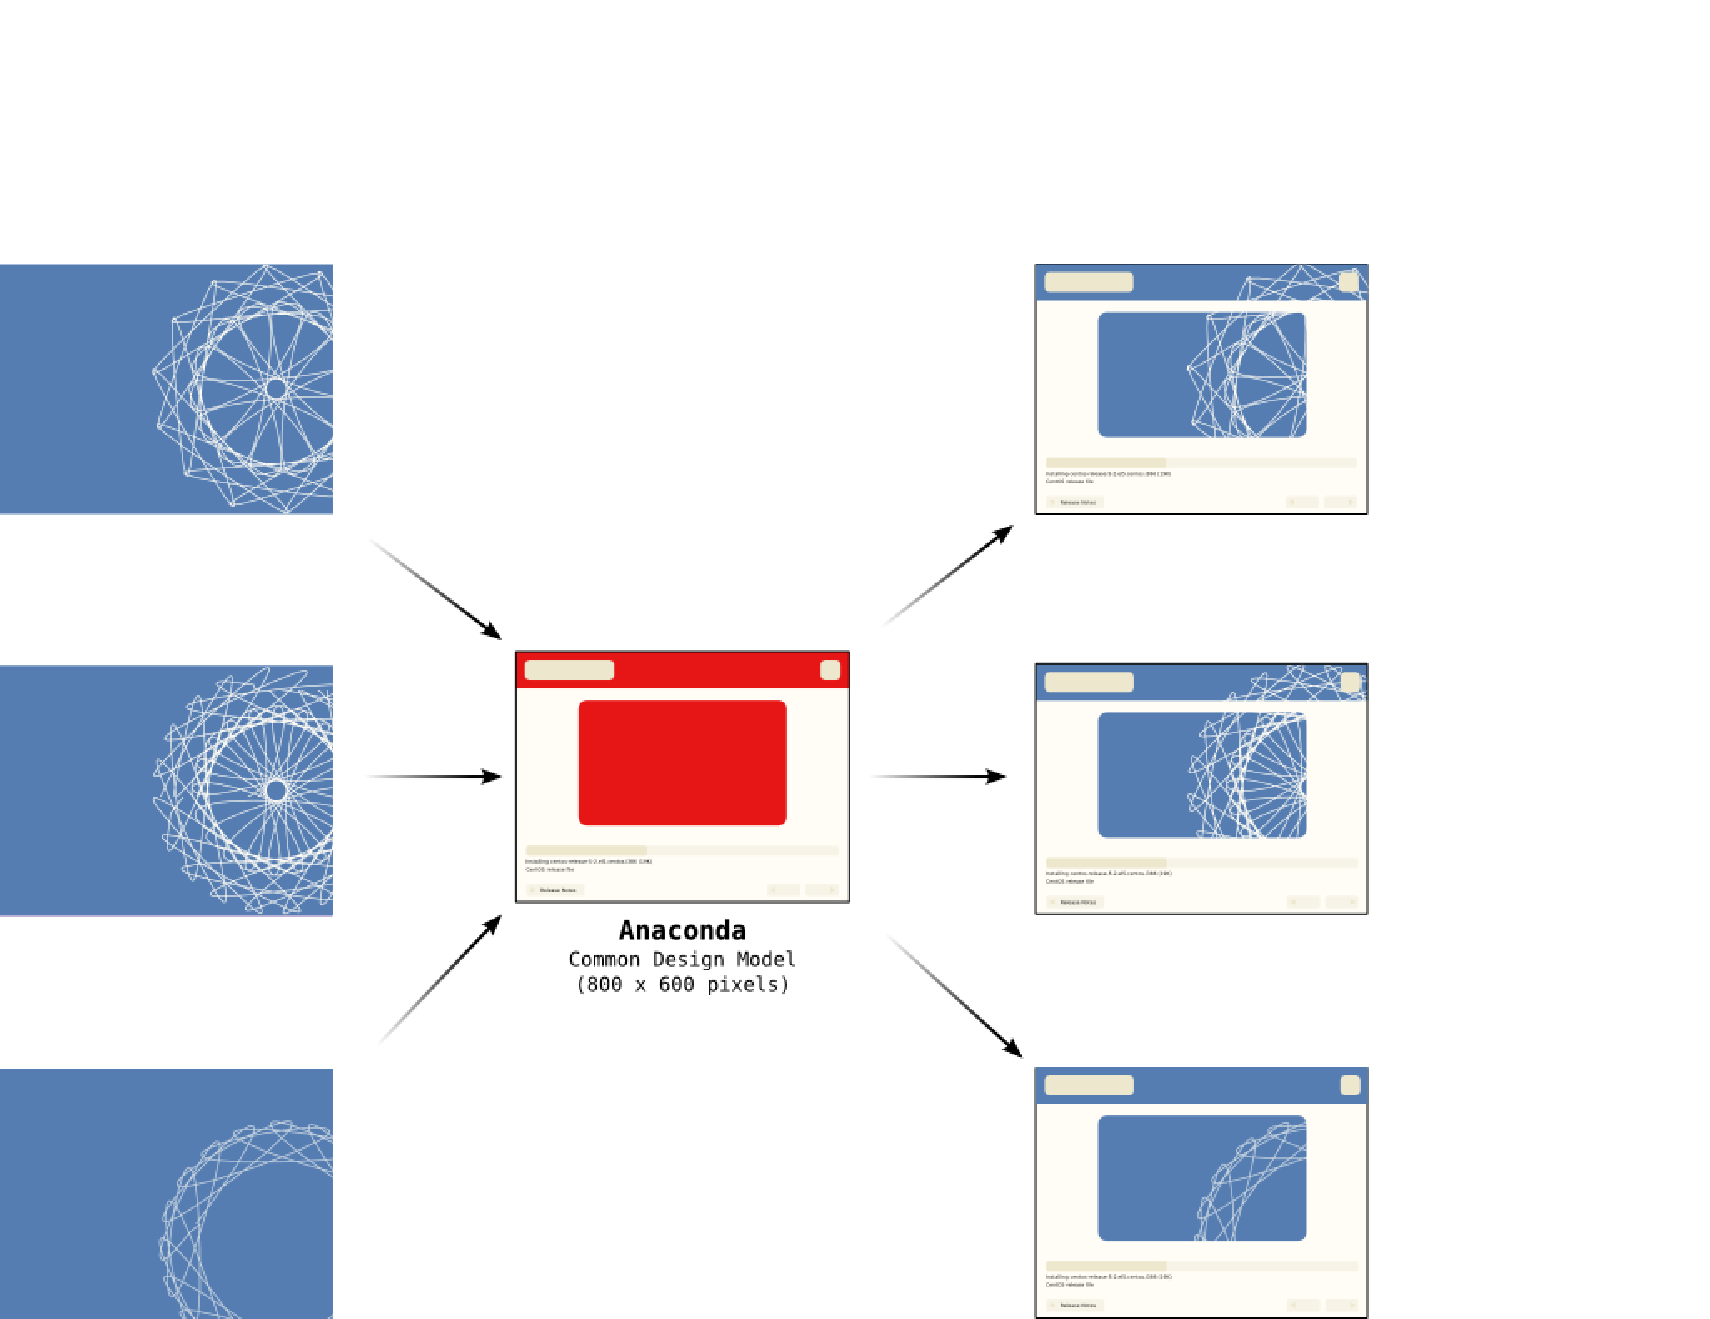
\includegraphics[width=0.8\textwidth]{%
   /home/centos/artwork/trunk/Identity/Models/Img/en/Corporate/common-design-model-fig1.pdf}}
\end{center}
\caption{Anaconda theme model producing three different visual
styles.}
\end{figure}

\begin{figure}
\begin{center}
\fbox{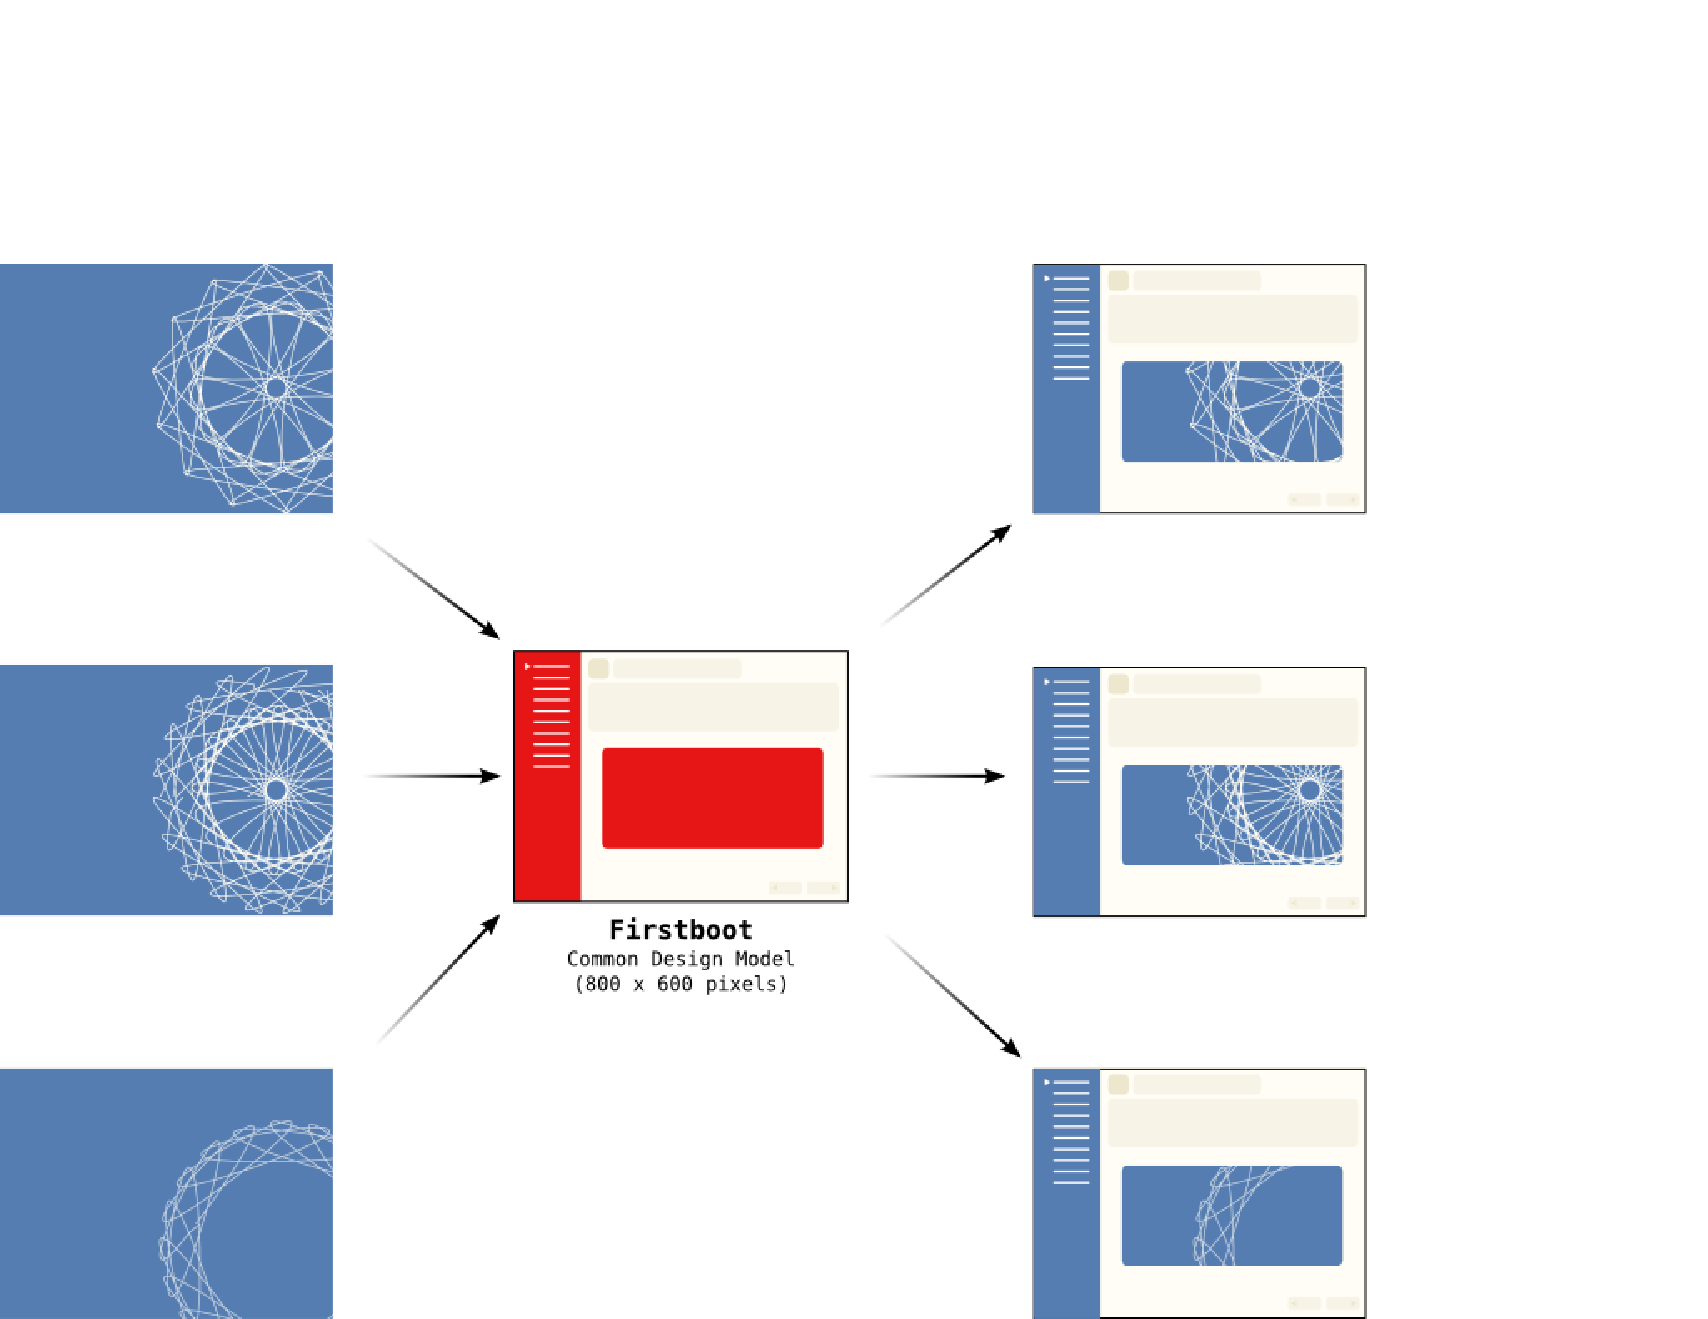
\includegraphics[width=0.8\textwidth]{%
   /home/centos/artwork/trunk/Identity/Models/Img/en/Corporate/common-design-model-fig2.pdf}}
\end{center}
\caption{Firstboot theme model producing three different visual
styles.}
\end{figure}

% ------------------------------------------------------------
\section{Theme Motifs}
\hypertarget{sec:Concepts:Identity:Themes:Motifs}{}
\label{sec:Concepts:Identity:Themes:Motifs}

\begin{description}
\item[framework:] trunk/Identity/Themes/Motifs/
\end{description}

\noindent Here is where the themes' artistic motifs are produced. The
artistic motif is a graphic design used as common pattern to connect
all CentOS Project's visual manifestations inside the same theme.

Inside the framework location above, artistic motifs are organized by
names inside the standard file structure illustrated in
\autoref{fig:Concepts:Identity:Themes:Motifs:Default} and
\autoref{fig:Concepts:Identity:Themes:Motifs:Alternative}.

\begin{figure}[!hbp]
\hrulefill
\begin{verbatim}
trunk/Identity/Themes/
|-- Motifs
|   |-- Modern              <-- theme name.
|   |   |-- Backgrounds
|   |   |-- Distro
|   |   |   |-- Anaconda
|   |   |   |   |-- Header
|   |   |   |   |-- Progress
|   |   |   |   |-- Prompt
|   |   |   |   `-- Splash
|   |   |   |-- BootUp
|   |   |   |   |-- Firstboot
|   |   |   |   |-- GDM
|   |   |   |   |-- GRUB
|   |   |   |   |-- GSplash
|   |   |   |   |-- KDM
|   |   |   |   |-- KSplash  
|   |   |   |   |-- RHGB
|   |   |   |   `-- Plymouth
|   |   |   `-- Desktop
|   |   |-- Info
|   |   |-- Palettes
|   |   |-- Promo
|   |   |-- Screenshots
|   |   `-- Web
|   |-- ... more theme names.
\end{verbatim}
\hrulefill
\caption{Theme motifs default structure.%
   \label{fig:Concepts:Identity:Themes:Motifs:Default}}
\end{figure}

\begin{figure}[!hbp]
\hrulefill
\begin{verbatim}
trunk/Identity/Themes/
|-- Motifs
|   |-- TreeFlower          <-- theme name.
|   |   |-- Backgrounds
|   |   |-- Distro
|   |   |   |-- BootUp
|   |   |   |   |-- Firstboot
|   |   |   |   |-- GDM
|   |   |   |   |-- GRUB
|   |   |   |   |-- GSplash
|   |   |   |   |-- KDM
|   |   |   |   |-- KSplash  
|   |   |   |   |-- RHGB
|   |   |   |   `-- Plymouth
|   |   |   `-- Desktop
|   |   |-- Info
|   |   |-- Palettes
|   |   |-- Screenshots
|   |-- ... more theme names.
\end{verbatim}
\hrulefill
\caption{Theme motifs alternative structure.%
   \label{fig:Concepts:Identity:Themes:Motifs:Alternative}}
\end{figure}

When designing artistic motifs for CentOS, consider the following
recommendations:

\begin{itemize}

\item Give a unique (case-sensitive) name to your Motif. This name is
used as value wherever theme variable (\$THEME) or translation marker
(\texttt{=THEME=}) is.  Optionally, you can add a description about
inspiration and concepts behind your work.

\item Use the location trunk/Identity/Themes/Motifs/\$THEME/ to store
your work. If it doesn't exist create it. Note that this require you
to have previous commit access in CentOS Artwork Repository.

\item The CentOS Project is using the blue color (\texttt{\#204c8d})
as base for its corporate visual identity. Use the CentOS Project's
base corporate color as much as possible in your artistic motif
designs.

\item Try to make your design fit one of the
``\hyperlink{sec:Concepts:Identity:Themes:Models}{Theme Models}''
(\autoref{sec:Concepts:Identity:Themes:Models}).

\item Feel free to make your art enterprise-level and beautiful.

\item Add the following information on your art work (both in a visible
design area, and inside Inkscape's document metadata section wherever
it be possible):

\begin{itemize}

\item The name (or logo) of your artistic motif.

\item The copyright sentence: \texttt{Copyright (C) YEAR YOURNAME}

\item The license under which the work is released. All CentOS Art
works are released under
\href{http://creativecommons.org/licenses/by-sa/3.0/}{Creative Common
Share-Alike License 3.0}
(\href{http://creativecommons.org/licenses/by-sa/3.0/}{http://creativecommons.org/licenses/by-sa/3.0/}).

\end{itemize}

\end{itemize}
% ------------------------------------------------------------
\section{Theme Palettes}
\hypertarget{sec:Concepts:Identity:Themes:Palettes}{}
\label{sec:Concepts:Identity:Themes:Palettes}

\begin{description}
\item[framework:] turnk/Identity/Themes/Motifs/\$THEME/Palettes/\\
\end{description}

\noindent Here is where graphic designers define theme palettes for
color-limited art works. Theme palettes contain the color information
that rendering functions need, in order to produce images with color
limitations.  Theme palettes contain theme's unique color information.
\autoref{tab:Concepts:Identity:Themes:Palettes:Files}.

% ------------------------------------------------------------
\section{Theme Palettes Creation}
\hypertarget{sec:Concepts:Identity:Themes:Palettes:Creation}{}
\label{sec:Concepts:Identity:Themes:Palettes:Creation}

Theme palettes are based on art works' specific color information you
are creating palettes for. As we write this section, there are two art
works that require color limitations. They are Grub and Syslinux art
works.

This section describes a generic procedure you can use to create theme
palettes for art works which need to be produced with color
limitations.

\begin{enumerate}

\item As first step, you need to produce a PNG file with the final
design of that art work you are creating palettes for.  You can do
this by using the \texttt{render.sh} script available in the art
work's identity framework.

\item Secondly, you need to generate the limited color information for
that PNG file the three different file formats (See
\autoref{tab:Concepts:Identity:Themes:Palettes:Files}). You can do
this by using the Gimp as described below: 

\begin{table}[!hbp]
\center
\begin{tabular}{ll}
\hline
\textbf{File} & \textbf{Description}\\
\hline
\texttt{.gpl} & Gimp palette files.\\
\texttt{.ppm} & Portable Pixel Map palette files.\\
\texttt{.hex} & Hexadecimal auxiliar palette files.\\
\hline
\end{tabular}
\caption{Palette file types.% 
   \label{tab:Concepts:Identity:Themes:Palettes:Files}}
\end{table}

\end{enumerate}

To create the \texttt{.gpl} file:

\begin{enumerate}

\item Open the Gimp (\textit{Applications / Graphics / The Gimp}).

\item Open the PNG format file you want to generate the limited color
information for (\textit{File / Open ...}).

\item Index the image (\textit{Image / Mode / Indexed...}).  This will
open the window ``Indexed Color Conversion''. Use this window to
``Generate optimum palette'' by setting the maximum number of colors
you want to have in the final indexed image. In this window, by the
default, Gimp has set 255 as the maximum number of colors, you should
change this value to fit the art work color limitation requirements
(i.e. 14 colors for Grub's splash, and 16 colors for Syslinux splash,
etc.). Another option you can play with is ``Color dithering'' at the
window's bottom, particularly the ``Floyd-Steinberg (reduced color
dithering)'' option which seems to archive the best results.

\item At this point you have reduced color information and indexed the
image. This let you save the color information as a Gimp palette file
(.gpl) for further using. 

To export the color information as Gimp palette you need to open the
palette window (\textit{Ctrl+P}) and go to the action ``Import
Palette...'' inside ``Palettes Menu''. This will open the window
``Import Palette''. In this window you need to specify the source from
where you will retrive color information and the name of the palette
file. Use ``Image'' as source to create your palette and the
appropriate name (e.g., \texttt{centos-\$themename-grub}).\footnote{in
\texttt{centos-\$themename-grub} file name, the \texttt{\$themename}
part is the theme's name you are working on (e.g., Modern, TreeFlower,
etc.) for Grub's palette, \texttt{centos-\$themename-syslinux} for
Syslinux palette, etc.}

\end{enumerate}

To create the \texttt{.ppm} file:

\begin{enumerate}

\item Use the Gimp to create a new image (\textit{Ctrl+N}) of 16 x 1
pixels of dimension.  That is 16 pixels width and 1 pixel height.
      
\item That is a rather small image so you problably want to zoom it in
to better see what you are doing. In a 1024x768 screen resolution,
zoom the 16 x 1 pixel image to 4500\% makes things clear enough. If
you are using a different screen resolution you probably need to zoom
in to a different value. 

\item Now it's time to fill up the empty image with the color
information we created previously. You do this using the pen tool
(\textit{N}) with a 1x1 brush (\textit{Shit+Ctrl+B}). At this point it
is a good time to open the ``Palette Editor'' window and use the Gimp
palette file with the color information we created (\textit{Ctrl+P /
doble click on the palette file}).

\begin{quote} 

\textbf{Caution!:} If you are creating \texttt{.ppm} palettes for
Anaconda prompt (syslinux), the order used to set the color
information is relevant. Relevant values in the image are positions: 0
and 7.  Position 0 is used as background color, which is black
(\texttt{\#000000}) generally and position 7 is used as forground
color, which is white (\texttt{\#ffffff}) generally. This, in order to
grant the highest contrast.  See
\autoref{fig:Concepts:Identity:Themes:Palettes:Syslinux}.

\end{quote}
      
\end{enumerate}

To create the (\texttt{.hex}) file:

\begin{enumerate}

\item Create a plain text file and put the hexadecimal color
information and its index position defined in \texttt{.ppm} palette
inside the file, one definition by line.  The format used to create
the \texttt{.hex} file is \texttt{\#rrbbgg=i \dots}.  Where
\texttt{\#rrggbb=i} indicates that the color \texttt{\#rrggbb} (hex)
should be assigned index i (decimal).

\begin{quote}
\textbf{Caution!:} In order to produce Anaconda prompt (syslinux)
images correctly, both \texttt{.hex} and \texttt{.ppm} color and index
information should match.
\end{quote}

\end{enumerate}

\begin{figure}[!hbp]
\begin{center}
\fbox{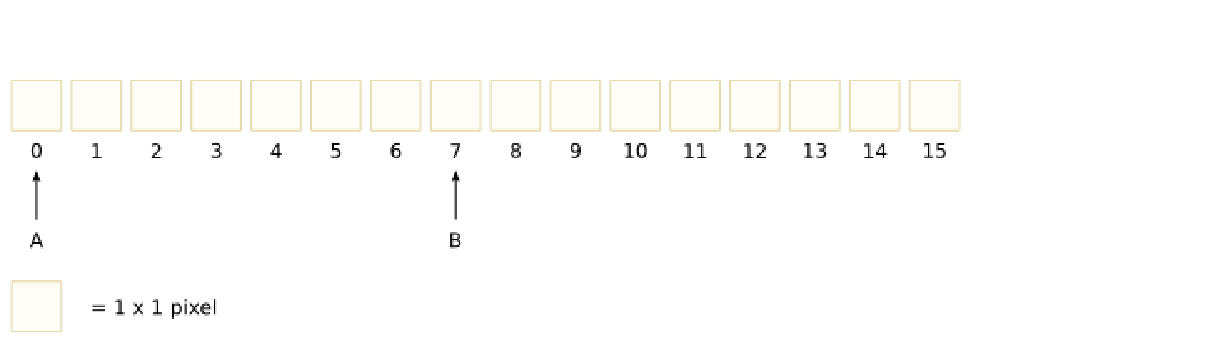
\includegraphics[width=0.8\textwidth]{%
   /home/centos/artwork/trunk/Identity/Models/Img/en/Distro/Anaconda/Prompt/syslinux-palette.pdf}}
\end{center}
\caption{Palette's background (A) and forground (B) color position.%
    \label{fig:Concepts:Identity:Themes:Palettes:Syslinux}}
\end{figure}

% ------------------------------------------------------------
\section{Theme File Structure}
\hypertarget{sec:Concepts:Identity:Themes:Files}{}
\label{sec:Concepts:Identity:Themes:Files}

Inside CentOS Artwork Repository, each theme has a name and a
directory for it. Inside each theme directory, the CentOS Project
visual style is organized in the directories: Distro, Info, Palettes,
Promo, Screenshots, and Web. 

% ------------------------------------------------------------
\subsection{The \texttt{Distro} Directory}
\hypertarget{sec:Concepts:Identity:Themes:Files:Distro}{}
\label{sec:Concepts:Identity:Themes:Files:Distro}

Here is where image files controlling CentOS Distribution visual style
are produced. 

\begin{figure}[!hbp]
\hrulefill
\begin{verbatim}
turnk/Identity/Themes/Motifs/$THEME/Distro/
|-- Anaconda
|   |-- Header
|   |-- Progress
|   |-- Prompt
|   `-- Splash
|-- BootUp
|   |-- Firstboot
|   |-- GDM
|   |-- GRUB
|   |-- GSplash
|   |-- KDM
|   |-- KSplash
|   `-- RHGB
`-- Desktop
\end{verbatim}
\hrulefill
\caption{The CentOS distribution theme structure.}
\end{figure}

% ------------------------------------------------------------
\subsection{The \texttt{Palettes} Directory}
\hypertarget{sec:Concepts:Identity:Themes:Files:Palettes}{}
\label{sec:Concepts:Identity:Themes:Files:Palettes}

Here is where theme's palettes are sotred. Palettes are used to
automate image rendering in cases where a limited amount of color need
to be specified. Before you could render color-limited art works (e.g.
Grub, and Syslinux), you need to create their color-limited palettes
first. See
``\hyperlink{sec:Concepts:Identity:Themes:Palettes:Creation}{Theme
Palette Creation}''
(\autoref{sec:Concepts:Identity:Themes:Palettes:Creation}).

% ------------------------------------------------------------
\subsection{The \texttt{Promo} Directory}
\hypertarget{sec:Concepts:Identity:Themes:Files:Promo}{}
\label{sec:Concepts:Identity:Themes:Files:Promo}

Here is where image files controlling CentOS promotion visual style
are produced.

% ------------------------------------------------------------
\subsection{The \texttt{Screenshots} Directory}
\hypertarget{sec:Concepts:Identity:Themes:Files:Screenshots}{}
\label{sec:Concepts:Identity:Themes:Files:Screenshots}

Here is where theme's screenshots are stored. The purpose of this
directory is to collect theme's implementation graphical history
through time. Inside this directory you can have distribution
screenshots, web sites screenshtos, and promotion screenshots. If
theme has been implemented out of computers like would be the case of
events, stands, etc. those photos can be added here too, in the
promotion screenshot section.

% ------------------------------------------------------------
\subsection{The \texttt{Web} Directory}
\hypertarget{sec:Concepts:Identity:Themes:Files:Web}{}
\label{sec:Concepts:Identity:Themes:Files:Web}

Here is where image files controlling CentOS Web sites visual style
are produced.

   % Part   : Concepts
% Chapter: Corporate Identity
% ------------------------------------------------------------
% $Id: icons.tex 6023 2010-06-27 10:09:48Z al $
% ------------------------------------------------------------

\section{Icons}
\hypertarget{sec:Concepts:Identity:Icons}{}
\label{sec:Concepts:Identity:Icons}

\begin{description}
\item[framework:] trunk/Identity/Icons/
\end{description}


   % Part   : Concepts
% Chapter: Corporate Identity
% ------------------------------------------------------------
% $Id: models.tex 6023 2010-06-27 10:09:48Z al $
% ------------------------------------------------------------

\section{Models}
\hypertarget{sec:Concepts:Identity:Models}{}
\label{sec:Concepts:Identity:Models}

\begin{description}
\item[framework:] trunk/Identity/Models/
\end{description}

\noindent Here is where you find design models. Design models are
representative images used to illustrate key components inside a
specific design. Design models are frequently used to make
documentation clearer. 

When designing models, try to make them language independent so they
can be reused in differet language documents. For example, you can use
letters or numbers to identify areas in the model and later use the
figure's caption to describe the meaning of those letters and numbers,
respectively.  

   % Part   : Concepts
% Chapter: Corporate Identity
% ------------------------------------------------------------
% $Id: widgets.tex 6023 2010-06-27 10:09:48Z al $
% ------------------------------------------------------------

\section{Widgets}
\hypertarget{sec:Concepts:Identity:Widgets}{}
\label{sec:Concepts:Identity:Widgets}

\begin{description}
\item[framework:] trunk/Identity/Widgets/
\end{description}


\chapter{Translations}
   \hypertarget{cha:Concepts:Translations}{}
   \label{cha:Concepts:Translations}
   % ------------------------------------------------------------
% $Id$
% ------------------------------------------------------------
\begin{figure}
\hrulefill
\begin{verbatim}
trunk/Translations/Identity/Themes/Distro/Anaconda/Header/
|-- 3
|   `-- anaconda_header.sed
|-- 4
|-- 5
|-- ... more major releases
|-- render.sh
`-- tpl
    `-- anaconda_header.sed
\end{verbatim}
\hrulefill
\caption{Anaconda header translation framework.%
   \label{fig:Distribution:Anaconda:Header:Translations}}
\end{figure}

% ------------------------------------------------------------ 
\subsection{Translation Markers}
\hypertarget{sec:Distribution:Anaconda:Header:Translations:Markers}{}
\label{sec:Distribution:Anaconda:Header:Translations:Markers}

\begin{itemize}
\item \texttt{=VERSION=}: Major release number of CentOS distribution.
\end{itemize}



\chapter{Manuals}
   \hypertarget{cha:Concepts:Manuals}{}
   \label{cha:Concepts:Manuals}
   % Part   : Concepts
% Chapter: Manuals
% ------------------------------------------------------------
% $Id: manuals.tex 6191 2010-08-02 02:36:14Z al $
% ------------------------------------------------------------

\begin{description}
\item[framework:] trunk/Manuals/
\end{description}

\noindent This chapter describes the CentOS Artwork Repository User
Guide.  The CentOS Artwork Repository User Guide is the book you are
reading right now. The main goals of this book is helping you to
understand how CentOS Artwork Repository works, and what you can do to
get the best of it.  It is also an excuse for you to join us and help
improving it.

\section{Structure}

Inside CentOS Artwork Repository, documentation is conceived using
\LaTeX's book class. Instead of having the entire document in a single
file, information has been spread in separated files under Manuals
framework structure. The Manuals framework structure is illustrated in
\autoref{fig:Concepts:Manuals:Structure} and described in
``\hyperlink{sec:Concepts:Manuals:Files}{Relevant Files}'' (see
\autoref{sec:Concepts:Manuals:Files}) and
``\hyperlink{sec:Concepts:Manuals:Directories}{Relevant Directories}''
(see \autoref{sec:Concepts:Manuals:Directories}).

\begin{figure}[!hbp]
\hrulefill
\begin{verbatim}
trunk/Manuals/
|-- Concepts
|   |-- CentOS
|   |-- Frameworks
|   |-- Identity
|   `-- ...
|-- Distribution
|   |-- Anaconda
|   |   |-- Firstboot
|   |   |-- Header
|   |   |-- Progress
|   |   `-- ...
|   |-- Backgrounds
|   |-- BootUp
|   |   |-- GDM
|   |   |-- GRUB
|   |   `-- ...
|   `-- Release
|-- Licenses
|-- Translations
|-- Workstation
|-- convenctions.tex
|-- repository.aux
|-- repository.lof
|-- repository.log
|-- repository.lot
|-- repository.out
|-- repository.pdf
|-- repository.tex
`-- repository.toc
\end{verbatim}
\hrulefill
\caption{Manuals framework structure.%
   \label{fig:Concepts:Manuals:Structure}}
\end{figure}

\section{Writing Style}

When writing for CentOS Artwork Repository User Guide, keep in mind
the following quote taken from the online ``BBC News Styleguide'':
---The key to good writing is \textbf{simple thoughts simply
expressed}.  Use short sentences and short words.  Anything which is
confused, complicated, poorly written or capable of being
misunderstood risks losing the listener or viewer, and once you have
done that, you might just as well not have come to work---.

If you need to express complicated ideas, try to split them out in
smaller and simpler ideas as much as possible. If you consider it
appropriate, try to use
``\hyperlink{sec:Concepts:Identity:Models}{Design Models}'' (see
\autoref{sec:Concepts:Identity:Models}) to illustrate your thoughts.

\subsection{Cross References}

When you create \LaTeX's cross references, you need to define targets
and links.  Targets are the specific locations in the document that
links point to.  In \LaTeX, these cross reference targets and links
can be defined in many ways, so we need to standardize the way we use
inside CentOS Artwork Repository User Guide to make it look uniform
and easy to read.

Inside CentOS Artwork Repository User Guide, cross references look
like illustrated in
\autoref{fig:Concepts:Manuals:CrossRef:Presentation}.  Cross reference
targets are defined as illustrated in
\autoref{fig:Concepts:Manuals:CrossRef:Targets}, and links to those
targets are defined as illustrated in
\autoref{fig:Concepts:Manuals:CrossRef:Links}. 

Note that we use both \texttt{hypertarget} and \texttt{label} commands
to define targets, and \texttt{hyperlink} and \texttt{autoref} to
define links.  With \texttt{hyperlink} we create long text links
---usefull when reading in the coputer---, and with \texttt{autoref}
we create numbered links ---usefull when reading in a printed copy---.

\begin{figure}[!hbp]
\hrulefill
\begin{flushleft}
\dots you can find more information in
``\hyperlink{sec:Concepts:Identity:Brands}{Logos}'' (see
\autoref{sec:Concepts:Identity:Brands}), specifically in
\hyperlink{sec:Concepts:Identity:Brands:Logos}{the horizontal version} (see
\autoref{sec:Concepts:Identity:Brands:Logos}).
\end{flushleft}
\hrulefill
\caption{Cross reference link presentation.%
   \label{fig:Concepts:Manuals:CrossRef:Presentation}}
\end{figure}

\begin{figure}[!hbp]
\hrulefill
\begin{verbatim}
\part{Concepts}
...
\chapter{The CentOS Logo}
\hypertarget{sec:Concepts:Logo}{}
\label{sec:Concepts:Logo}
...
\section{Horizontal}
\hypertarget{sec:Concepts:Identity:Brands}{}
\label{sec:Concepts:Identity:Brands}
...
\end{verbatim}
\hrulefill
\caption{\LaTeX's definition for cross reference targets.%
   \label{fig:Concepts:Manuals:CrossRef:Targets}}
\end{figure}

\begin{figure}[!hbp]
\hrulefill
\begin{verbatim}
\dots you can find more information in
``\hyperlink{sec:Concepts:Identity:Brands}{The CentOS Logo}'' 
(see \autoref{sec:Concepts:Identity:Brands}), specifically in
\hyperlink{sec:Concepts:Identity:Brands:Logos}{the horizontal version} 
(see \autoref{sec:Concepts:Identity:Brands:Logos}).
\end{verbatim}
\hrulefill
\caption{\LaTeX's definition for cross reference links.%
   \label{fig:Concepts:Manuals:CrossRef:Links}}
\end{figure}

\subsection{Figures}

Inside CentOS Artwork Repository User Guide, illustrations (i.e.
images, framework structures, source code, commands, etc.) are shown
using \LaTeX's \texttt{figure} environment. An example of
\texttt{figure} environment definition is illustrated in
\autoref{fig:Concepts:Manuals:Figures}.  More information about
\LaTeX's \texttt{figure} environment can be found in \LaTeX's info
manual. To read the \LaTeX's info manual, execute in your terminal the
command: \texttt{info latex}.

\begin{figure}[!hbp]
\hrulefill
\begin{verbatim}
\begin{figure}[!hbp]
\hrulefill
...
\hrulefill
\caption{... .%
   \label{fig:...}}
\end{figure}
\end{verbatim}
\hrulefill
\caption{\LaTeX's definition for \texttt{figure} environment.%
   \label{fig:Concepts:Manuals:Figures}}
\end{figure}

\subsection{Tables}

Inside CentOS Artwork Repository User Guide, tabular information (i.e.
translation markers, etc.) is shown using \LaTeX's \texttt{table}
environment. An example of \texttt{table} environment definition is
illustrated in \autoref{fig:Concepts:Manuals:Tables}.  More
information about \LaTeX's \texttt{table} environment can be found in
\LaTeX's info manual. To read the \LaTeX's info manual, execute in
your terminal the command: \texttt{info latex}.

\begin{figure}[!hbp]
\hrulefill
\begin{verbatim}
\begin{table}[!hbp]
\centering
\begin{tabular}[pos]{cols}
\hline
...
\hline
\end{tabular}
\caption{... .%
   \label{tab:...}}
\end{table}
\end{verbatim}
\hrulefill
\caption{\LaTeX's definition for \texttt{table} environment.%
   \label{fig:Concepts:Manuals:Tables}}
\end{figure}

\section{Relevant Files}
\hypertarget{sec:Concepts:Manuals:Files}{}
\label{sec:Concepts:Manuals:Files}

\subsection{repository.tex}

The \texttt{repository.tex} file is the main book's file. Here is
where you define specific book information like class, title, authors,
etc.  Inside \texttt{repository.tex} you organize chapters and load
their sections.

\subsection{introduction.tex} 

The \texttt{Introduction.tex} file introduces a specific artwork
component: what it does, where and when it appears in, etc.

\subsection{framework.tex} 

The \texttt{rramework.tex} file describes how to interact with a
specific artwork component: where to find the artwork component inside
CentOS Artwork Repository, how to render their images, how to render
their translations, their specific translation markers, etc.

\subsection{rebranding.tex} 

The \texttt{rebranding.tex} file describes how to rebrand a specific
artwork component: where to find the arwork component inside CentOS
Distribution, related packages you need to modify, etc.

\section{Relevant Directories}
\hypertarget{sec:Concepts:Manuals:Directories}{}
\label{sec:Concepts:Manuals:Directories}

\subsection{Concepts}

The \texttt{Concepts} directory organizes chapters related to
``Concepts'' part.  Files in this directory describe concepts used
inside CentOS Artwork Repository.

\subsection{Workstation} 

The \texttt{Workstation} directory organizes chapters related to
``Preparing Your Workstation'' part. Files in this directory describe
actions (i.e. installation and configuration) you need to do before
using CentOS Artwork Repository. 

\subsection{Distribution} 

The \texttt{Distribution} directory organizes chapters releated to
``Distribution'' part. This part gets its attention into the different
artwork components of CentOS Distribution, using a subdirectory
structure to organize them and the files \texttt{introduction.tex},
\texttt{framework.tex}, and \texttt{rebranding.tex} to describe them.

\subsection{Licenses} 

The \texttt{Licenses} directory organizes licenses used in this book.

\section{Revisions}
\hypertarget{sec:Concepts:Manuals:Revisions}{}
\label{sec:Concepts:Manuals:Revisions}

Revisions are a way of organizing changes committed to CentOS Artwork
Repository User Guide. Revisions have the format ``Revision M.N'',
where M is the major revision number, and N is the update revision
number.  Revision update number (N) may increase by one every month to
release that month's changes.  Once the six month cycle is reached,
major revision number (M) is increased by one and update revision
number (N) is reset to 0.

\section{Export to PDF}

To produce the file \texttt{repository.pdf}, you need to get inside
the Manual's framework and execute the command:

\begin{quote}
\texttt{pdflatex repository.tex}
\end{quote}


\chapter{Scripts}
   \hypertarget{cha:Concepts:Scripts}{}
   \label{cha:Concepts:Scripts}
   % Part   : Distribution
% Chapter: Anaconda Header
% Section: Scripts
% ------------------------------------------------------------
% $Id$
% ------------------------------------------------------------
\begin{itemize}
\item trunk/Scripts/Identity/Themes/Distro/Anaconda/Header/
\end{itemize}


\chapter{Rebranding}
   \hypertarget{cha:Concepts:rebranding}{}
   \label{cha:Concepts:rebranding}
   % Part   : Concepts
% Chapter: Rebranding
% ------------------------------------------------------------
% $Id: rebranding.tex 6191 2010-08-02 02:36:14Z al $
% ------------------------------------------------------------

To comply with upstream redistribution policy, the CentOS Project
removes all upstream brands and artworks from CentOS Distribution. The
CentOS Project has its own brand and its own artwork. The CentOS Brand
and CentOS Artwork are what the CentOS Project uses in CentOS
Distribution. 

The action of removing upstream brands and artworks and add CentOS
brands and artworks is what we call rebranding.

CentOS Brands and artworks are organized inside CentOS Artwork
Repository.  The CentOS Artwork Repository is maintain by CentOS
Artwork SIG which is formed by CentOS Community People.

\section{General Suggestions}

\begin{itemize}

\item Use original names as much as possible. Do not rename original
file names if you don't need to.

\end{itemize}



\part{Preparing Your Workstation}

\chapter{Installation}
   \hypertarget{cha:Workstation:Installation}{}
   \label{cha:Workstation:Installation}
   % Part   : Preparing Your Workstation
% Chapter: Installation
% ------------------------------------------------------------
% $Id: installation.tex 6191 2010-08-02 02:36:14Z al $
% ------------------------------------------------------------

This chapter describes tools you need to have installed in your CentOS
workstation before using CentOS Artwork Repository.

\section{Subversion}

Subversion is a version control system, which allows you to keep old
versions of files and directories (usually source code), keep a log of
who, when, and why changes occurred, etc., like CVS, RCS or
SCCS.\footnote{More documentation about Subversion and its tools,
including detailed usage explanations of the svn, svnadmin, svnserve
and svnlook programs, historical background, philosophical approaches
and reasonings, etc., can be found at
\url{http://svnbook.red-bean.com/.}} 

To install Subversion client tools in your workstation you can use the
following command:

\begin{quote}
yum install subversion
\end{quote}

\section{Inkscape}

Inkscape is a GUI editor for Scalable Vector Graphics (SVG) format
drawing files, with capabilities similar to Adobe Illustrator,
CorelDraw, Visio, etc. Inkscape features include versatile shapes,
bezier paths, freehand drawing, multiline text, text on path, alpha
blending, arbitrary affine transforms, gradient and pattern fills,
node editing, SVG-to-PNG export, grouping, layers, live clones, and
more.

Note that Inkscape is not inside CentOS Distribution, so you need to
configure a third party repository like RPMForge or EPEL to install
Inkscape.  Installation of a third party repositories inside CentOS
Distribution is described in the following URL:

\begin{quote}
\url{http://wiki.centos.org/AdditionalResources/Repositories}
\end{quote}

Once you have configured the third party repository you can install
Inkscape using the following command:

\begin{quote}
yum install inkscape
\end{quote}

\section{ImageMagick}

ImageMagick is a free software suite for the creation, modification
and display of bitmap images. It can read, convert and  write images
in a large variety of formats. Images can be cropped, colors can be
changed, various effects can be applied, images can  be rotated  and
combined,  and text, lines, polygons, ellipses and Bézier curves can
be added to images and stretched and rotated.

To install ImageMagick in your workstation you can run the following
command:

\begin{quote}
yum install ImageMagick
\end{quote}

\section{Netpbm}

Netpbm is a toolkit for manipulation of graphic images, including
conversion of images between a variety of different formats.  There
are over 300 separate tools in the package including converters for
about 100 graphics formats.

To install Netpbm in your workstation you can run the following
command:

\begin{quote}
yum install netpbm\{-progs\}
\end{quote}

\section{Syslinux}

Syslinux is a suite of bootloaders, currently supporting DOS FAT
filesystems, Linux ext2/ext3 filesystems (EXTLINUX), PXE network boots
(PXELINUX), or ISO 9660 CD-ROMs (ISOLINUX).  It also includes a tool,
MEMDISK, which loads legacy operating systems from these media.  The
package \texttt{syslinux} provides the programs \texttt{ppmtolss16}
and \texttt{lss16toppm} which are used to produce Anaconda Prompt
images. The \texttt{ppmtolss16} Perl program also includes the file
format specification.

To install Syslinux in your workstation you can run the following
command:

\begin{quote}
yum install syslinux
\end{quote}

\section{GNU Image Manipulation Program}

GNU Image Manipulation Program (GIMP) is used to manipulate images
inside CentOS Artwork Repository.  

To install GIMP in your workstation you can run the following command:

\begin{quote}
yum install gimp
\end{quote}

\section{GNU Core Utilities}

The GNU core utilities are a set of tools commonly used in shell
scripts.

To install the GNU core utilities in your workstation you can run the
following command:

\begin{quote}
yum install core-utils
\end{quote}

\section{\LaTeX}

\LaTeX\ is a document preparation system implemented as a macro
package for Donald E.  Knuth's \TeX\ typesetting program. The \LaTeX\
command typesets a file of text using the \TeX\ program and the LaTeX
Macro package for \TeX.  To be more specific, it processes an input
file containing the text of a document with interspersed commands that
describe how the text should be formatted. 

To install \LaTeX\ in your workstation you can run the following
command:

\begin{quote}
yum install tetex-\{latex,fonts,doc,xdiv,dvips\}
\end{quote}


\chapter{Configuration}
   \hypertarget{cha:Workstation:Configuration}{}
   \label{cha:Workstation:Configuration}
   % Part   : Preparing Your Workstation
% Chapter: Configuration
% ------------------------------------------------------------
% $Id: configuration.tex 6191 2010-08-02 02:36:14Z al $
% ------------------------------------------------------------

This chapter describes configurations you need to set up before using
CentOS Artwork Repository.

\section{Firewall}

The CentOS Artwork Repository lives on the following URL:

\begin{quote}
https://projects.centos.org/svn/artwork/
\end{quote}

To reach this location you need to have Internet access and be sure no
rule in your firewall is denying this site. Note that the URL uses the
SSL protocol (port 443).

\section{Subversion Behind Squid}

Sometimes it is convenient to proxy Subversion client's requests
through a proxy-cache server like Squid. In cases like this, the Squid
proxy server is in the middle between you and CentOS Artwork
Repository. If you want to proxy Subversion client's requests through
Squid proxy-cache server, you need to configure your Subversion client
and your Squid proxy server to do so.

\subsection{Subversion Client Configuration}

Subversion client needs to be configured to send requests to your
Squid proxy-cache server. This configuration takes place in the file
\texttt{$\sim$/.subversion/servers}.

\subsection{Squid Server Configuration}

Squid proxy-cache server needs to be configured to accept the
extension methods \texttt{REPORT MERGE MKACTIVITY CHECKOUT MKCOL}.
This configuration takes place in the file
\texttt{/etc/squid/squid.conf}, specifically in the configuration tag
illustrated in \autoref{fig:Workstation:Configuration:Squid}.

\begin{figure}[!hbp]
\hrulefill
\begin{verbatim}
#  TAG: extension_methods
#       Squid only knows about standardized HTTP request methods.
#       You can add up to 20 additional "extension" methods here.
#
#Default:
# none
extension_methods REPORT MERGE MKACTIVITY CHECKOUT MKCOL
\end{verbatim}
\hrulefill
\caption{Squid configuration to proxy Subversion client's requests.%
   \label{fig:Workstation:Configuration:Squid}}
\end{figure}

\section{Working Copy}

A Subversion working copy is an ordinary directory tree on your local
system, containing a collection of files (i.e.  Translations, Designs,
Manuals, and Scripts). You can edit these files however you wish. Your
working copy is your own private work area: Subversion will never
incorporate other people's changes, nor make your own changes
available to others, until you explicitly tell it to do so.  You can
even have multiple working copies of the same project.\footnote{Even
this is basically correct, doing so when using CentOS Artowrk
Repository can bring some confusion when executing scripts. Presently,
only one absolute path can be defined as absolute path for scripts'
execution.  You can have as many working copies of CentOS Artwork
Repository as you want but scripts will be executed from just one
working copy absolute path. That is, the one stored under
\texttt{/home/centos/artwork/}}.

Once you've made some changes to your working copy files and verified
that they work properly, Subversion provides you with commands to
``publish'' your changes to the other people working with you on your
project (by writing to the repository). If other people publish their
own changes, Subversion provides you with commands to merge those
changes into your working directory (by reading from the repository).

\begin{figure}[!hbp]
\hrulefill
\begin{verbatim}
svn co https://projects.centos.org/svn/artwork /home/centos/
\end{verbatim}
\hrulefill
\caption{Subversion command used to download the working copy.%
   \label{fig:Workstation:WC:Download}}
\end{figure}

The subversion command illustrated in
\autoref{fig:Workstation:WC:Download} brings a CentOS Artwork
Repository working copy down to your workstation, specifically to your
home directory (\texttt{/home/centos/artwork/}). This process may take
some time.  Once the working copy is available in your workstation,
you are ready to start exploring and improving available works.

Note that you need to have a username called \texttt{centos} in your
system.  If you don't have it, you can create it using the comand
\texttt{useradd} as superuser (\texttt{root}).

\subsection{Standardizing Absolute Path}

When using Inkscape to import raster images inside SVG files the
absolute image path is required. If everyone stores the working copy
on a different absolute path imported images will not be loaded in
those location different from those they were conceived. There is no
way to find the right absolute image path but defining a convenction
about it. 

On a path string (e.g., /home/centos/artwork/trunk/) the username
(`centos') is the variable component, so it is the component we need
to standardize--in the sake of keeping the working copy inside user's
/home/ structure. Thus, analysing which username to use, the CentOS
Project is what join us all together, so the `centos' word in
lower-case seems to be a nice choise for us to use as common username. 

\section{User Identification}

At this point you probably have made some changes inside your working
copy and wish to publish them.  To publish your changes on CentOS
Artwork Repository you need to have a registered account with commit
privilege in CentOS Artwork Repository.

If you are new in CentOS Artwork Repository it is possible that you
can't commit your changes. That is because new registered accounts
haven't commit privilege set by default.  In order for your registered
account to have commit privilege inside CentOS Artwork Repository you
need to request it. See section
\ref{sec:Configuration:User:Privileges}.

\subsection{User Account Registration}
\label{sec:Configuration:Account}

To register a user account inside CentOS Artwork Repository, you need
to go to the following URL:

\begin{quote}
\url{https://projects.centos.org/trac/artwork/}
\end{quote}

\subsection{User Account Privileges}
\label{sec:Configuration:User:Privileges}

To have commit privileges in CentOS Artwork Repository it is needed
that you show your interest first, preferably with something useful
like a new or improved design, translation, manual, or script. As
convenction, people working on CentOS Artwork Repository share ideas
in the mailing list
\href{mailto:centos-devel@centos.org}{centos-devel@centos.org}. If you
are interested in joining us go there and express yourself.

\section{Repository Tagged Revisions}

The CentOS Artwork Repository is also available as tagged revisions.
Tagged revisions are checkpoints on the CentOS Artwork Repository
developing lifetime. They are inmutable copies of the CentOS Artwork
Repository state through time.  Tagged revisions contain the files
used to produce images but not images themselves.  Inside tagged
revisions you can find scripts (\texttt{.sh}), design templates
(\texttt{.svg}), translation files (\texttt{\.sed}), gimp projects
(\texttt{.xcf}), and documetation files (\texttt{.tex}).

CentOS Artowrk Repository tagged revisions are available for
downloading in the following location:

\begin{description}
\item[URL:] https://projects.centos.org/svn/artwork/tags
\end{description}

and alternatively, you can find references in the CentOS Project's
wiki, specifically in the ArtWork page:

\begin{description}
\item[URL:] http://wiki.centos.org/ArtWork
\end{description}


\part{Distribution}
   \hypertarget{par:Distribution}{}
   \label{par:Distribution}

\chapter{Anaconda Prompt}
   \hypertarget{cha:Distribution:Anaconda:Prompt}{}
   \label{cha:Distribution:Anaconda:Prompt}
   % ------------------------------------------------------------
% $Id$
% ------------------------------------------------------------

\section{Identity}
\hypertarget{sec:Distribution:Anaconda:Splash:Identity}{}
\label{sec:Distribution:Anaconda:Splash:Identity}
% Part   : Distribution
% Chapter: Anaconda Prompt
% Section: Identity
% ------------------------------------------------------------
% $Id$
% ------------------------------------------------------------

\begin{figure}[!hbp]
\hrulefill
\begin{verbatim}
trunk/Identity/Themes/$THEME/Distro/Anaconda/Prompt/
|-- img
|   |-- 3
|   |   |-- syslinux-splash-16c.png
|   |   |-- syslinux-splash-16c.pnm
|   |   |-- syslinux-splash.log
|   |   |-- syslinux-splash.lss
|   |   |-- syslinux-splash.png
|   |   |-- syslinux-splash.pnm
|   |   `-- syslinux-splash.ppm
|   |-- 4
|   |-- 5
|   `-- ... more major releases
|-- render.sh
`-- tpl
    `-- syslinux-splash.svg
\end{verbatim}
\hrulefill
\caption{Anaconda prompt identity's framework.%
   \label{fig:Distribution:Anaconda:Prompt:Identity}}
\end{figure}

\subsection{Designs Templates}
\hypertarget{sec:Distribution:Anaconda:Prompt:Identity:Templates}{}
\label{sec:Distribution:Anaconda:Prompt:Identity:Templates}

\begin{itemize}
\item trunk/Identity/Themes/\$THEME/Distro/Anaconda/Prompt/tpl
\end{itemize}

\subsection{Design Models}

\begin{itemize}
\item trunk/Identity/Models/Tpl/Distro/Anaconda/Prompt/
\item trunk/Identity/Models/Img/Distro/Anaconda/Prompt/
\end{itemize}

\begin{figure}[!hbp]
\begin{center}
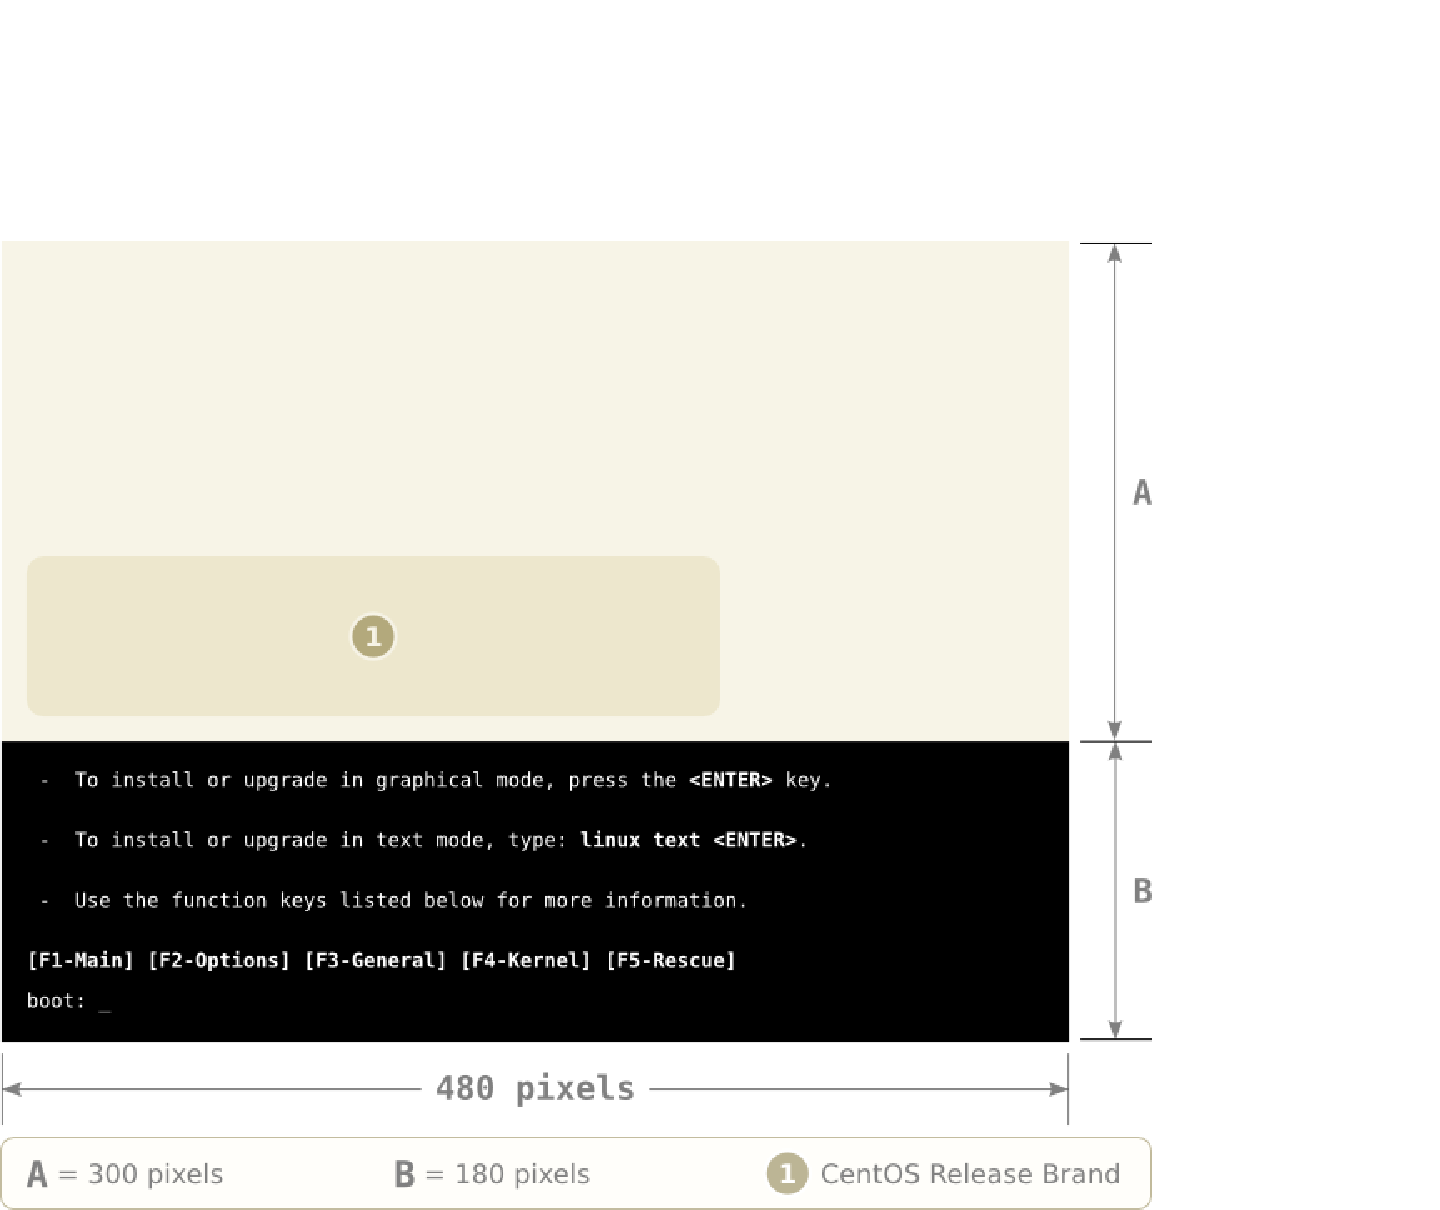
\includegraphics[width=0.8\textwidth]{%
    /home/centos/artwork/trunk/Identity/Models/Img/en/Distro/Anaconda/Prompt/syslinux-splash.pdf}
\end{center}
\caption{Anaconda prompt design model.% 
   \label{fig:Distribution:Anaconda:Model}}
\end{figure}

\begin{figure}[!hbp]
\begin{center}
\fbox{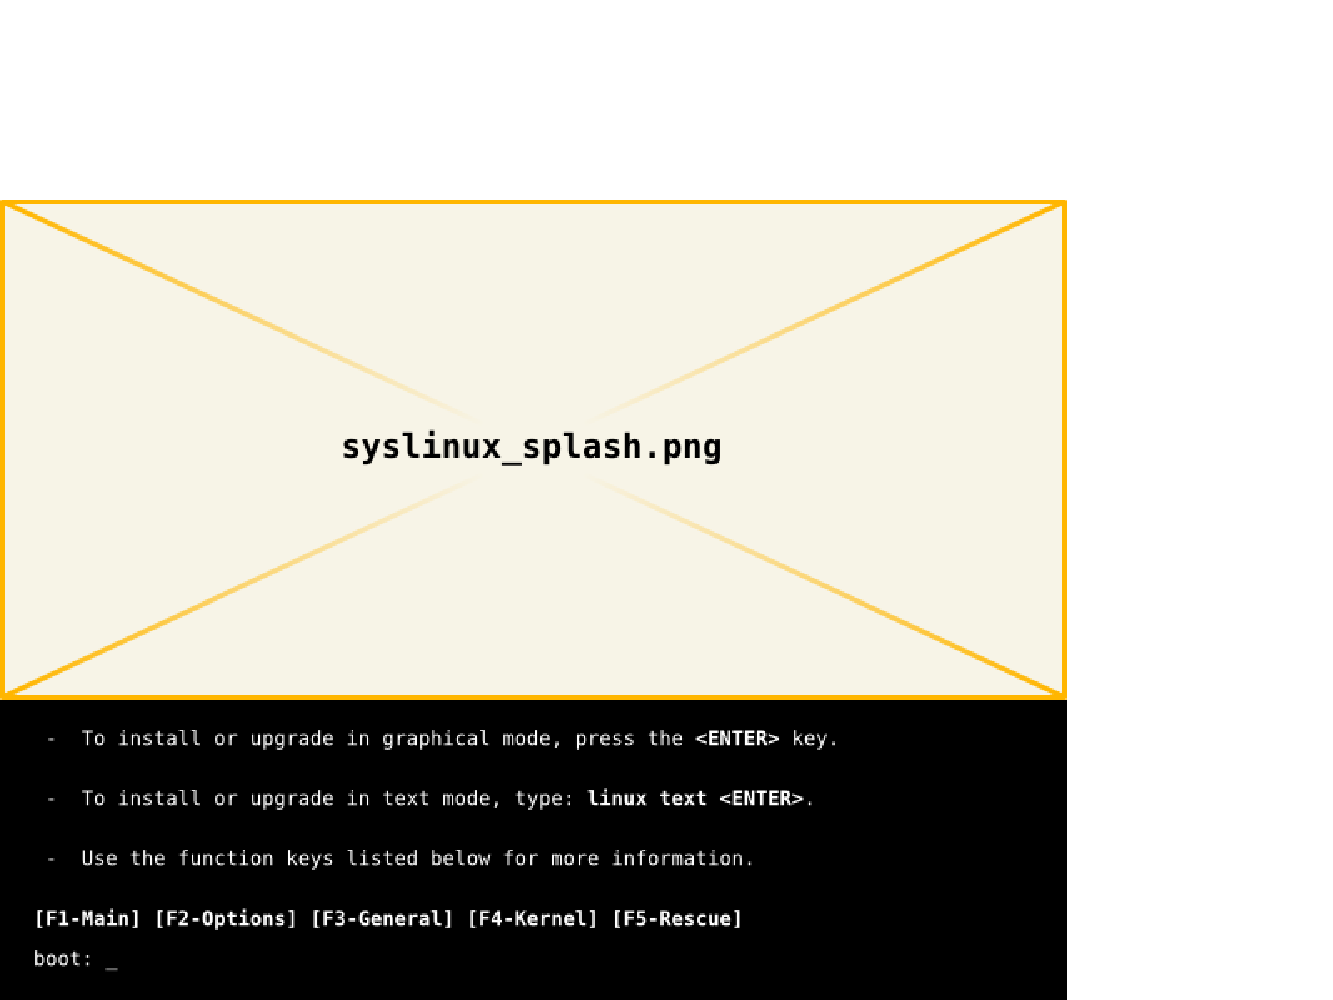
\includegraphics[width=0.8\textwidth]{%
   /home/centos/artwork/trunk/Identity/Models/Img/en/Distro/Anaconda/Prompt/fig-1-syslinux-splash.pdf}} 
\end{center}
\caption{Anaconda prompt position in the screen.% 
   \label{fig:Distribution:Anaconda:Prompt:Models:Fig2}}
\end{figure}

\subsection{Image Files}
\hypertarget{sec:Distribution:Anaconda:Prompt:Identity:Images}{}
\label{sec:Distribution:Anaconda:Prompt:Identity:Images}

\begin{itemize}
\item \texttt{syslinux-splash.png}: base image format.
\item \texttt{syslinux-splash.ppm}: auxiliar format.
\item \texttt{syslinux-splash.pnm}: auxiliar format.
\item \texttt{syslinux-splash.lss}: image format used by syslinux.
\item \texttt{syslinux-splash-16c.pnm}: 16 colors auxiliar format.
\item \texttt{syslinux-splash-16c.png}: 16 colors auxiliar format.
\item \texttt{syslinux-splash.log}: describes image convertion steps.
\end{itemize}

\subsection{Image Files Rendering}
\hypertarget{sec:Distribution:Anaconda:Prompt:Identity:Issues}{}
\label{sec:Distribution:Anaconda:Prompt:Identity:Issues}
\fbox{\texttt{./render.sh}}
\fbox{\texttt{./render.sh '5'}}
\fbox{\texttt{./render.sh '(3|4|5)'}}

\subsection{Color Limitations}
\hypertarget{sec:Distribution:Anaconda:Prompt:Identity:Colors}{}
\label{sec:Distribution:Anaconda:Prompt:Identity:Colors}

Anaconda Prompt does have color limitations. Initially, Anaconda
Prompt images are rendered without color limitation and later they are
indexed to 16 colors and converted to LSS16 format, as described in
\autoref{sec:Concepts:Identity:Themes:Palettes}. 

\subsection{Issues}
\hypertarget{sec:Distribution:Anaconda:Prompt:Issues}{}
\label{sec:Distribution:Anaconda:Prompt:Issues}

When creating Anaconda Prompt images some issues were found. They are
described below:

\begin{itemize}

\item \textbf{Many Different Colors:}

As more different colors you have on your design, more are the
possibilities of increasing the amount of noise in your design after
indexing to 16 colors. For example, if you include the actual CentOS
symbol in this image, it ocupies 3 colors (for the orange, green,
violet) in the indexed image which are completely different and
non-reusable in the blue toned background image.

\item \textbf{The CentOS Symbol:}

As previously said, if we include the CentOS default symbol in
Anaconda Prompt there is a color degradation and a reduction of
available colors to use in the 16 colors indexed image.

Some tests were made with variants of CentOS default symbol, but they
all were declined because they bring confusion about which is the
CentOS default symbol.

It would be very convenient to CentOS visual identity if the CentOS
default symbol could be included, \textit{exactly as it is}, in
Anaconda Prompt images.

\end{itemize}



\section{Translations}
\hypertarget{sec:Distribution:Anaconda:Splash:Translations}{}
\label{sec:Distribution:Anaconda:Splash:Translations}
% ------------------------------------------------------------
% $Id$
% ------------------------------------------------------------
\begin{figure}
\hrulefill
\begin{verbatim}
trunk/Translations/Identity/Themes/Distro/Anaconda/Header/
|-- 3
|   `-- anaconda_header.sed
|-- 4
|-- 5
|-- ... more major releases
|-- render.sh
`-- tpl
    `-- anaconda_header.sed
\end{verbatim}
\hrulefill
\caption{Anaconda header translation framework.%
   \label{fig:Distribution:Anaconda:Header:Translations}}
\end{figure}

% ------------------------------------------------------------ 
\subsection{Translation Markers}
\hypertarget{sec:Distribution:Anaconda:Header:Translations:Markers}{}
\label{sec:Distribution:Anaconda:Header:Translations:Markers}

\begin{itemize}
\item \texttt{=VERSION=}: Major release number of CentOS distribution.
\end{itemize}



\section{Manuals}
\hypertarget{sec:Distribution:Anaconda:Splash:Manuals}{}
\label{sec:Distribution:Anaconda:Splash:Manuals}
% Part   : Concepts
% Chapter: Manuals
% ------------------------------------------------------------
% $Id: manuals.tex 6191 2010-08-02 02:36:14Z al $
% ------------------------------------------------------------

\begin{description}
\item[framework:] trunk/Manuals/
\end{description}

\noindent This chapter describes the CentOS Artwork Repository User
Guide.  The CentOS Artwork Repository User Guide is the book you are
reading right now. The main goals of this book is helping you to
understand how CentOS Artwork Repository works, and what you can do to
get the best of it.  It is also an excuse for you to join us and help
improving it.

\section{Structure}

Inside CentOS Artwork Repository, documentation is conceived using
\LaTeX's book class. Instead of having the entire document in a single
file, information has been spread in separated files under Manuals
framework structure. The Manuals framework structure is illustrated in
\autoref{fig:Concepts:Manuals:Structure} and described in
``\hyperlink{sec:Concepts:Manuals:Files}{Relevant Files}'' (see
\autoref{sec:Concepts:Manuals:Files}) and
``\hyperlink{sec:Concepts:Manuals:Directories}{Relevant Directories}''
(see \autoref{sec:Concepts:Manuals:Directories}).

\begin{figure}[!hbp]
\hrulefill
\begin{verbatim}
trunk/Manuals/
|-- Concepts
|   |-- CentOS
|   |-- Frameworks
|   |-- Identity
|   `-- ...
|-- Distribution
|   |-- Anaconda
|   |   |-- Firstboot
|   |   |-- Header
|   |   |-- Progress
|   |   `-- ...
|   |-- Backgrounds
|   |-- BootUp
|   |   |-- GDM
|   |   |-- GRUB
|   |   `-- ...
|   `-- Release
|-- Licenses
|-- Translations
|-- Workstation
|-- convenctions.tex
|-- repository.aux
|-- repository.lof
|-- repository.log
|-- repository.lot
|-- repository.out
|-- repository.pdf
|-- repository.tex
`-- repository.toc
\end{verbatim}
\hrulefill
\caption{Manuals framework structure.%
   \label{fig:Concepts:Manuals:Structure}}
\end{figure}

\section{Writing Style}

When writing for CentOS Artwork Repository User Guide, keep in mind
the following quote taken from the online ``BBC News Styleguide'':
---The key to good writing is \textbf{simple thoughts simply
expressed}.  Use short sentences and short words.  Anything which is
confused, complicated, poorly written or capable of being
misunderstood risks losing the listener or viewer, and once you have
done that, you might just as well not have come to work---.

If you need to express complicated ideas, try to split them out in
smaller and simpler ideas as much as possible. If you consider it
appropriate, try to use
``\hyperlink{sec:Concepts:Identity:Models}{Design Models}'' (see
\autoref{sec:Concepts:Identity:Models}) to illustrate your thoughts.

\subsection{Cross References}

When you create \LaTeX's cross references, you need to define targets
and links.  Targets are the specific locations in the document that
links point to.  In \LaTeX, these cross reference targets and links
can be defined in many ways, so we need to standardize the way we use
inside CentOS Artwork Repository User Guide to make it look uniform
and easy to read.

Inside CentOS Artwork Repository User Guide, cross references look
like illustrated in
\autoref{fig:Concepts:Manuals:CrossRef:Presentation}.  Cross reference
targets are defined as illustrated in
\autoref{fig:Concepts:Manuals:CrossRef:Targets}, and links to those
targets are defined as illustrated in
\autoref{fig:Concepts:Manuals:CrossRef:Links}. 

Note that we use both \texttt{hypertarget} and \texttt{label} commands
to define targets, and \texttt{hyperlink} and \texttt{autoref} to
define links.  With \texttt{hyperlink} we create long text links
---usefull when reading in the coputer---, and with \texttt{autoref}
we create numbered links ---usefull when reading in a printed copy---.

\begin{figure}[!hbp]
\hrulefill
\begin{flushleft}
\dots you can find more information in
``\hyperlink{sec:Concepts:Identity:Brands}{Logos}'' (see
\autoref{sec:Concepts:Identity:Brands}), specifically in
\hyperlink{sec:Concepts:Identity:Brands:Logos}{the horizontal version} (see
\autoref{sec:Concepts:Identity:Brands:Logos}).
\end{flushleft}
\hrulefill
\caption{Cross reference link presentation.%
   \label{fig:Concepts:Manuals:CrossRef:Presentation}}
\end{figure}

\begin{figure}[!hbp]
\hrulefill
\begin{verbatim}
\part{Concepts}
...
\chapter{The CentOS Logo}
\hypertarget{sec:Concepts:Logo}{}
\label{sec:Concepts:Logo}
...
\section{Horizontal}
\hypertarget{sec:Concepts:Identity:Brands}{}
\label{sec:Concepts:Identity:Brands}
...
\end{verbatim}
\hrulefill
\caption{\LaTeX's definition for cross reference targets.%
   \label{fig:Concepts:Manuals:CrossRef:Targets}}
\end{figure}

\begin{figure}[!hbp]
\hrulefill
\begin{verbatim}
\dots you can find more information in
``\hyperlink{sec:Concepts:Identity:Brands}{The CentOS Logo}'' 
(see \autoref{sec:Concepts:Identity:Brands}), specifically in
\hyperlink{sec:Concepts:Identity:Brands:Logos}{the horizontal version} 
(see \autoref{sec:Concepts:Identity:Brands:Logos}).
\end{verbatim}
\hrulefill
\caption{\LaTeX's definition for cross reference links.%
   \label{fig:Concepts:Manuals:CrossRef:Links}}
\end{figure}

\subsection{Figures}

Inside CentOS Artwork Repository User Guide, illustrations (i.e.
images, framework structures, source code, commands, etc.) are shown
using \LaTeX's \texttt{figure} environment. An example of
\texttt{figure} environment definition is illustrated in
\autoref{fig:Concepts:Manuals:Figures}.  More information about
\LaTeX's \texttt{figure} environment can be found in \LaTeX's info
manual. To read the \LaTeX's info manual, execute in your terminal the
command: \texttt{info latex}.

\begin{figure}[!hbp]
\hrulefill
\begin{verbatim}
\begin{figure}[!hbp]
\hrulefill
...
\hrulefill
\caption{... .%
   \label{fig:...}}
\end{figure}
\end{verbatim}
\hrulefill
\caption{\LaTeX's definition for \texttt{figure} environment.%
   \label{fig:Concepts:Manuals:Figures}}
\end{figure}

\subsection{Tables}

Inside CentOS Artwork Repository User Guide, tabular information (i.e.
translation markers, etc.) is shown using \LaTeX's \texttt{table}
environment. An example of \texttt{table} environment definition is
illustrated in \autoref{fig:Concepts:Manuals:Tables}.  More
information about \LaTeX's \texttt{table} environment can be found in
\LaTeX's info manual. To read the \LaTeX's info manual, execute in
your terminal the command: \texttt{info latex}.

\begin{figure}[!hbp]
\hrulefill
\begin{verbatim}
\begin{table}[!hbp]
\centering
\begin{tabular}[pos]{cols}
\hline
...
\hline
\end{tabular}
\caption{... .%
   \label{tab:...}}
\end{table}
\end{verbatim}
\hrulefill
\caption{\LaTeX's definition for \texttt{table} environment.%
   \label{fig:Concepts:Manuals:Tables}}
\end{figure}

\section{Relevant Files}
\hypertarget{sec:Concepts:Manuals:Files}{}
\label{sec:Concepts:Manuals:Files}

\subsection{repository.tex}

The \texttt{repository.tex} file is the main book's file. Here is
where you define specific book information like class, title, authors,
etc.  Inside \texttt{repository.tex} you organize chapters and load
their sections.

\subsection{introduction.tex} 

The \texttt{Introduction.tex} file introduces a specific artwork
component: what it does, where and when it appears in, etc.

\subsection{framework.tex} 

The \texttt{rramework.tex} file describes how to interact with a
specific artwork component: where to find the artwork component inside
CentOS Artwork Repository, how to render their images, how to render
their translations, their specific translation markers, etc.

\subsection{rebranding.tex} 

The \texttt{rebranding.tex} file describes how to rebrand a specific
artwork component: where to find the arwork component inside CentOS
Distribution, related packages you need to modify, etc.

\section{Relevant Directories}
\hypertarget{sec:Concepts:Manuals:Directories}{}
\label{sec:Concepts:Manuals:Directories}

\subsection{Concepts}

The \texttt{Concepts} directory organizes chapters related to
``Concepts'' part.  Files in this directory describe concepts used
inside CentOS Artwork Repository.

\subsection{Workstation} 

The \texttt{Workstation} directory organizes chapters related to
``Preparing Your Workstation'' part. Files in this directory describe
actions (i.e. installation and configuration) you need to do before
using CentOS Artwork Repository. 

\subsection{Distribution} 

The \texttt{Distribution} directory organizes chapters releated to
``Distribution'' part. This part gets its attention into the different
artwork components of CentOS Distribution, using a subdirectory
structure to organize them and the files \texttt{introduction.tex},
\texttt{framework.tex}, and \texttt{rebranding.tex} to describe them.

\subsection{Licenses} 

The \texttt{Licenses} directory organizes licenses used in this book.

\section{Revisions}
\hypertarget{sec:Concepts:Manuals:Revisions}{}
\label{sec:Concepts:Manuals:Revisions}

Revisions are a way of organizing changes committed to CentOS Artwork
Repository User Guide. Revisions have the format ``Revision M.N'',
where M is the major revision number, and N is the update revision
number.  Revision update number (N) may increase by one every month to
release that month's changes.  Once the six month cycle is reached,
major revision number (M) is increased by one and update revision
number (N) is reset to 0.

\section{Export to PDF}

To produce the file \texttt{repository.pdf}, you need to get inside
the Manual's framework and execute the command:

\begin{quote}
\texttt{pdflatex repository.tex}
\end{quote}


\section{Scripts}
\hypertarget{sec:Distribution:Anaconda:Splash:Scripts}{}
\label{sec:Distribution:Anaconda:Splash:Scripts}
% Part   : Distribution
% Chapter: Anaconda Header
% Section: Scripts
% ------------------------------------------------------------
% $Id$
% ------------------------------------------------------------
\begin{itemize}
\item trunk/Scripts/Identity/Themes/Distro/Anaconda/Header/
\end{itemize}


\section{Packages}
\hypertarget{sec:Distribution:Anaconda:Splash:Packages}{}
\label{sec:Distribution:Anaconda:Splash:Packages}
% ------------------------------------------------------------
% $Id$
% ------------------------------------------------------------
\begin{itemize}
\item \texttt{redhat-logo}
\begin{itemize}
\item /usr/share/anaconda/pixmaps/splash.png
\end{itemize}
\end{itemize}




\chapter{Anaconda Header}
   \hypertarget{cha:Distribution:Anaconda:Header}{}
   \label{cha:Distribution:Anaconda:Header}
   % ------------------------------------------------------------
% $Id$
% ------------------------------------------------------------

\section{Identity}
\hypertarget{sec:Distribution:Anaconda:Splash:Identity}{}
\label{sec:Distribution:Anaconda:Splash:Identity}
% Part   : Distribution
% Chapter: Anaconda Prompt
% Section: Identity
% ------------------------------------------------------------
% $Id$
% ------------------------------------------------------------

\begin{figure}[!hbp]
\hrulefill
\begin{verbatim}
trunk/Identity/Themes/$THEME/Distro/Anaconda/Prompt/
|-- img
|   |-- 3
|   |   |-- syslinux-splash-16c.png
|   |   |-- syslinux-splash-16c.pnm
|   |   |-- syslinux-splash.log
|   |   |-- syslinux-splash.lss
|   |   |-- syslinux-splash.png
|   |   |-- syslinux-splash.pnm
|   |   `-- syslinux-splash.ppm
|   |-- 4
|   |-- 5
|   `-- ... more major releases
|-- render.sh
`-- tpl
    `-- syslinux-splash.svg
\end{verbatim}
\hrulefill
\caption{Anaconda prompt identity's framework.%
   \label{fig:Distribution:Anaconda:Prompt:Identity}}
\end{figure}

\subsection{Designs Templates}
\hypertarget{sec:Distribution:Anaconda:Prompt:Identity:Templates}{}
\label{sec:Distribution:Anaconda:Prompt:Identity:Templates}

\begin{itemize}
\item trunk/Identity/Themes/\$THEME/Distro/Anaconda/Prompt/tpl
\end{itemize}

\subsection{Design Models}

\begin{itemize}
\item trunk/Identity/Models/Tpl/Distro/Anaconda/Prompt/
\item trunk/Identity/Models/Img/Distro/Anaconda/Prompt/
\end{itemize}

\begin{figure}[!hbp]
\begin{center}
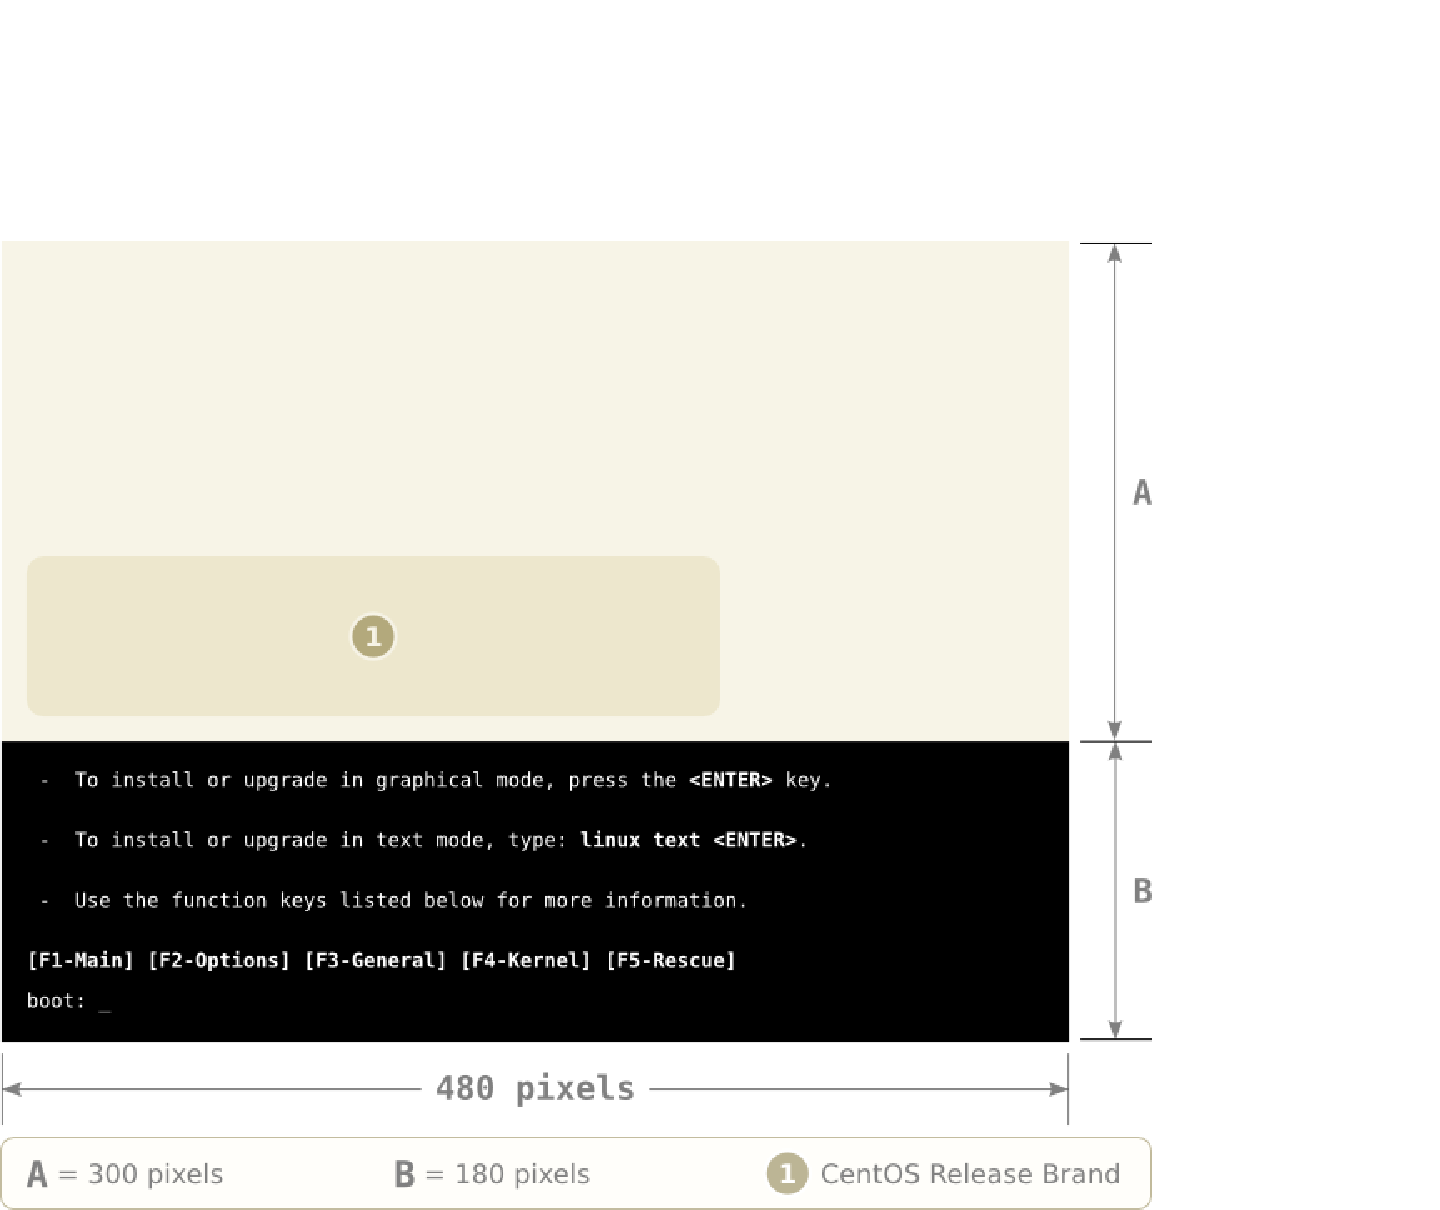
\includegraphics[width=0.8\textwidth]{%
    /home/centos/artwork/trunk/Identity/Models/Img/en/Distro/Anaconda/Prompt/syslinux-splash.pdf}
\end{center}
\caption{Anaconda prompt design model.% 
   \label{fig:Distribution:Anaconda:Model}}
\end{figure}

\begin{figure}[!hbp]
\begin{center}
\fbox{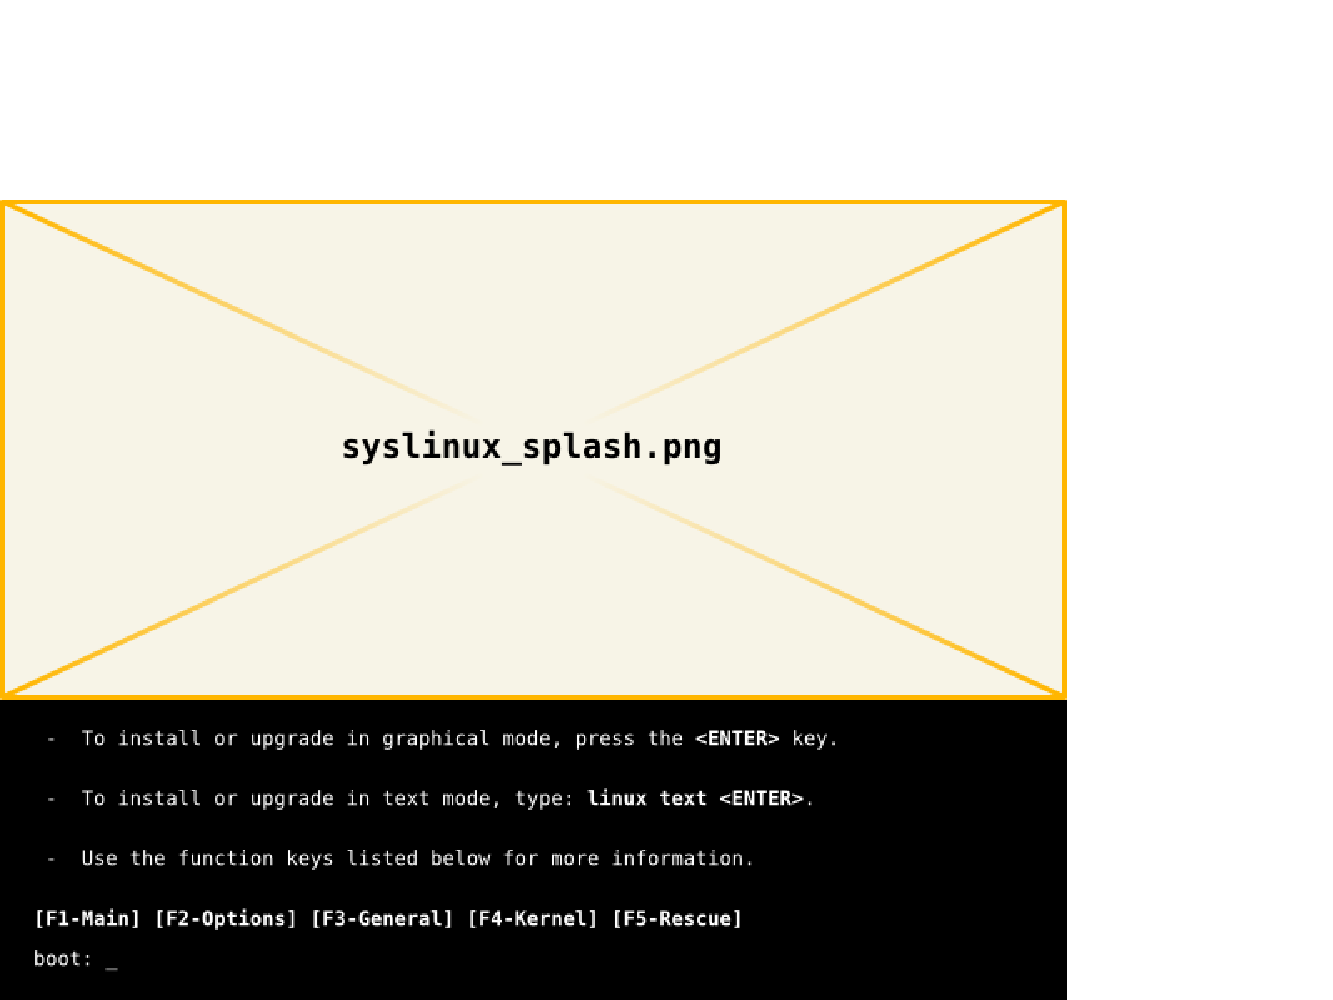
\includegraphics[width=0.8\textwidth]{%
   /home/centos/artwork/trunk/Identity/Models/Img/en/Distro/Anaconda/Prompt/fig-1-syslinux-splash.pdf}} 
\end{center}
\caption{Anaconda prompt position in the screen.% 
   \label{fig:Distribution:Anaconda:Prompt:Models:Fig2}}
\end{figure}

\subsection{Image Files}
\hypertarget{sec:Distribution:Anaconda:Prompt:Identity:Images}{}
\label{sec:Distribution:Anaconda:Prompt:Identity:Images}

\begin{itemize}
\item \texttt{syslinux-splash.png}: base image format.
\item \texttt{syslinux-splash.ppm}: auxiliar format.
\item \texttt{syslinux-splash.pnm}: auxiliar format.
\item \texttt{syslinux-splash.lss}: image format used by syslinux.
\item \texttt{syslinux-splash-16c.pnm}: 16 colors auxiliar format.
\item \texttt{syslinux-splash-16c.png}: 16 colors auxiliar format.
\item \texttt{syslinux-splash.log}: describes image convertion steps.
\end{itemize}

\subsection{Image Files Rendering}
\hypertarget{sec:Distribution:Anaconda:Prompt:Identity:Issues}{}
\label{sec:Distribution:Anaconda:Prompt:Identity:Issues}
\fbox{\texttt{./render.sh}}
\fbox{\texttt{./render.sh '5'}}
\fbox{\texttt{./render.sh '(3|4|5)'}}

\subsection{Color Limitations}
\hypertarget{sec:Distribution:Anaconda:Prompt:Identity:Colors}{}
\label{sec:Distribution:Anaconda:Prompt:Identity:Colors}

Anaconda Prompt does have color limitations. Initially, Anaconda
Prompt images are rendered without color limitation and later they are
indexed to 16 colors and converted to LSS16 format, as described in
\autoref{sec:Concepts:Identity:Themes:Palettes}. 

\subsection{Issues}
\hypertarget{sec:Distribution:Anaconda:Prompt:Issues}{}
\label{sec:Distribution:Anaconda:Prompt:Issues}

When creating Anaconda Prompt images some issues were found. They are
described below:

\begin{itemize}

\item \textbf{Many Different Colors:}

As more different colors you have on your design, more are the
possibilities of increasing the amount of noise in your design after
indexing to 16 colors. For example, if you include the actual CentOS
symbol in this image, it ocupies 3 colors (for the orange, green,
violet) in the indexed image which are completely different and
non-reusable in the blue toned background image.

\item \textbf{The CentOS Symbol:}

As previously said, if we include the CentOS default symbol in
Anaconda Prompt there is a color degradation and a reduction of
available colors to use in the 16 colors indexed image.

Some tests were made with variants of CentOS default symbol, but they
all were declined because they bring confusion about which is the
CentOS default symbol.

It would be very convenient to CentOS visual identity if the CentOS
default symbol could be included, \textit{exactly as it is}, in
Anaconda Prompt images.

\end{itemize}



\section{Translations}
\hypertarget{sec:Distribution:Anaconda:Splash:Translations}{}
\label{sec:Distribution:Anaconda:Splash:Translations}
% ------------------------------------------------------------
% $Id$
% ------------------------------------------------------------
\begin{figure}
\hrulefill
\begin{verbatim}
trunk/Translations/Identity/Themes/Distro/Anaconda/Header/
|-- 3
|   `-- anaconda_header.sed
|-- 4
|-- 5
|-- ... more major releases
|-- render.sh
`-- tpl
    `-- anaconda_header.sed
\end{verbatim}
\hrulefill
\caption{Anaconda header translation framework.%
   \label{fig:Distribution:Anaconda:Header:Translations}}
\end{figure}

% ------------------------------------------------------------ 
\subsection{Translation Markers}
\hypertarget{sec:Distribution:Anaconda:Header:Translations:Markers}{}
\label{sec:Distribution:Anaconda:Header:Translations:Markers}

\begin{itemize}
\item \texttt{=VERSION=}: Major release number of CentOS distribution.
\end{itemize}



\section{Manuals}
\hypertarget{sec:Distribution:Anaconda:Splash:Manuals}{}
\label{sec:Distribution:Anaconda:Splash:Manuals}
% Part   : Concepts
% Chapter: Manuals
% ------------------------------------------------------------
% $Id: manuals.tex 6191 2010-08-02 02:36:14Z al $
% ------------------------------------------------------------

\begin{description}
\item[framework:] trunk/Manuals/
\end{description}

\noindent This chapter describes the CentOS Artwork Repository User
Guide.  The CentOS Artwork Repository User Guide is the book you are
reading right now. The main goals of this book is helping you to
understand how CentOS Artwork Repository works, and what you can do to
get the best of it.  It is also an excuse for you to join us and help
improving it.

\section{Structure}

Inside CentOS Artwork Repository, documentation is conceived using
\LaTeX's book class. Instead of having the entire document in a single
file, information has been spread in separated files under Manuals
framework structure. The Manuals framework structure is illustrated in
\autoref{fig:Concepts:Manuals:Structure} and described in
``\hyperlink{sec:Concepts:Manuals:Files}{Relevant Files}'' (see
\autoref{sec:Concepts:Manuals:Files}) and
``\hyperlink{sec:Concepts:Manuals:Directories}{Relevant Directories}''
(see \autoref{sec:Concepts:Manuals:Directories}).

\begin{figure}[!hbp]
\hrulefill
\begin{verbatim}
trunk/Manuals/
|-- Concepts
|   |-- CentOS
|   |-- Frameworks
|   |-- Identity
|   `-- ...
|-- Distribution
|   |-- Anaconda
|   |   |-- Firstboot
|   |   |-- Header
|   |   |-- Progress
|   |   `-- ...
|   |-- Backgrounds
|   |-- BootUp
|   |   |-- GDM
|   |   |-- GRUB
|   |   `-- ...
|   `-- Release
|-- Licenses
|-- Translations
|-- Workstation
|-- convenctions.tex
|-- repository.aux
|-- repository.lof
|-- repository.log
|-- repository.lot
|-- repository.out
|-- repository.pdf
|-- repository.tex
`-- repository.toc
\end{verbatim}
\hrulefill
\caption{Manuals framework structure.%
   \label{fig:Concepts:Manuals:Structure}}
\end{figure}

\section{Writing Style}

When writing for CentOS Artwork Repository User Guide, keep in mind
the following quote taken from the online ``BBC News Styleguide'':
---The key to good writing is \textbf{simple thoughts simply
expressed}.  Use short sentences and short words.  Anything which is
confused, complicated, poorly written or capable of being
misunderstood risks losing the listener or viewer, and once you have
done that, you might just as well not have come to work---.

If you need to express complicated ideas, try to split them out in
smaller and simpler ideas as much as possible. If you consider it
appropriate, try to use
``\hyperlink{sec:Concepts:Identity:Models}{Design Models}'' (see
\autoref{sec:Concepts:Identity:Models}) to illustrate your thoughts.

\subsection{Cross References}

When you create \LaTeX's cross references, you need to define targets
and links.  Targets are the specific locations in the document that
links point to.  In \LaTeX, these cross reference targets and links
can be defined in many ways, so we need to standardize the way we use
inside CentOS Artwork Repository User Guide to make it look uniform
and easy to read.

Inside CentOS Artwork Repository User Guide, cross references look
like illustrated in
\autoref{fig:Concepts:Manuals:CrossRef:Presentation}.  Cross reference
targets are defined as illustrated in
\autoref{fig:Concepts:Manuals:CrossRef:Targets}, and links to those
targets are defined as illustrated in
\autoref{fig:Concepts:Manuals:CrossRef:Links}. 

Note that we use both \texttt{hypertarget} and \texttt{label} commands
to define targets, and \texttt{hyperlink} and \texttt{autoref} to
define links.  With \texttt{hyperlink} we create long text links
---usefull when reading in the coputer---, and with \texttt{autoref}
we create numbered links ---usefull when reading in a printed copy---.

\begin{figure}[!hbp]
\hrulefill
\begin{flushleft}
\dots you can find more information in
``\hyperlink{sec:Concepts:Identity:Brands}{Logos}'' (see
\autoref{sec:Concepts:Identity:Brands}), specifically in
\hyperlink{sec:Concepts:Identity:Brands:Logos}{the horizontal version} (see
\autoref{sec:Concepts:Identity:Brands:Logos}).
\end{flushleft}
\hrulefill
\caption{Cross reference link presentation.%
   \label{fig:Concepts:Manuals:CrossRef:Presentation}}
\end{figure}

\begin{figure}[!hbp]
\hrulefill
\begin{verbatim}
\part{Concepts}
...
\chapter{The CentOS Logo}
\hypertarget{sec:Concepts:Logo}{}
\label{sec:Concepts:Logo}
...
\section{Horizontal}
\hypertarget{sec:Concepts:Identity:Brands}{}
\label{sec:Concepts:Identity:Brands}
...
\end{verbatim}
\hrulefill
\caption{\LaTeX's definition for cross reference targets.%
   \label{fig:Concepts:Manuals:CrossRef:Targets}}
\end{figure}

\begin{figure}[!hbp]
\hrulefill
\begin{verbatim}
\dots you can find more information in
``\hyperlink{sec:Concepts:Identity:Brands}{The CentOS Logo}'' 
(see \autoref{sec:Concepts:Identity:Brands}), specifically in
\hyperlink{sec:Concepts:Identity:Brands:Logos}{the horizontal version} 
(see \autoref{sec:Concepts:Identity:Brands:Logos}).
\end{verbatim}
\hrulefill
\caption{\LaTeX's definition for cross reference links.%
   \label{fig:Concepts:Manuals:CrossRef:Links}}
\end{figure}

\subsection{Figures}

Inside CentOS Artwork Repository User Guide, illustrations (i.e.
images, framework structures, source code, commands, etc.) are shown
using \LaTeX's \texttt{figure} environment. An example of
\texttt{figure} environment definition is illustrated in
\autoref{fig:Concepts:Manuals:Figures}.  More information about
\LaTeX's \texttt{figure} environment can be found in \LaTeX's info
manual. To read the \LaTeX's info manual, execute in your terminal the
command: \texttt{info latex}.

\begin{figure}[!hbp]
\hrulefill
\begin{verbatim}
\begin{figure}[!hbp]
\hrulefill
...
\hrulefill
\caption{... .%
   \label{fig:...}}
\end{figure}
\end{verbatim}
\hrulefill
\caption{\LaTeX's definition for \texttt{figure} environment.%
   \label{fig:Concepts:Manuals:Figures}}
\end{figure}

\subsection{Tables}

Inside CentOS Artwork Repository User Guide, tabular information (i.e.
translation markers, etc.) is shown using \LaTeX's \texttt{table}
environment. An example of \texttt{table} environment definition is
illustrated in \autoref{fig:Concepts:Manuals:Tables}.  More
information about \LaTeX's \texttt{table} environment can be found in
\LaTeX's info manual. To read the \LaTeX's info manual, execute in
your terminal the command: \texttt{info latex}.

\begin{figure}[!hbp]
\hrulefill
\begin{verbatim}
\begin{table}[!hbp]
\centering
\begin{tabular}[pos]{cols}
\hline
...
\hline
\end{tabular}
\caption{... .%
   \label{tab:...}}
\end{table}
\end{verbatim}
\hrulefill
\caption{\LaTeX's definition for \texttt{table} environment.%
   \label{fig:Concepts:Manuals:Tables}}
\end{figure}

\section{Relevant Files}
\hypertarget{sec:Concepts:Manuals:Files}{}
\label{sec:Concepts:Manuals:Files}

\subsection{repository.tex}

The \texttt{repository.tex} file is the main book's file. Here is
where you define specific book information like class, title, authors,
etc.  Inside \texttt{repository.tex} you organize chapters and load
their sections.

\subsection{introduction.tex} 

The \texttt{Introduction.tex} file introduces a specific artwork
component: what it does, where and when it appears in, etc.

\subsection{framework.tex} 

The \texttt{rramework.tex} file describes how to interact with a
specific artwork component: where to find the artwork component inside
CentOS Artwork Repository, how to render their images, how to render
their translations, their specific translation markers, etc.

\subsection{rebranding.tex} 

The \texttt{rebranding.tex} file describes how to rebrand a specific
artwork component: where to find the arwork component inside CentOS
Distribution, related packages you need to modify, etc.

\section{Relevant Directories}
\hypertarget{sec:Concepts:Manuals:Directories}{}
\label{sec:Concepts:Manuals:Directories}

\subsection{Concepts}

The \texttt{Concepts} directory organizes chapters related to
``Concepts'' part.  Files in this directory describe concepts used
inside CentOS Artwork Repository.

\subsection{Workstation} 

The \texttt{Workstation} directory organizes chapters related to
``Preparing Your Workstation'' part. Files in this directory describe
actions (i.e. installation and configuration) you need to do before
using CentOS Artwork Repository. 

\subsection{Distribution} 

The \texttt{Distribution} directory organizes chapters releated to
``Distribution'' part. This part gets its attention into the different
artwork components of CentOS Distribution, using a subdirectory
structure to organize them and the files \texttt{introduction.tex},
\texttt{framework.tex}, and \texttt{rebranding.tex} to describe them.

\subsection{Licenses} 

The \texttt{Licenses} directory organizes licenses used in this book.

\section{Revisions}
\hypertarget{sec:Concepts:Manuals:Revisions}{}
\label{sec:Concepts:Manuals:Revisions}

Revisions are a way of organizing changes committed to CentOS Artwork
Repository User Guide. Revisions have the format ``Revision M.N'',
where M is the major revision number, and N is the update revision
number.  Revision update number (N) may increase by one every month to
release that month's changes.  Once the six month cycle is reached,
major revision number (M) is increased by one and update revision
number (N) is reset to 0.

\section{Export to PDF}

To produce the file \texttt{repository.pdf}, you need to get inside
the Manual's framework and execute the command:

\begin{quote}
\texttt{pdflatex repository.tex}
\end{quote}


\section{Scripts}
\hypertarget{sec:Distribution:Anaconda:Splash:Scripts}{}
\label{sec:Distribution:Anaconda:Splash:Scripts}
% Part   : Distribution
% Chapter: Anaconda Header
% Section: Scripts
% ------------------------------------------------------------
% $Id$
% ------------------------------------------------------------
\begin{itemize}
\item trunk/Scripts/Identity/Themes/Distro/Anaconda/Header/
\end{itemize}


\section{Packages}
\hypertarget{sec:Distribution:Anaconda:Splash:Packages}{}
\label{sec:Distribution:Anaconda:Splash:Packages}
% ------------------------------------------------------------
% $Id$
% ------------------------------------------------------------
\begin{itemize}
\item \texttt{redhat-logo}
\begin{itemize}
\item /usr/share/anaconda/pixmaps/splash.png
\end{itemize}
\end{itemize}




\chapter{Anaconda Splash}
   \hypertarget{cha:Distribution:Anaconda:Splash}{}
   \label{cha:Distribution:Anaconda:Splash}
   % ------------------------------------------------------------
% $Id$
% ------------------------------------------------------------

\section{Identity}
\hypertarget{sec:Distribution:Anaconda:Splash:Identity}{}
\label{sec:Distribution:Anaconda:Splash:Identity}
% Part   : Distribution
% Chapter: Anaconda Prompt
% Section: Identity
% ------------------------------------------------------------
% $Id$
% ------------------------------------------------------------

\begin{figure}[!hbp]
\hrulefill
\begin{verbatim}
trunk/Identity/Themes/$THEME/Distro/Anaconda/Prompt/
|-- img
|   |-- 3
|   |   |-- syslinux-splash-16c.png
|   |   |-- syslinux-splash-16c.pnm
|   |   |-- syslinux-splash.log
|   |   |-- syslinux-splash.lss
|   |   |-- syslinux-splash.png
|   |   |-- syslinux-splash.pnm
|   |   `-- syslinux-splash.ppm
|   |-- 4
|   |-- 5
|   `-- ... more major releases
|-- render.sh
`-- tpl
    `-- syslinux-splash.svg
\end{verbatim}
\hrulefill
\caption{Anaconda prompt identity's framework.%
   \label{fig:Distribution:Anaconda:Prompt:Identity}}
\end{figure}

\subsection{Designs Templates}
\hypertarget{sec:Distribution:Anaconda:Prompt:Identity:Templates}{}
\label{sec:Distribution:Anaconda:Prompt:Identity:Templates}

\begin{itemize}
\item trunk/Identity/Themes/\$THEME/Distro/Anaconda/Prompt/tpl
\end{itemize}

\subsection{Design Models}

\begin{itemize}
\item trunk/Identity/Models/Tpl/Distro/Anaconda/Prompt/
\item trunk/Identity/Models/Img/Distro/Anaconda/Prompt/
\end{itemize}

\begin{figure}[!hbp]
\begin{center}
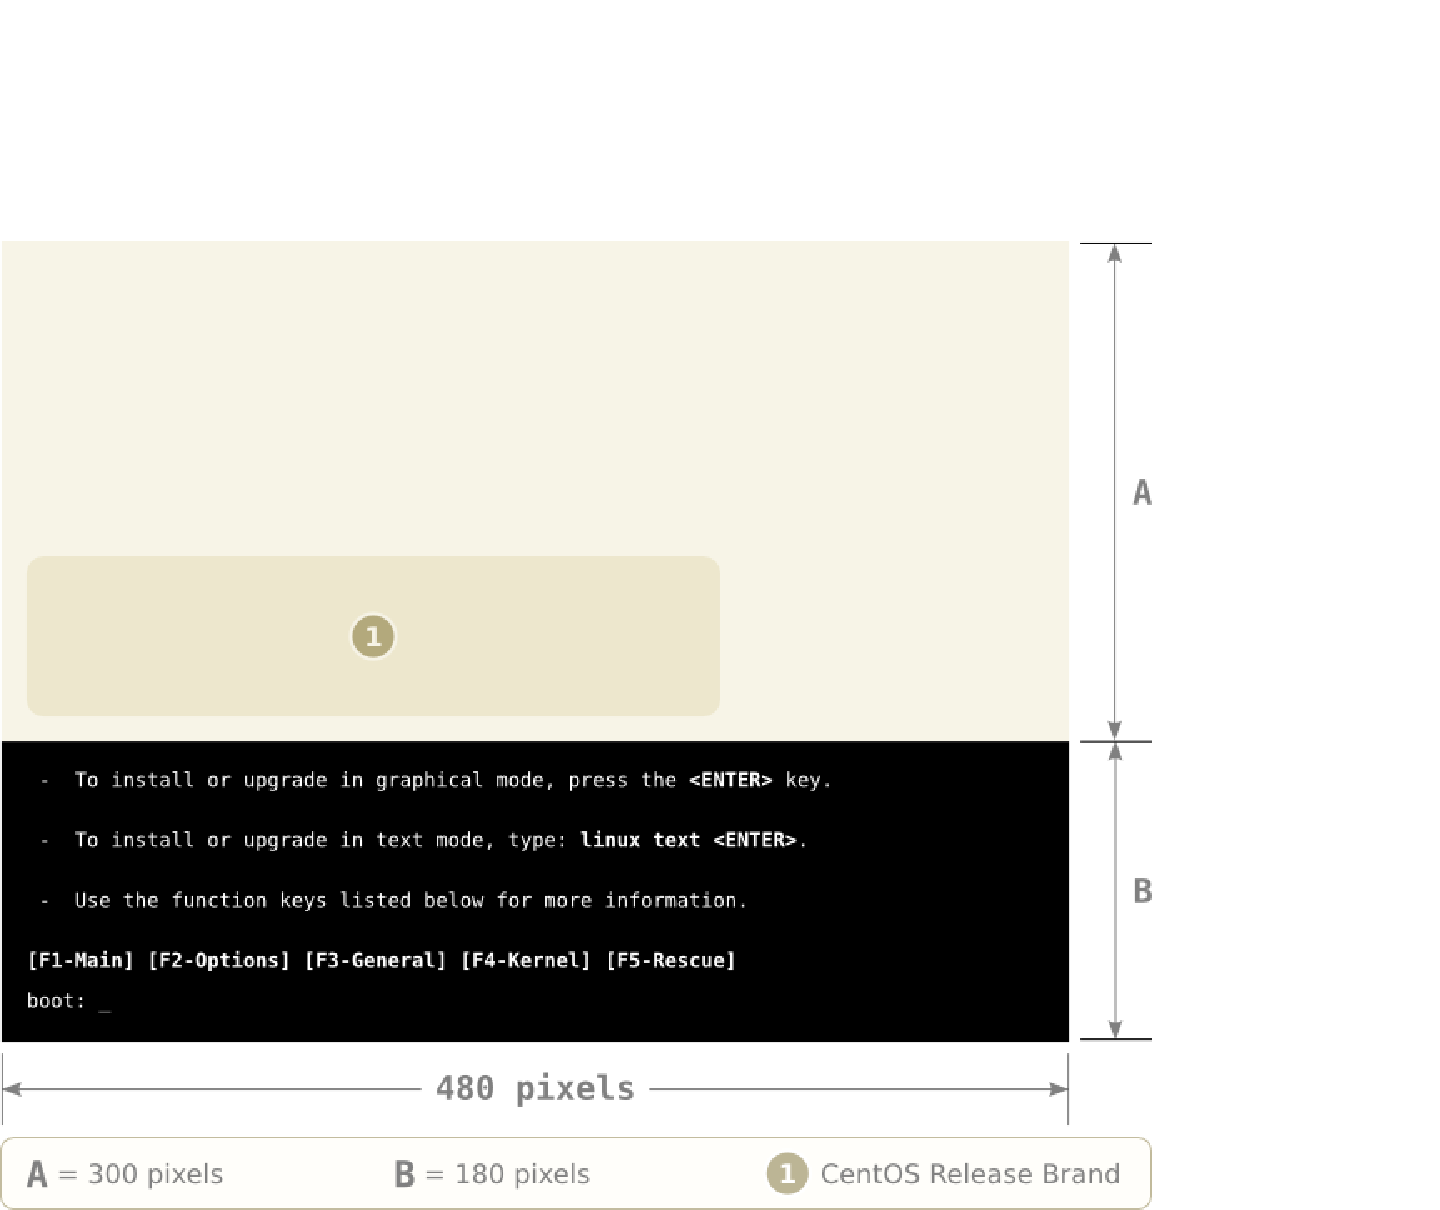
\includegraphics[width=0.8\textwidth]{%
    /home/centos/artwork/trunk/Identity/Models/Img/en/Distro/Anaconda/Prompt/syslinux-splash.pdf}
\end{center}
\caption{Anaconda prompt design model.% 
   \label{fig:Distribution:Anaconda:Model}}
\end{figure}

\begin{figure}[!hbp]
\begin{center}
\fbox{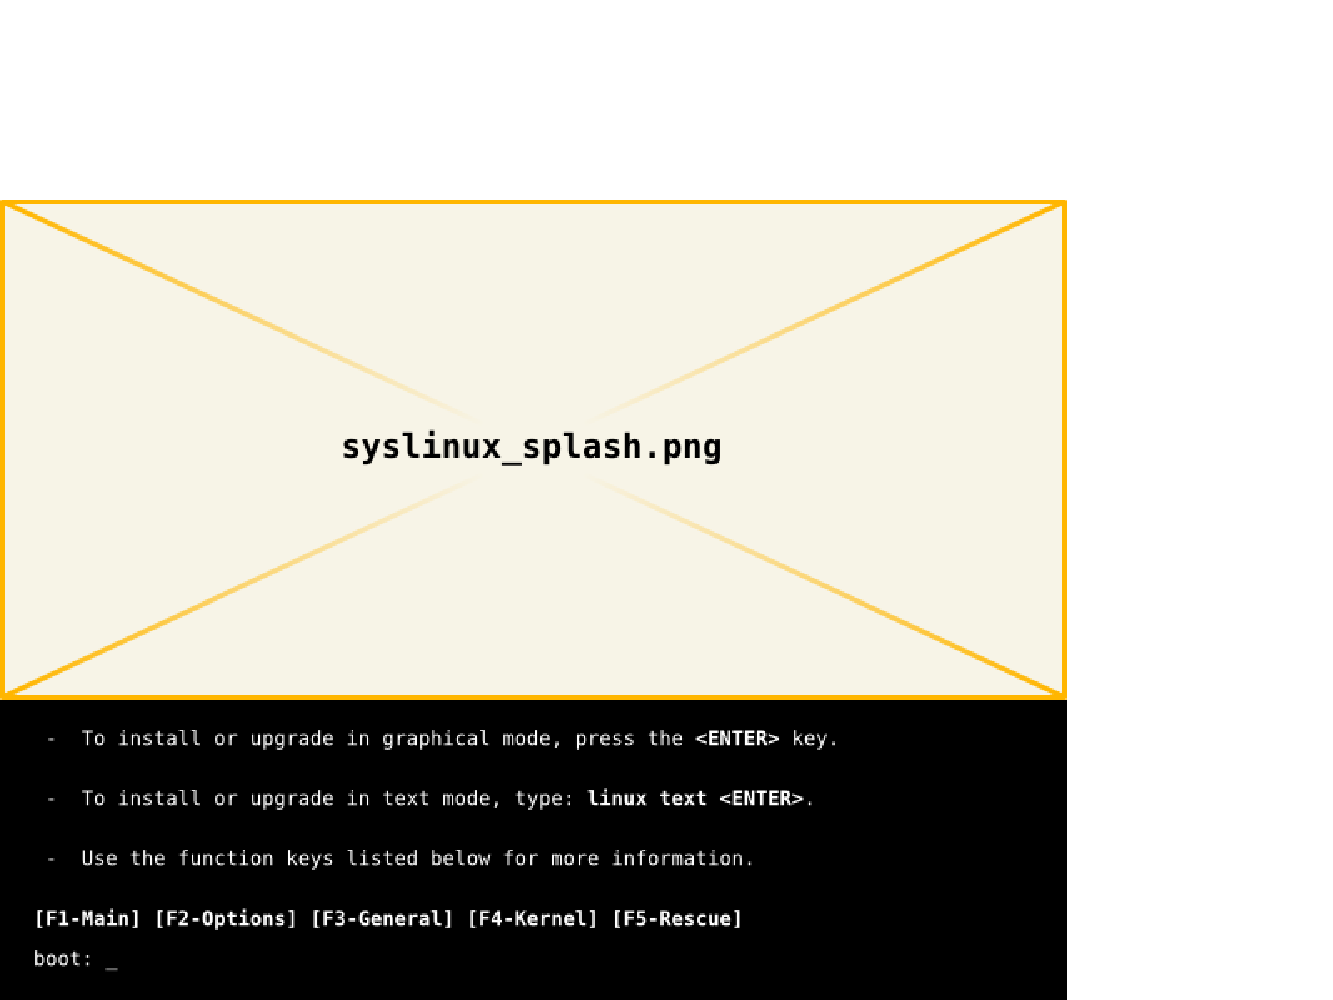
\includegraphics[width=0.8\textwidth]{%
   /home/centos/artwork/trunk/Identity/Models/Img/en/Distro/Anaconda/Prompt/fig-1-syslinux-splash.pdf}} 
\end{center}
\caption{Anaconda prompt position in the screen.% 
   \label{fig:Distribution:Anaconda:Prompt:Models:Fig2}}
\end{figure}

\subsection{Image Files}
\hypertarget{sec:Distribution:Anaconda:Prompt:Identity:Images}{}
\label{sec:Distribution:Anaconda:Prompt:Identity:Images}

\begin{itemize}
\item \texttt{syslinux-splash.png}: base image format.
\item \texttt{syslinux-splash.ppm}: auxiliar format.
\item \texttt{syslinux-splash.pnm}: auxiliar format.
\item \texttt{syslinux-splash.lss}: image format used by syslinux.
\item \texttt{syslinux-splash-16c.pnm}: 16 colors auxiliar format.
\item \texttt{syslinux-splash-16c.png}: 16 colors auxiliar format.
\item \texttt{syslinux-splash.log}: describes image convertion steps.
\end{itemize}

\subsection{Image Files Rendering}
\hypertarget{sec:Distribution:Anaconda:Prompt:Identity:Issues}{}
\label{sec:Distribution:Anaconda:Prompt:Identity:Issues}
\fbox{\texttt{./render.sh}}
\fbox{\texttt{./render.sh '5'}}
\fbox{\texttt{./render.sh '(3|4|5)'}}

\subsection{Color Limitations}
\hypertarget{sec:Distribution:Anaconda:Prompt:Identity:Colors}{}
\label{sec:Distribution:Anaconda:Prompt:Identity:Colors}

Anaconda Prompt does have color limitations. Initially, Anaconda
Prompt images are rendered without color limitation and later they are
indexed to 16 colors and converted to LSS16 format, as described in
\autoref{sec:Concepts:Identity:Themes:Palettes}. 

\subsection{Issues}
\hypertarget{sec:Distribution:Anaconda:Prompt:Issues}{}
\label{sec:Distribution:Anaconda:Prompt:Issues}

When creating Anaconda Prompt images some issues were found. They are
described below:

\begin{itemize}

\item \textbf{Many Different Colors:}

As more different colors you have on your design, more are the
possibilities of increasing the amount of noise in your design after
indexing to 16 colors. For example, if you include the actual CentOS
symbol in this image, it ocupies 3 colors (for the orange, green,
violet) in the indexed image which are completely different and
non-reusable in the blue toned background image.

\item \textbf{The CentOS Symbol:}

As previously said, if we include the CentOS default symbol in
Anaconda Prompt there is a color degradation and a reduction of
available colors to use in the 16 colors indexed image.

Some tests were made with variants of CentOS default symbol, but they
all were declined because they bring confusion about which is the
CentOS default symbol.

It would be very convenient to CentOS visual identity if the CentOS
default symbol could be included, \textit{exactly as it is}, in
Anaconda Prompt images.

\end{itemize}



\section{Translations}
\hypertarget{sec:Distribution:Anaconda:Splash:Translations}{}
\label{sec:Distribution:Anaconda:Splash:Translations}
% ------------------------------------------------------------
% $Id$
% ------------------------------------------------------------
\begin{figure}
\hrulefill
\begin{verbatim}
trunk/Translations/Identity/Themes/Distro/Anaconda/Header/
|-- 3
|   `-- anaconda_header.sed
|-- 4
|-- 5
|-- ... more major releases
|-- render.sh
`-- tpl
    `-- anaconda_header.sed
\end{verbatim}
\hrulefill
\caption{Anaconda header translation framework.%
   \label{fig:Distribution:Anaconda:Header:Translations}}
\end{figure}

% ------------------------------------------------------------ 
\subsection{Translation Markers}
\hypertarget{sec:Distribution:Anaconda:Header:Translations:Markers}{}
\label{sec:Distribution:Anaconda:Header:Translations:Markers}

\begin{itemize}
\item \texttt{=VERSION=}: Major release number of CentOS distribution.
\end{itemize}



\section{Manuals}
\hypertarget{sec:Distribution:Anaconda:Splash:Manuals}{}
\label{sec:Distribution:Anaconda:Splash:Manuals}
% Part   : Concepts
% Chapter: Manuals
% ------------------------------------------------------------
% $Id: manuals.tex 6191 2010-08-02 02:36:14Z al $
% ------------------------------------------------------------

\begin{description}
\item[framework:] trunk/Manuals/
\end{description}

\noindent This chapter describes the CentOS Artwork Repository User
Guide.  The CentOS Artwork Repository User Guide is the book you are
reading right now. The main goals of this book is helping you to
understand how CentOS Artwork Repository works, and what you can do to
get the best of it.  It is also an excuse for you to join us and help
improving it.

\section{Structure}

Inside CentOS Artwork Repository, documentation is conceived using
\LaTeX's book class. Instead of having the entire document in a single
file, information has been spread in separated files under Manuals
framework structure. The Manuals framework structure is illustrated in
\autoref{fig:Concepts:Manuals:Structure} and described in
``\hyperlink{sec:Concepts:Manuals:Files}{Relevant Files}'' (see
\autoref{sec:Concepts:Manuals:Files}) and
``\hyperlink{sec:Concepts:Manuals:Directories}{Relevant Directories}''
(see \autoref{sec:Concepts:Manuals:Directories}).

\begin{figure}[!hbp]
\hrulefill
\begin{verbatim}
trunk/Manuals/
|-- Concepts
|   |-- CentOS
|   |-- Frameworks
|   |-- Identity
|   `-- ...
|-- Distribution
|   |-- Anaconda
|   |   |-- Firstboot
|   |   |-- Header
|   |   |-- Progress
|   |   `-- ...
|   |-- Backgrounds
|   |-- BootUp
|   |   |-- GDM
|   |   |-- GRUB
|   |   `-- ...
|   `-- Release
|-- Licenses
|-- Translations
|-- Workstation
|-- convenctions.tex
|-- repository.aux
|-- repository.lof
|-- repository.log
|-- repository.lot
|-- repository.out
|-- repository.pdf
|-- repository.tex
`-- repository.toc
\end{verbatim}
\hrulefill
\caption{Manuals framework structure.%
   \label{fig:Concepts:Manuals:Structure}}
\end{figure}

\section{Writing Style}

When writing for CentOS Artwork Repository User Guide, keep in mind
the following quote taken from the online ``BBC News Styleguide'':
---The key to good writing is \textbf{simple thoughts simply
expressed}.  Use short sentences and short words.  Anything which is
confused, complicated, poorly written or capable of being
misunderstood risks losing the listener or viewer, and once you have
done that, you might just as well not have come to work---.

If you need to express complicated ideas, try to split them out in
smaller and simpler ideas as much as possible. If you consider it
appropriate, try to use
``\hyperlink{sec:Concepts:Identity:Models}{Design Models}'' (see
\autoref{sec:Concepts:Identity:Models}) to illustrate your thoughts.

\subsection{Cross References}

When you create \LaTeX's cross references, you need to define targets
and links.  Targets are the specific locations in the document that
links point to.  In \LaTeX, these cross reference targets and links
can be defined in many ways, so we need to standardize the way we use
inside CentOS Artwork Repository User Guide to make it look uniform
and easy to read.

Inside CentOS Artwork Repository User Guide, cross references look
like illustrated in
\autoref{fig:Concepts:Manuals:CrossRef:Presentation}.  Cross reference
targets are defined as illustrated in
\autoref{fig:Concepts:Manuals:CrossRef:Targets}, and links to those
targets are defined as illustrated in
\autoref{fig:Concepts:Manuals:CrossRef:Links}. 

Note that we use both \texttt{hypertarget} and \texttt{label} commands
to define targets, and \texttt{hyperlink} and \texttt{autoref} to
define links.  With \texttt{hyperlink} we create long text links
---usefull when reading in the coputer---, and with \texttt{autoref}
we create numbered links ---usefull when reading in a printed copy---.

\begin{figure}[!hbp]
\hrulefill
\begin{flushleft}
\dots you can find more information in
``\hyperlink{sec:Concepts:Identity:Brands}{Logos}'' (see
\autoref{sec:Concepts:Identity:Brands}), specifically in
\hyperlink{sec:Concepts:Identity:Brands:Logos}{the horizontal version} (see
\autoref{sec:Concepts:Identity:Brands:Logos}).
\end{flushleft}
\hrulefill
\caption{Cross reference link presentation.%
   \label{fig:Concepts:Manuals:CrossRef:Presentation}}
\end{figure}

\begin{figure}[!hbp]
\hrulefill
\begin{verbatim}
\part{Concepts}
...
\chapter{The CentOS Logo}
\hypertarget{sec:Concepts:Logo}{}
\label{sec:Concepts:Logo}
...
\section{Horizontal}
\hypertarget{sec:Concepts:Identity:Brands}{}
\label{sec:Concepts:Identity:Brands}
...
\end{verbatim}
\hrulefill
\caption{\LaTeX's definition for cross reference targets.%
   \label{fig:Concepts:Manuals:CrossRef:Targets}}
\end{figure}

\begin{figure}[!hbp]
\hrulefill
\begin{verbatim}
\dots you can find more information in
``\hyperlink{sec:Concepts:Identity:Brands}{The CentOS Logo}'' 
(see \autoref{sec:Concepts:Identity:Brands}), specifically in
\hyperlink{sec:Concepts:Identity:Brands:Logos}{the horizontal version} 
(see \autoref{sec:Concepts:Identity:Brands:Logos}).
\end{verbatim}
\hrulefill
\caption{\LaTeX's definition for cross reference links.%
   \label{fig:Concepts:Manuals:CrossRef:Links}}
\end{figure}

\subsection{Figures}

Inside CentOS Artwork Repository User Guide, illustrations (i.e.
images, framework structures, source code, commands, etc.) are shown
using \LaTeX's \texttt{figure} environment. An example of
\texttt{figure} environment definition is illustrated in
\autoref{fig:Concepts:Manuals:Figures}.  More information about
\LaTeX's \texttt{figure} environment can be found in \LaTeX's info
manual. To read the \LaTeX's info manual, execute in your terminal the
command: \texttt{info latex}.

\begin{figure}[!hbp]
\hrulefill
\begin{verbatim}
\begin{figure}[!hbp]
\hrulefill
...
\hrulefill
\caption{... .%
   \label{fig:...}}
\end{figure}
\end{verbatim}
\hrulefill
\caption{\LaTeX's definition for \texttt{figure} environment.%
   \label{fig:Concepts:Manuals:Figures}}
\end{figure}

\subsection{Tables}

Inside CentOS Artwork Repository User Guide, tabular information (i.e.
translation markers, etc.) is shown using \LaTeX's \texttt{table}
environment. An example of \texttt{table} environment definition is
illustrated in \autoref{fig:Concepts:Manuals:Tables}.  More
information about \LaTeX's \texttt{table} environment can be found in
\LaTeX's info manual. To read the \LaTeX's info manual, execute in
your terminal the command: \texttt{info latex}.

\begin{figure}[!hbp]
\hrulefill
\begin{verbatim}
\begin{table}[!hbp]
\centering
\begin{tabular}[pos]{cols}
\hline
...
\hline
\end{tabular}
\caption{... .%
   \label{tab:...}}
\end{table}
\end{verbatim}
\hrulefill
\caption{\LaTeX's definition for \texttt{table} environment.%
   \label{fig:Concepts:Manuals:Tables}}
\end{figure}

\section{Relevant Files}
\hypertarget{sec:Concepts:Manuals:Files}{}
\label{sec:Concepts:Manuals:Files}

\subsection{repository.tex}

The \texttt{repository.tex} file is the main book's file. Here is
where you define specific book information like class, title, authors,
etc.  Inside \texttt{repository.tex} you organize chapters and load
their sections.

\subsection{introduction.tex} 

The \texttt{Introduction.tex} file introduces a specific artwork
component: what it does, where and when it appears in, etc.

\subsection{framework.tex} 

The \texttt{rramework.tex} file describes how to interact with a
specific artwork component: where to find the artwork component inside
CentOS Artwork Repository, how to render their images, how to render
their translations, their specific translation markers, etc.

\subsection{rebranding.tex} 

The \texttt{rebranding.tex} file describes how to rebrand a specific
artwork component: where to find the arwork component inside CentOS
Distribution, related packages you need to modify, etc.

\section{Relevant Directories}
\hypertarget{sec:Concepts:Manuals:Directories}{}
\label{sec:Concepts:Manuals:Directories}

\subsection{Concepts}

The \texttt{Concepts} directory organizes chapters related to
``Concepts'' part.  Files in this directory describe concepts used
inside CentOS Artwork Repository.

\subsection{Workstation} 

The \texttt{Workstation} directory organizes chapters related to
``Preparing Your Workstation'' part. Files in this directory describe
actions (i.e. installation and configuration) you need to do before
using CentOS Artwork Repository. 

\subsection{Distribution} 

The \texttt{Distribution} directory organizes chapters releated to
``Distribution'' part. This part gets its attention into the different
artwork components of CentOS Distribution, using a subdirectory
structure to organize them and the files \texttt{introduction.tex},
\texttt{framework.tex}, and \texttt{rebranding.tex} to describe them.

\subsection{Licenses} 

The \texttt{Licenses} directory organizes licenses used in this book.

\section{Revisions}
\hypertarget{sec:Concepts:Manuals:Revisions}{}
\label{sec:Concepts:Manuals:Revisions}

Revisions are a way of organizing changes committed to CentOS Artwork
Repository User Guide. Revisions have the format ``Revision M.N'',
where M is the major revision number, and N is the update revision
number.  Revision update number (N) may increase by one every month to
release that month's changes.  Once the six month cycle is reached,
major revision number (M) is increased by one and update revision
number (N) is reset to 0.

\section{Export to PDF}

To produce the file \texttt{repository.pdf}, you need to get inside
the Manual's framework and execute the command:

\begin{quote}
\texttt{pdflatex repository.tex}
\end{quote}


\section{Scripts}
\hypertarget{sec:Distribution:Anaconda:Splash:Scripts}{}
\label{sec:Distribution:Anaconda:Splash:Scripts}
% Part   : Distribution
% Chapter: Anaconda Header
% Section: Scripts
% ------------------------------------------------------------
% $Id$
% ------------------------------------------------------------
\begin{itemize}
\item trunk/Scripts/Identity/Themes/Distro/Anaconda/Header/
\end{itemize}


\section{Packages}
\hypertarget{sec:Distribution:Anaconda:Splash:Packages}{}
\label{sec:Distribution:Anaconda:Splash:Packages}
% ------------------------------------------------------------
% $Id$
% ------------------------------------------------------------
\begin{itemize}
\item \texttt{redhat-logo}
\begin{itemize}
\item /usr/share/anaconda/pixmaps/splash.png
\end{itemize}
\end{itemize}




\chapter{Anaconda Progress}
   \hypertarget{cha:Distribution:Anaconda:Progress}{}
   \label{cha:Distribution:Anaconda:Progress}
   %    Part: Distribution
% Chapter: Anaconda Progress - Introduction
% ------------------------------------------------------------
% $Id: introduction.tex 6019 2010-06-26 06:42:08Z al $
% ------------------------------------------------------------

Anaconda progress takes place after configuration screens and while
packages are being installed.  Anaconda progress visual style is
controlled by ``\hyperlink{cha:Distribution:Anaconda:Header}{Anaconda
Header}'' (\autoref{cha:Distribution:Anaconda:Header}), Anaconda
progress first slide, and Anaconda progress language-specific slides
set of images. Anaconda progress language-specific slides set of
images start rotating a few seconds after Anaconda progress first
slide.  It is possible for the user to alternate between Anaconda
progress slides and CentOS distribution
``\hyperlink{cha:Distribution:ReleaseNotes}{Release Notes}''
(\autoref{cha:Distribution:ReleaseNotes}).


   \section{Identity}
\hypertarget{sec:Distribution:Anaconda:Firstboot:Identity}{}
\label{sec:Distribution:Anaconda:Firstboot:Identity}

\begin{description}
\item[framework:]
trunk/Identity/Themes/\$THEME/Distro/Anaconda/Firstboot/
\end{description}

\noindent Here is where CentOS firstboot design templates and image
rendering take place. Firstboot identity file structure is illustrated
in \autoref{fig:Distribution:Anaconda:Firstboot:Identity} and
described in the following sections.

\begin{figure}
\hrulefill
\begin{verbatim}
trunk/Identity/Themes/$THEME/Distro/Anaconda/Firstboot/
|-- img
|   |-- 3
|   |   `-- splash-small.png
|   |-- 4
|   |   `-- splash-small.png
|   |-- 5
|   |   `-- splash-small.png
|   |-- ... (more releases here)
|   `-- firstboot-left.png
|-- render.sh
`-- tpl
    |-- firstboot-left.svg
        `-- splash-small.svg
\end{verbatim}
\hrulefill
\caption{Firstboot identity framework.%
   \label{fig:Distribution:Anaconda:Firstboot:Identity}}
\end{figure}

\subsection{Design Templates}

\begin{description}
\item[framework:]
trunk/Identity/Themes/\$THEME/Distro/Anaconda/Firstboot/Tpl/
\end{description}

\noindent Here is where Firstboot design templates are stored.
Firstboot design templates control Firstboot's visual style. 

\begin{description}

\item[firstboot-left.svg:] This design is common for all major
releases of CentOS Distribution. It is visible in all firstboot
screens. In
\autoref{fig:Distribution:Anaconda:Firstboot:Identity:Models}, this
design is illustraded by the number 8.

\item[splash-small.svg:] This design is specific for each major
release of CentOS Distribution.  There is one splash-small.png image
for each major release of CentOS Distribution. This image is visible
only in the first (Welcome) screen of Firstboot. In
\autoref{fig:Distribution:Anaconda:Firstboot:Identity:Models}, this
design is illustraded by number 5.

\end{description}

\subsection{Design Models}

\begin{description}
\item[framework:]
trunk/Identity/Models/Distro/Anaconda/Firstboot/
\end{description}

\noindent Here is where firstboot design models are stored. Firstboot
design model is shown in
\autoref{fig:Distribution:Anaconda:Firstboot:Identity:Models} and described
below: 

\begin{figure}
\begin{center}
\fbox{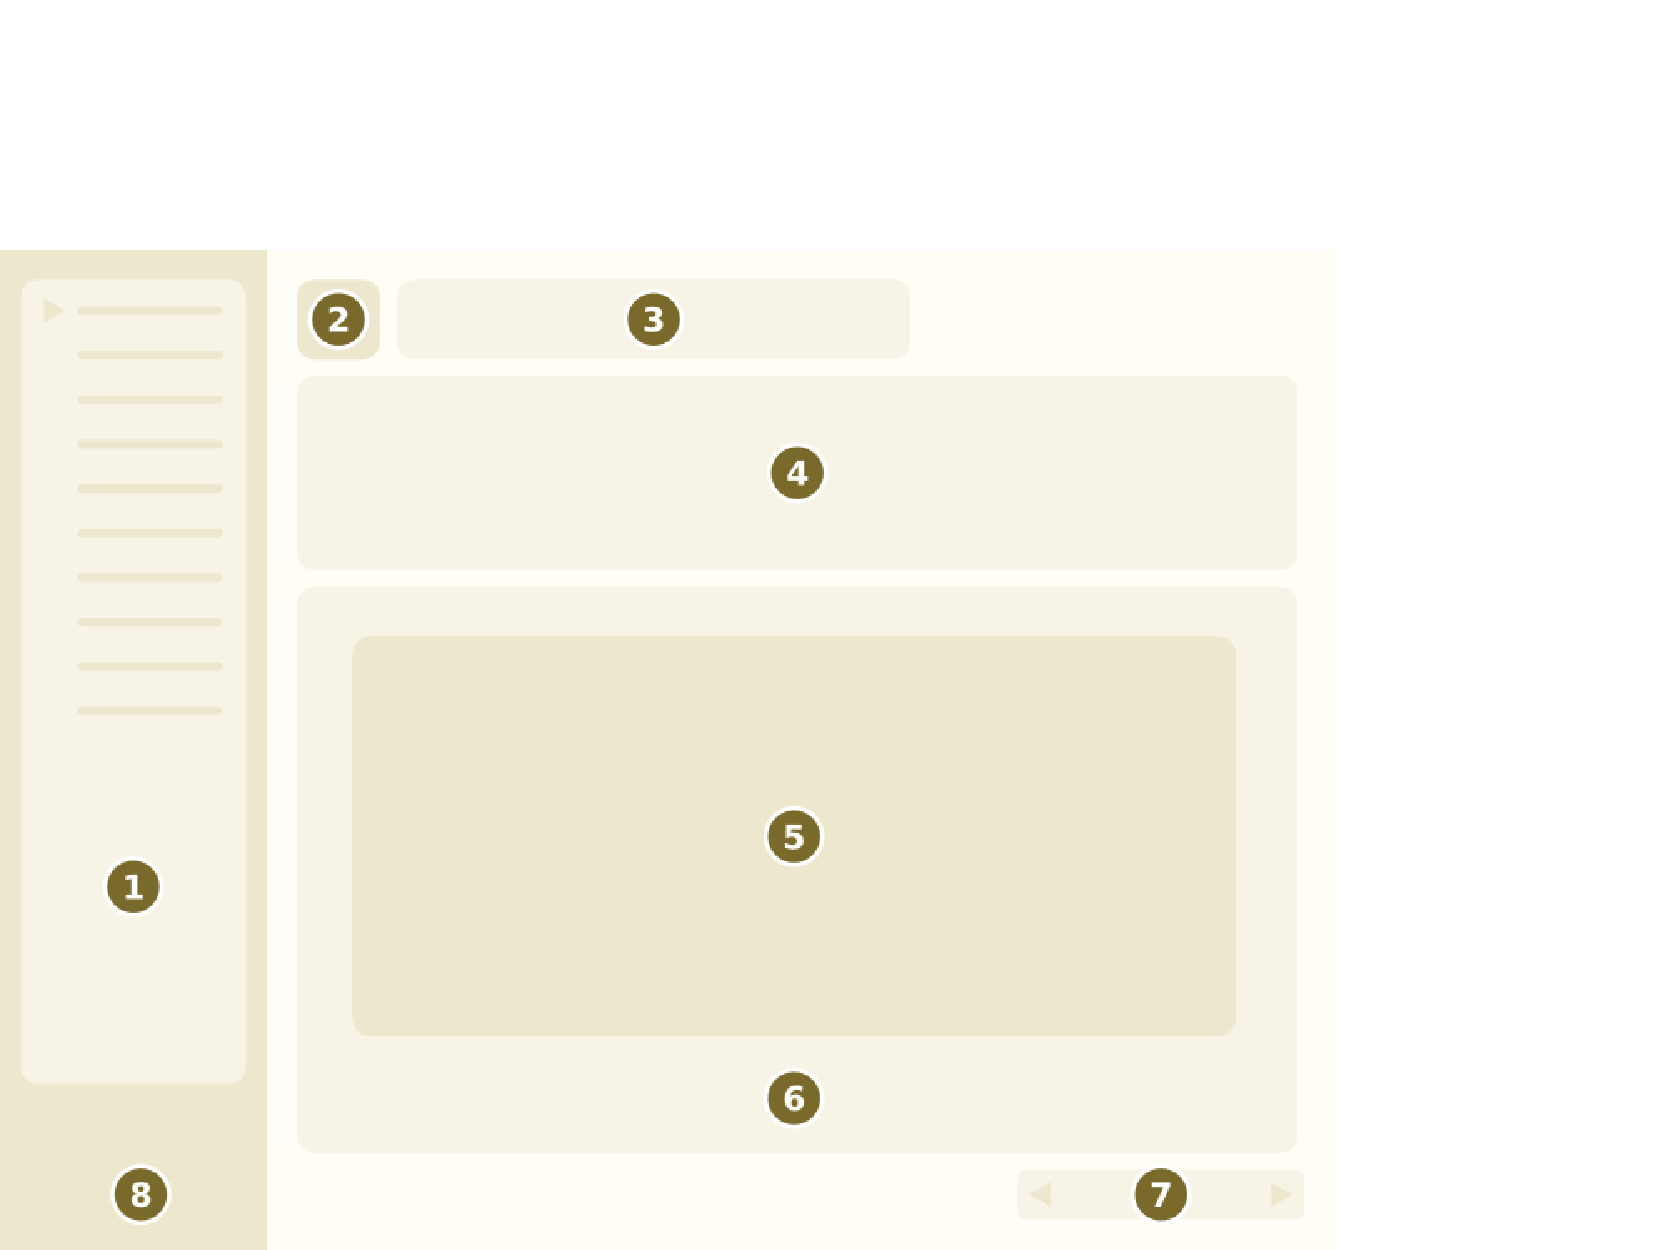
\includegraphics[width=0.8\textwidth]{%
../Identity/Models/Img/en/Distro/Anaconda/Firstboot/splash-small.pdf}}
\end{center}
\caption{Firstboot design model.%
   \label{fig:Distribution:Anaconda:Firstboot:Identity:Models}}
\end{figure}

\begin{description}

\item[1:] List of labels and a pointer showing in which configuration
screen you are.

\item[2:] Screen icon. The screen icon is visible in all firstboot
screens. Each firsboot screen may have its own screen icon.

\item[3:] Screen label.

\item[4:] Screen description. 

\item[5:] Splash image (splash-small.png). The splash
image is visible in firstboot welcome screen only.

\item[6:] Configuration stuff.

\item[7:] Navigation area. Basically two buttons to navegate
configuration back and forward.

\item[8:] List of labels' background image (firtboot-left.png).  This
image is visible in all firstboot screens.

\end{description}

\subsection{Image Files}
\hypertarget{sec:Distribution:Anaconda:Firstboot:Identity:Images}{}
\label{sec:Distribution:Anaconda:Firstboot:Identity:Images}

\begin{description}
\item[framework:]
trunk/Identity/Themes/\$THEME/Distro/Anaconda/Firstboot/Img/
\end{description}

\noindent Here is where firstboot final images are stored. 

\subsection{Image Files Rendering}
\hypertarget{sec:Distribution:Anaconda:Firstboot:Identity:ImagesRendering}{}
\label{sec:Distribution:Anaconda:Firstboot:Identity:ImagesRendering}

\begin{description}
\item[framework:]
trunk/Identity/Themes/\$THEME/Distro/Anaconda/Firstboot/
\end{description}

\noindent Here is where you produce firstboot images. The following
rendering examples, based on
\autoref{fig:Distribution:Anaconda:Firstboot:Translations}, illustrate
the firstboot image files rendering process.\\
\\
\fbox{\texttt{./render.sh}}\\
\\
\fbox{\texttt{./render.sh '(5|6)/splash'}}\\
\\
\fbox{\texttt{./render.sh '(firstboot-left|5|4)/splash'}}

\section{Translations}
\hypertarget{sec:Distribution:Anaconda:Firstboot:Translations}{}
\label{sec:Distribution:Anaconda:Firstboot:Translations}

\begin{description}
\item[framework:]
trunk/Translations/Identity/Themes/Distro/Anaconda/Firstboot
\end{description}

\noindent Here is where translators locale firstboot images. Image
localization is defined inside .sed files, also known as translation
files.  Translation files can be common or specific. The given
organization of translation files defines the translation path.

\begin{figure}[!hbp]
\hrulefill
\begin{verbatim}
trunk/Translations/Identity/Themes/Distro/Anaconda/Firstboot
|-- 3
|   `-- splash-small.sed
|-- 4
|   `-- splash-small.sed
|-- 5
|   `-- splash-small.sed
|-- ... (more release directories)
`-- firstboot-left.sed
\end{verbatim}
\hrulefill
\caption{Firstboot translation path.%
   \label{fig:Distribution:Anaconda:Firstboot:Translations}}
\end{figure}

\subsection{Translation Markers}

In firstboot, markers are used in the file splash-small.svg only,
specifically to set the major release number of CentOS Distribution in
CentOS Release Brand. Since firstboot-left.svg design is common for
all CentOS Distribution there is no need to set any marker on it.

Markers used in firstboot design templates and translation files are
described in \autoref{tab:Distribution:Anaconda:Firstboot:Markers}.

\begin{table}
\centering
\begin{tabular}{rl}
\hline
\textbf{Marker} & \textbf{Description}\\
\hline
=MAJOR\_RELEASE= & Major release number of CentOS Distribution.\\
\hline
\end{tabular}
\caption{Firstboot translation markers.%
   \label{tab:Distribution:Anaconda:Firstboot:Markers}}
\end{table}

\section{Manuals}
\hypertarget{sec:Distribution:Anaconda:Firstboot:Manuals}{}
\label{sec:Distribution:Anaconda:Firstboot:Manuals}

\begin{description}
\item[framework:]
trunk/Manuals/Distribution/Anaconda/Firstboot/
\end{description}

\noindent Here is where firstboot documentation is stored.  If you
want to help improving Firstboot documentation this is the place you
need to go.

\section{Scripts}
\hypertarget{sec:Distribution:Anaconda:Firstboot:Scripts}{}

\begin{description}
\item[framework:] trunk/Scripts/Config/Identity/Themes/Distro/Anaconda/Firstboot/
\end{description}

\noindent Here is stored the Firstboot \texttt{render.conf.sh}
configuration script.  To render Firstboot images correctly, the
\texttt{ARTCOMP} configuration variable inside Anaconda progress
configuration script should be defined as illustrated in
\autoref{fig:Distribution:Anaconda:Firstboot:Scripts:Config}. 

\begin{figure}
\hrulefill
\begin{verbatim}
# Define artwork component.
ARTCOMP='Identity/Themes/Distro/Anaconda/Firstboot'
\end{verbatim}
\hrulefill
\caption{Firstboot configuration layout.%
   \label{fig:Distribution:Anaconda:Firstboot:Scripts:Config}}
\end{figure}


   % Part   : Concepts
% Chapter: Rebranding
% ------------------------------------------------------------
% $Id: rebranding.tex 6191 2010-08-02 02:36:14Z al $
% ------------------------------------------------------------

To comply with upstream redistribution policy, the CentOS Project
removes all upstream brands and artworks from CentOS Distribution. The
CentOS Project has its own brand and its own artwork. The CentOS Brand
and CentOS Artwork are what the CentOS Project uses in CentOS
Distribution. 

The action of removing upstream brands and artworks and add CentOS
brands and artworks is what we call rebranding.

CentOS Brands and artworks are organized inside CentOS Artwork
Repository.  The CentOS Artwork Repository is maintain by CentOS
Artwork SIG which is formed by CentOS Community People.

\section{General Suggestions}

\begin{itemize}

\item Use original names as much as possible. Do not rename original
file names if you don't need to.

\end{itemize}



\chapter{Firstboot}
   \hypertarget{cha:Distribution:Anaconda:Firstboot}{}
   \label{cha:Distribution:Anaconda:Firstboot}
   %    Part: Distribution
% Chapter: Anaconda Progress - Introduction
% ------------------------------------------------------------
% $Id: introduction.tex 6019 2010-06-26 06:42:08Z al $
% ------------------------------------------------------------

Anaconda progress takes place after configuration screens and while
packages are being installed.  Anaconda progress visual style is
controlled by ``\hyperlink{cha:Distribution:Anaconda:Header}{Anaconda
Header}'' (\autoref{cha:Distribution:Anaconda:Header}), Anaconda
progress first slide, and Anaconda progress language-specific slides
set of images. Anaconda progress language-specific slides set of
images start rotating a few seconds after Anaconda progress first
slide.  It is possible for the user to alternate between Anaconda
progress slides and CentOS distribution
``\hyperlink{cha:Distribution:ReleaseNotes}{Release Notes}''
(\autoref{cha:Distribution:ReleaseNotes}).


   \section{Identity}
\hypertarget{sec:Distribution:Anaconda:Firstboot:Identity}{}
\label{sec:Distribution:Anaconda:Firstboot:Identity}

\begin{description}
\item[framework:]
trunk/Identity/Themes/\$THEME/Distro/Anaconda/Firstboot/
\end{description}

\noindent Here is where CentOS firstboot design templates and image
rendering take place. Firstboot identity file structure is illustrated
in \autoref{fig:Distribution:Anaconda:Firstboot:Identity} and
described in the following sections.

\begin{figure}
\hrulefill
\begin{verbatim}
trunk/Identity/Themes/$THEME/Distro/Anaconda/Firstboot/
|-- img
|   |-- 3
|   |   `-- splash-small.png
|   |-- 4
|   |   `-- splash-small.png
|   |-- 5
|   |   `-- splash-small.png
|   |-- ... (more releases here)
|   `-- firstboot-left.png
|-- render.sh
`-- tpl
    |-- firstboot-left.svg
        `-- splash-small.svg
\end{verbatim}
\hrulefill
\caption{Firstboot identity framework.%
   \label{fig:Distribution:Anaconda:Firstboot:Identity}}
\end{figure}

\subsection{Design Templates}

\begin{description}
\item[framework:]
trunk/Identity/Themes/\$THEME/Distro/Anaconda/Firstboot/Tpl/
\end{description}

\noindent Here is where Firstboot design templates are stored.
Firstboot design templates control Firstboot's visual style. 

\begin{description}

\item[firstboot-left.svg:] This design is common for all major
releases of CentOS Distribution. It is visible in all firstboot
screens. In
\autoref{fig:Distribution:Anaconda:Firstboot:Identity:Models}, this
design is illustraded by the number 8.

\item[splash-small.svg:] This design is specific for each major
release of CentOS Distribution.  There is one splash-small.png image
for each major release of CentOS Distribution. This image is visible
only in the first (Welcome) screen of Firstboot. In
\autoref{fig:Distribution:Anaconda:Firstboot:Identity:Models}, this
design is illustraded by number 5.

\end{description}

\subsection{Design Models}

\begin{description}
\item[framework:]
trunk/Identity/Models/Distro/Anaconda/Firstboot/
\end{description}

\noindent Here is where firstboot design models are stored. Firstboot
design model is shown in
\autoref{fig:Distribution:Anaconda:Firstboot:Identity:Models} and described
below: 

\begin{figure}
\begin{center}
\fbox{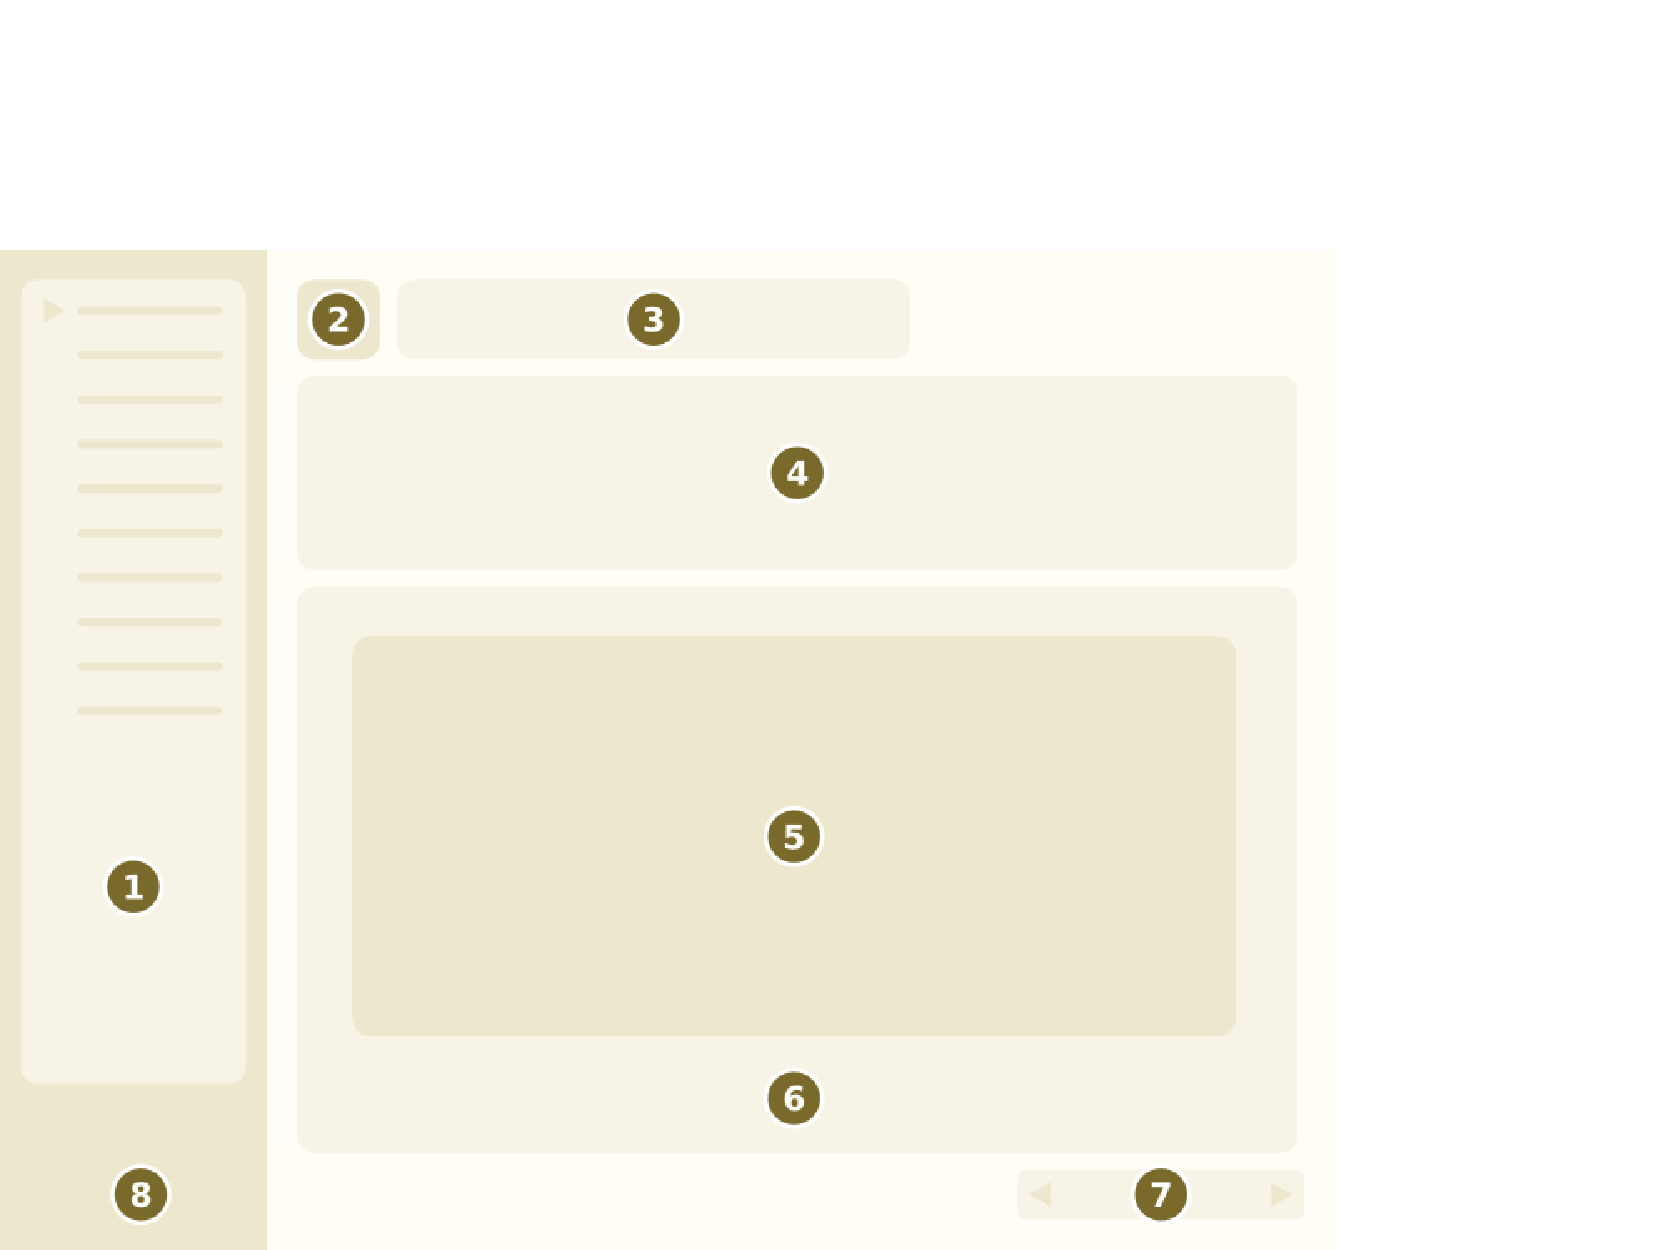
\includegraphics[width=0.8\textwidth]{%
../Identity/Models/Img/en/Distro/Anaconda/Firstboot/splash-small.pdf}}
\end{center}
\caption{Firstboot design model.%
   \label{fig:Distribution:Anaconda:Firstboot:Identity:Models}}
\end{figure}

\begin{description}

\item[1:] List of labels and a pointer showing in which configuration
screen you are.

\item[2:] Screen icon. The screen icon is visible in all firstboot
screens. Each firsboot screen may have its own screen icon.

\item[3:] Screen label.

\item[4:] Screen description. 

\item[5:] Splash image (splash-small.png). The splash
image is visible in firstboot welcome screen only.

\item[6:] Configuration stuff.

\item[7:] Navigation area. Basically two buttons to navegate
configuration back and forward.

\item[8:] List of labels' background image (firtboot-left.png).  This
image is visible in all firstboot screens.

\end{description}

\subsection{Image Files}
\hypertarget{sec:Distribution:Anaconda:Firstboot:Identity:Images}{}
\label{sec:Distribution:Anaconda:Firstboot:Identity:Images}

\begin{description}
\item[framework:]
trunk/Identity/Themes/\$THEME/Distro/Anaconda/Firstboot/Img/
\end{description}

\noindent Here is where firstboot final images are stored. 

\subsection{Image Files Rendering}
\hypertarget{sec:Distribution:Anaconda:Firstboot:Identity:ImagesRendering}{}
\label{sec:Distribution:Anaconda:Firstboot:Identity:ImagesRendering}

\begin{description}
\item[framework:]
trunk/Identity/Themes/\$THEME/Distro/Anaconda/Firstboot/
\end{description}

\noindent Here is where you produce firstboot images. The following
rendering examples, based on
\autoref{fig:Distribution:Anaconda:Firstboot:Translations}, illustrate
the firstboot image files rendering process.\\
\\
\fbox{\texttt{./render.sh}}\\
\\
\fbox{\texttt{./render.sh '(5|6)/splash'}}\\
\\
\fbox{\texttt{./render.sh '(firstboot-left|5|4)/splash'}}

\section{Translations}
\hypertarget{sec:Distribution:Anaconda:Firstboot:Translations}{}
\label{sec:Distribution:Anaconda:Firstboot:Translations}

\begin{description}
\item[framework:]
trunk/Translations/Identity/Themes/Distro/Anaconda/Firstboot
\end{description}

\noindent Here is where translators locale firstboot images. Image
localization is defined inside .sed files, also known as translation
files.  Translation files can be common or specific. The given
organization of translation files defines the translation path.

\begin{figure}[!hbp]
\hrulefill
\begin{verbatim}
trunk/Translations/Identity/Themes/Distro/Anaconda/Firstboot
|-- 3
|   `-- splash-small.sed
|-- 4
|   `-- splash-small.sed
|-- 5
|   `-- splash-small.sed
|-- ... (more release directories)
`-- firstboot-left.sed
\end{verbatim}
\hrulefill
\caption{Firstboot translation path.%
   \label{fig:Distribution:Anaconda:Firstboot:Translations}}
\end{figure}

\subsection{Translation Markers}

In firstboot, markers are used in the file splash-small.svg only,
specifically to set the major release number of CentOS Distribution in
CentOS Release Brand. Since firstboot-left.svg design is common for
all CentOS Distribution there is no need to set any marker on it.

Markers used in firstboot design templates and translation files are
described in \autoref{tab:Distribution:Anaconda:Firstboot:Markers}.

\begin{table}
\centering
\begin{tabular}{rl}
\hline
\textbf{Marker} & \textbf{Description}\\
\hline
=MAJOR\_RELEASE= & Major release number of CentOS Distribution.\\
\hline
\end{tabular}
\caption{Firstboot translation markers.%
   \label{tab:Distribution:Anaconda:Firstboot:Markers}}
\end{table}

\section{Manuals}
\hypertarget{sec:Distribution:Anaconda:Firstboot:Manuals}{}
\label{sec:Distribution:Anaconda:Firstboot:Manuals}

\begin{description}
\item[framework:]
trunk/Manuals/Distribution/Anaconda/Firstboot/
\end{description}

\noindent Here is where firstboot documentation is stored.  If you
want to help improving Firstboot documentation this is the place you
need to go.

\section{Scripts}
\hypertarget{sec:Distribution:Anaconda:Firstboot:Scripts}{}

\begin{description}
\item[framework:] trunk/Scripts/Config/Identity/Themes/Distro/Anaconda/Firstboot/
\end{description}

\noindent Here is stored the Firstboot \texttt{render.conf.sh}
configuration script.  To render Firstboot images correctly, the
\texttt{ARTCOMP} configuration variable inside Anaconda progress
configuration script should be defined as illustrated in
\autoref{fig:Distribution:Anaconda:Firstboot:Scripts:Config}. 

\begin{figure}
\hrulefill
\begin{verbatim}
# Define artwork component.
ARTCOMP='Identity/Themes/Distro/Anaconda/Firstboot'
\end{verbatim}
\hrulefill
\caption{Firstboot configuration layout.%
   \label{fig:Distribution:Anaconda:Firstboot:Scripts:Config}}
\end{figure}


   % Part   : Concepts
% Chapter: Rebranding
% ------------------------------------------------------------
% $Id: rebranding.tex 6191 2010-08-02 02:36:14Z al $
% ------------------------------------------------------------

To comply with upstream redistribution policy, the CentOS Project
removes all upstream brands and artworks from CentOS Distribution. The
CentOS Project has its own brand and its own artwork. The CentOS Brand
and CentOS Artwork are what the CentOS Project uses in CentOS
Distribution. 

The action of removing upstream brands and artworks and add CentOS
brands and artworks is what we call rebranding.

CentOS Brands and artworks are organized inside CentOS Artwork
Repository.  The CentOS Artwork Repository is maintain by CentOS
Artwork SIG which is formed by CentOS Community People.

\section{General Suggestions}

\begin{itemize}

\item Use original names as much as possible. Do not rename original
file names if you don't need to.

\end{itemize}



\chapter{GNOME Display Manager (GDM)}
   \hypertarget{cha:Distribution:BootUp:GDM}{}
   \label{cha:Distribution:BootUp:GDM}

\chapter{GRand Unified Bootloader (GRUB)}
   \hypertarget{cha:Distribution:BootUp:GRUB}{}
   \label{cha:Distribution:BootUp:GRUB}

\chapter{GNOME Splash}
   \hypertarget{cha:Distribution:BootUp:GSplash}{}
   \label{cha:Distribution:BootUp:GSplash}

\chapter{KDE Display Manager (KDM)}
   \hypertarget{cha:Distribution:BootUp:KDM}{}
   \label{cha:Distribution:BootUp:KDM}

\chapter{KDE Splash}
   \hypertarget{cha:Distribution:BootUp:KSplash}{}
   \label{cha:Distribution:BootUp:KSplash}

\chapter{Graphical Boot (RHGB)}
   \hypertarget{cha:Distribution:BootUp:RHGB}{}
   \label{cha:Distribution:BootUp:RHGB}

\chapter{Backgrounds}
   \hypertarget{cha:Distribution:Backgrounds}{}
   \label{cha:Distribution:Backgrounds}
   %    Part: Distribution
% Chapter: Anaconda Progress - Introduction
% ------------------------------------------------------------
% $Id: introduction.tex 6019 2010-06-26 06:42:08Z al $
% ------------------------------------------------------------

Anaconda progress takes place after configuration screens and while
packages are being installed.  Anaconda progress visual style is
controlled by ``\hyperlink{cha:Distribution:Anaconda:Header}{Anaconda
Header}'' (\autoref{cha:Distribution:Anaconda:Header}), Anaconda
progress first slide, and Anaconda progress language-specific slides
set of images. Anaconda progress language-specific slides set of
images start rotating a few seconds after Anaconda progress first
slide.  It is possible for the user to alternate between Anaconda
progress slides and CentOS distribution
``\hyperlink{cha:Distribution:ReleaseNotes}{Release Notes}''
(\autoref{cha:Distribution:ReleaseNotes}).


   \section{Identity}
\hypertarget{sec:Distribution:Anaconda:Firstboot:Identity}{}
\label{sec:Distribution:Anaconda:Firstboot:Identity}

\begin{description}
\item[framework:]
trunk/Identity/Themes/\$THEME/Distro/Anaconda/Firstboot/
\end{description}

\noindent Here is where CentOS firstboot design templates and image
rendering take place. Firstboot identity file structure is illustrated
in \autoref{fig:Distribution:Anaconda:Firstboot:Identity} and
described in the following sections.

\begin{figure}
\hrulefill
\begin{verbatim}
trunk/Identity/Themes/$THEME/Distro/Anaconda/Firstboot/
|-- img
|   |-- 3
|   |   `-- splash-small.png
|   |-- 4
|   |   `-- splash-small.png
|   |-- 5
|   |   `-- splash-small.png
|   |-- ... (more releases here)
|   `-- firstboot-left.png
|-- render.sh
`-- tpl
    |-- firstboot-left.svg
        `-- splash-small.svg
\end{verbatim}
\hrulefill
\caption{Firstboot identity framework.%
   \label{fig:Distribution:Anaconda:Firstboot:Identity}}
\end{figure}

\subsection{Design Templates}

\begin{description}
\item[framework:]
trunk/Identity/Themes/\$THEME/Distro/Anaconda/Firstboot/Tpl/
\end{description}

\noindent Here is where Firstboot design templates are stored.
Firstboot design templates control Firstboot's visual style. 

\begin{description}

\item[firstboot-left.svg:] This design is common for all major
releases of CentOS Distribution. It is visible in all firstboot
screens. In
\autoref{fig:Distribution:Anaconda:Firstboot:Identity:Models}, this
design is illustraded by the number 8.

\item[splash-small.svg:] This design is specific for each major
release of CentOS Distribution.  There is one splash-small.png image
for each major release of CentOS Distribution. This image is visible
only in the first (Welcome) screen of Firstboot. In
\autoref{fig:Distribution:Anaconda:Firstboot:Identity:Models}, this
design is illustraded by number 5.

\end{description}

\subsection{Design Models}

\begin{description}
\item[framework:]
trunk/Identity/Models/Distro/Anaconda/Firstboot/
\end{description}

\noindent Here is where firstboot design models are stored. Firstboot
design model is shown in
\autoref{fig:Distribution:Anaconda:Firstboot:Identity:Models} and described
below: 

\begin{figure}
\begin{center}
\fbox{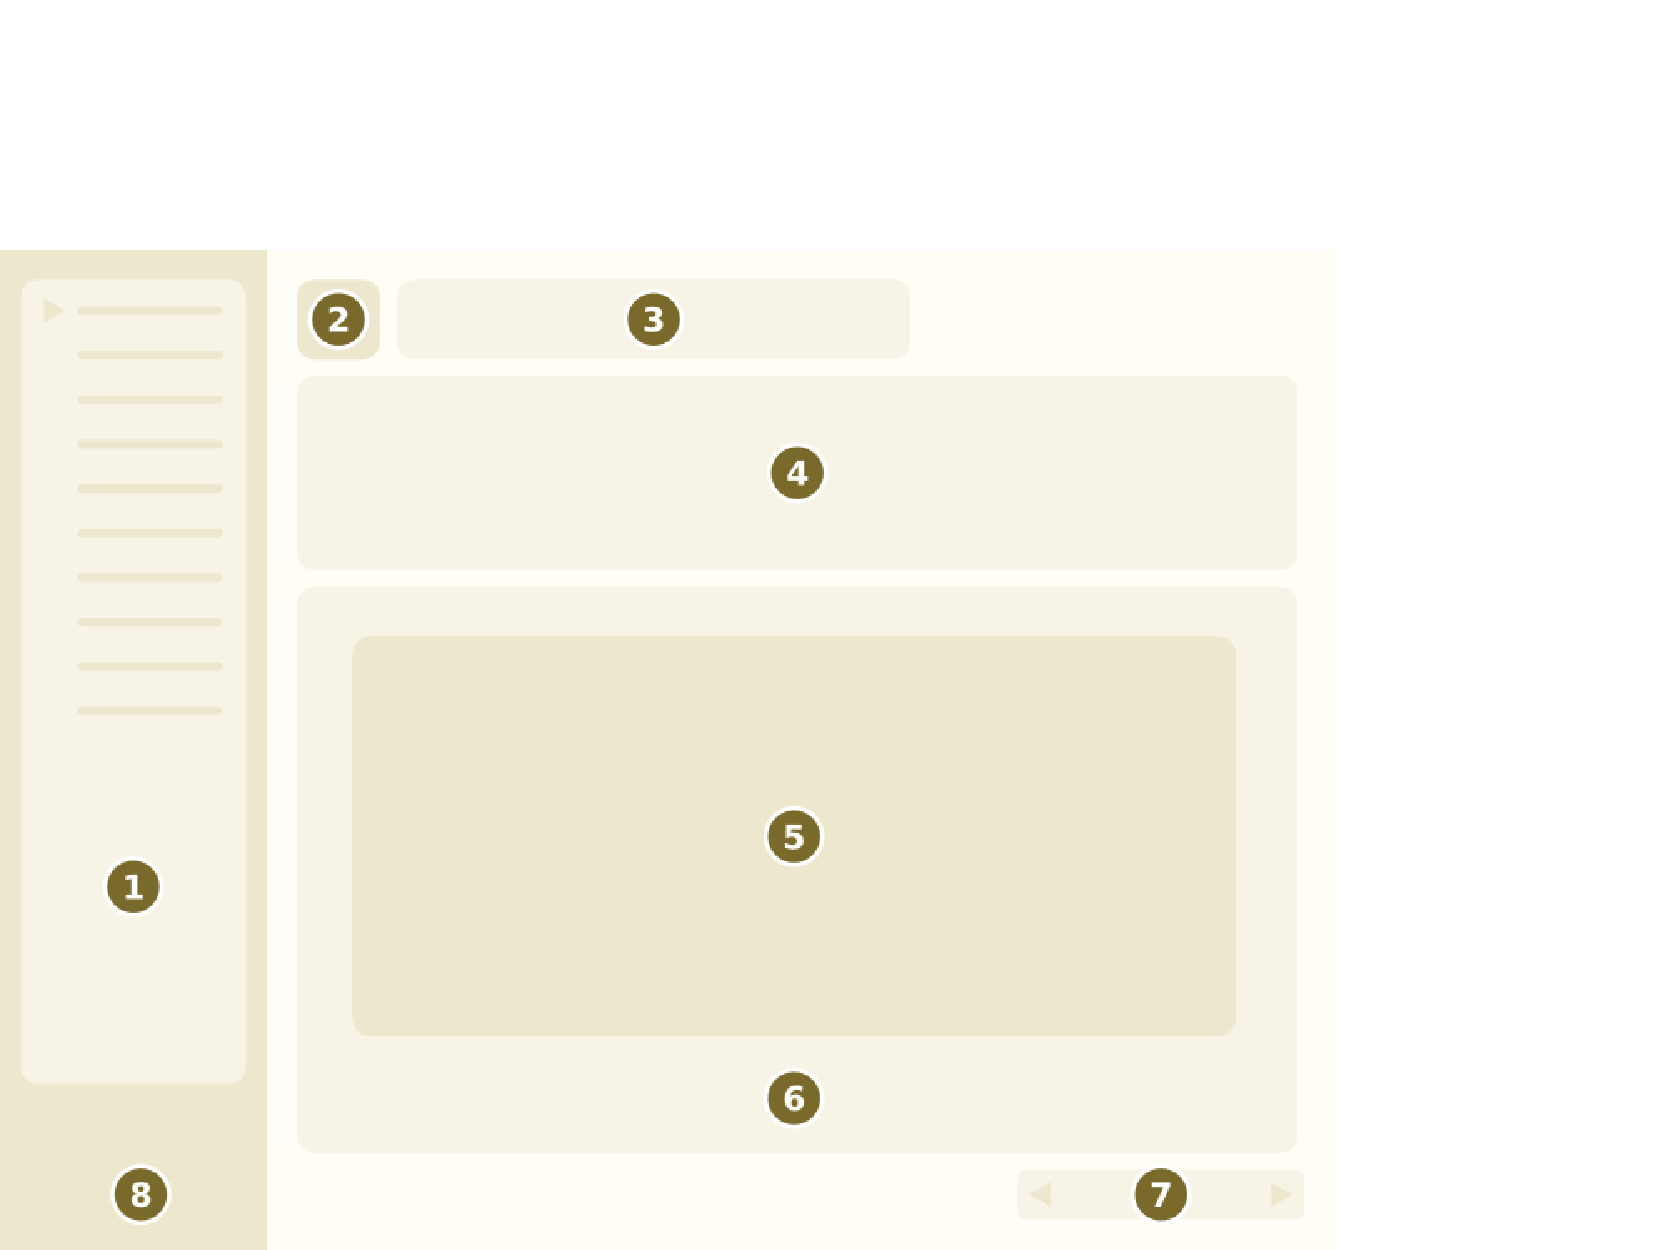
\includegraphics[width=0.8\textwidth]{%
../Identity/Models/Img/en/Distro/Anaconda/Firstboot/splash-small.pdf}}
\end{center}
\caption{Firstboot design model.%
   \label{fig:Distribution:Anaconda:Firstboot:Identity:Models}}
\end{figure}

\begin{description}

\item[1:] List of labels and a pointer showing in which configuration
screen you are.

\item[2:] Screen icon. The screen icon is visible in all firstboot
screens. Each firsboot screen may have its own screen icon.

\item[3:] Screen label.

\item[4:] Screen description. 

\item[5:] Splash image (splash-small.png). The splash
image is visible in firstboot welcome screen only.

\item[6:] Configuration stuff.

\item[7:] Navigation area. Basically two buttons to navegate
configuration back and forward.

\item[8:] List of labels' background image (firtboot-left.png).  This
image is visible in all firstboot screens.

\end{description}

\subsection{Image Files}
\hypertarget{sec:Distribution:Anaconda:Firstboot:Identity:Images}{}
\label{sec:Distribution:Anaconda:Firstboot:Identity:Images}

\begin{description}
\item[framework:]
trunk/Identity/Themes/\$THEME/Distro/Anaconda/Firstboot/Img/
\end{description}

\noindent Here is where firstboot final images are stored. 

\subsection{Image Files Rendering}
\hypertarget{sec:Distribution:Anaconda:Firstboot:Identity:ImagesRendering}{}
\label{sec:Distribution:Anaconda:Firstboot:Identity:ImagesRendering}

\begin{description}
\item[framework:]
trunk/Identity/Themes/\$THEME/Distro/Anaconda/Firstboot/
\end{description}

\noindent Here is where you produce firstboot images. The following
rendering examples, based on
\autoref{fig:Distribution:Anaconda:Firstboot:Translations}, illustrate
the firstboot image files rendering process.\\
\\
\fbox{\texttt{./render.sh}}\\
\\
\fbox{\texttt{./render.sh '(5|6)/splash'}}\\
\\
\fbox{\texttt{./render.sh '(firstboot-left|5|4)/splash'}}

\section{Translations}
\hypertarget{sec:Distribution:Anaconda:Firstboot:Translations}{}
\label{sec:Distribution:Anaconda:Firstboot:Translations}

\begin{description}
\item[framework:]
trunk/Translations/Identity/Themes/Distro/Anaconda/Firstboot
\end{description}

\noindent Here is where translators locale firstboot images. Image
localization is defined inside .sed files, also known as translation
files.  Translation files can be common or specific. The given
organization of translation files defines the translation path.

\begin{figure}[!hbp]
\hrulefill
\begin{verbatim}
trunk/Translations/Identity/Themes/Distro/Anaconda/Firstboot
|-- 3
|   `-- splash-small.sed
|-- 4
|   `-- splash-small.sed
|-- 5
|   `-- splash-small.sed
|-- ... (more release directories)
`-- firstboot-left.sed
\end{verbatim}
\hrulefill
\caption{Firstboot translation path.%
   \label{fig:Distribution:Anaconda:Firstboot:Translations}}
\end{figure}

\subsection{Translation Markers}

In firstboot, markers are used in the file splash-small.svg only,
specifically to set the major release number of CentOS Distribution in
CentOS Release Brand. Since firstboot-left.svg design is common for
all CentOS Distribution there is no need to set any marker on it.

Markers used in firstboot design templates and translation files are
described in \autoref{tab:Distribution:Anaconda:Firstboot:Markers}.

\begin{table}
\centering
\begin{tabular}{rl}
\hline
\textbf{Marker} & \textbf{Description}\\
\hline
=MAJOR\_RELEASE= & Major release number of CentOS Distribution.\\
\hline
\end{tabular}
\caption{Firstboot translation markers.%
   \label{tab:Distribution:Anaconda:Firstboot:Markers}}
\end{table}

\section{Manuals}
\hypertarget{sec:Distribution:Anaconda:Firstboot:Manuals}{}
\label{sec:Distribution:Anaconda:Firstboot:Manuals}

\begin{description}
\item[framework:]
trunk/Manuals/Distribution/Anaconda/Firstboot/
\end{description}

\noindent Here is where firstboot documentation is stored.  If you
want to help improving Firstboot documentation this is the place you
need to go.

\section{Scripts}
\hypertarget{sec:Distribution:Anaconda:Firstboot:Scripts}{}

\begin{description}
\item[framework:] trunk/Scripts/Config/Identity/Themes/Distro/Anaconda/Firstboot/
\end{description}

\noindent Here is stored the Firstboot \texttt{render.conf.sh}
configuration script.  To render Firstboot images correctly, the
\texttt{ARTCOMP} configuration variable inside Anaconda progress
configuration script should be defined as illustrated in
\autoref{fig:Distribution:Anaconda:Firstboot:Scripts:Config}. 

\begin{figure}
\hrulefill
\begin{verbatim}
# Define artwork component.
ARTCOMP='Identity/Themes/Distro/Anaconda/Firstboot'
\end{verbatim}
\hrulefill
\caption{Firstboot configuration layout.%
   \label{fig:Distribution:Anaconda:Firstboot:Scripts:Config}}
\end{figure}


   % Part   : Concepts
% Chapter: Rebranding
% ------------------------------------------------------------
% $Id: rebranding.tex 6191 2010-08-02 02:36:14Z al $
% ------------------------------------------------------------

To comply with upstream redistribution policy, the CentOS Project
removes all upstream brands and artworks from CentOS Distribution. The
CentOS Project has its own brand and its own artwork. The CentOS Brand
and CentOS Artwork are what the CentOS Project uses in CentOS
Distribution. 

The action of removing upstream brands and artworks and add CentOS
brands and artworks is what we call rebranding.

CentOS Brands and artworks are organized inside CentOS Artwork
Repository.  The CentOS Artwork Repository is maintain by CentOS
Artwork SIG which is formed by CentOS Community People.

\section{General Suggestions}

\begin{itemize}

\item Use original names as much as possible. Do not rename original
file names if you don't need to.

\end{itemize}



\chapter{Release Notes}
   \hypertarget{cha:Distribution:ReleaseNotes}{}
   \label{cha:Distribution:ReleaseNotes}

\part{Promotion}

\chapter{Cards}
   \hypertarget{cha:Promotion:Cards}{}
   \label{cha:Promotion:Cards}

\chapter{Clothes}
   \hypertarget{cha:Promotion:Clothes}{}
   \label{cha:Promotion:Clothes}

\chapter{Flags}
   \hypertarget{cha:Promotion:Flags}{}
   \label{cha:Promotion:Flags}

\chapter{Media}
   \hypertarget{cha:Promotion:Media}{}
   \label{cha:Promotion:Media}

\chapter{Posters}
   \hypertarget{cha:Promotion:Posters}{}
   \label{cha:Promotion:Posters}
   
\chapter{Releases}
   \hypertarget{cha:Promotion:Releases}{}
   \label{cha:Promotion:Releases}

\chapter{Stands}
   \hypertarget{cha:Promotion:Stands}{}
   \label{cha:Promotion:Stands}

\chapter{Stationery}
   \hypertarget{cha:Promotion:Stationery}{}
   \label{cha:Promotion:Stationery}

\chapter{Sticky}
   \hypertarget{cha:Promotion:Sticky}{}
   \label{cha:Promotion:Sticky}

\part{Licenses}
\appendix
%
% CentOS Redistribution License.
%
\chapter{CentOS Redistribution License}
\noindent Revision 1.0, March 2010\\
\noindent Copyright \copyright\ 2010 The CentOS Project.\\
\\
\noindent The \texttt{redhat-logos} and \texttt{redhat-artwork}
packages (the ``Packages'') contain image files which incorporate the
CentOS trademark, and CentOS logo (the ``Marks'').

The CentOS Project grants you the right to use the Packages during the
normal operation of other software programs that call upon the
Packages.  The CentOS Project grants to you the right and license to
copy and redistribute the unaltered Packages for both commerical and
non-commercial purposes.

If you are rebranding or modifying the underlying distribution, or the
Packages, you must remove ``the Marks'' and rename the distribution
something other than CentOS.

When redistributing using this license, the following applies:

\begin{enumerate}

\item The above copyright notice and this license are included with
each copy you make, and they remain intact and are not altered,
deleted, or modified in any way;

\item You do not modify the appearance of any or all of the Logos in
any manner; and

\item You do not use any or all of the Logos as, or as part of, a
trademark, trade name, or trade identifier; or in any other fashion
except as set forth in this license.

\item No Warranty. The Packages are provided ``as are'' and any
express or implied warranties, including, but not limited to, the
implied warranties of merchantability and fitness for a particular
purpose are disclaimed. In no event shall the CentOS Project be liable
for any direct, indirect, incidental, special, exemplary, or
consequential damages ---including, but not limited to, procurement of
substitute goods or services; loss of use, data or profits; or
business interruption--- however caused and on any theory of
liability, whether in contract, strict liability, or tort ---including
negligence or otherwise--- arising in any way out of the use of this
package, even if advised of the possibility of such damage.

\end{enumerate}



% Verbatim copy of GNU Free Documentation License. The License under
% which this document is released.
\chapter{GNU Free Documentation License}
\hypertarget{cha:Licenses:GFDL}{}
\label{cha:Licenses:GFDL}

Version 1.2, November 2002
\\
\\
Copyright \copyright\ 2000,2001,2002 Free Software Foundation, Inc.  
\\
59 Temple Place, Suite 330, Boston, MA  02111-1307, USA
\\
Everyone is permitted to copy and distribute verbatim copies of this
license document, but changing it is not allowed.

\section*{Preamble}
\label{sec:License-GFDL-0}

The purpose of this License is to make a manual, textbook, or other
functional and useful document ``free'' in the sense of freedom: to
assure everyone the effective freedom to copy and redistribute it,
with or without modifying it, either commercially or noncommercially.
Secondarily, this License preserves for the author and publisher a way
to get credit for their work, while not being considered responsible
for modifications made by others.

This License is a kind of ``copyleft'', which means that derivative
works of the document must themselves be free in the same sense.  It
complements the GNU General Public License, which is a copyleft
license designed for free software.

We have designed this License in order to use it for manuals for free
software, because free software needs free documentation: a free
program should come with manuals providing the same freedoms that the
software does.  But this License is not limited to software manuals;
it can be used for any textual work, regardless of subject matter or
whether it is published as a printed book.  We recommend this License
principally for works whose purpose is instruction or reference.

\section{Applicability And Definitions}
\label{sec:License-GFDL-1}

This License applies to any manual or other work, in any medium, that
contains a notice placed by the copyright holder saying it can be
distributed under the terms of this License.  Such a notice grants a
world-wide, royalty-free license, unlimited in duration, to use that
work under the conditions stated herein.  The ``Document'', below,
refers to any such manual or work.  Any member of the public is a
licensee, and is addressed as ``you''.  You accept the license if you
copy, modify or distribute the work in a way requiring permission
under copyright law.

A ``Modified Version'' of the Document means any work containing the
Document or a portion of it, either copied verbatim, or with
modifications and/or translated into another language.

A ``Secondary Section'' is a named appendix or a front-matter section of
the Document that deals exclusively with the relationship of the
publishers or authors of the Document to the Document's overall
subject (or to related matters) and contains nothing that could fall
directly within that overall subject.  (Thus, if the Document is in
part a textbook of mathematics, a Secondary Section may not explain
any mathematics.)  The relationship could be a matter of historical
connection with the subject or with related matters, or of legal,
commercial, philosophical, ethical or political position regarding
them.

The ``Invariant Sections'' are certain Secondary Sections whose titles
are designated, as being those of Invariant Sections, in the notice
that says that the Document is released under this License.  If a
section does not fit the above definition of Secondary then it is not
allowed to be designated as Invariant.  The Document may contain zero
Invariant Sections.  If the Document does not identify any Invariant
Sections then there are none.

The ``Cover Texts'' are certain short passages of text that are listed,
as Front-Cover Texts or Back-Cover Texts, in the notice that says that
the Document is released under this License.  A Front-Cover Text may
be at most 5 words, and a Back-Cover Text may be at most 25 words.

A ``Transparent'' copy of the Document means a machine-readable copy,
represented in a format whose specification is available to the
general public, that is suitable for revising the document
straightforwardly with generic text editors or (for images composed of
pixels) generic paint programs or (for drawings) some widely available
drawing editor, and that is suitable for input to text formatters or
for automatic translation to a variety of formats suitable for input
to text formatters.  A copy made in an otherwise Transparent file
format whose markup, or absence of markup, has been arranged to thwart
or discourage subsequent modification by readers is not Transparent.
An image format is not Transparent if used for any substantial amount
of text.  A copy that is not ``Transparent'' is called ``Opaque''.

Examples of suitable formats for Transparent copies include plain
ASCII without markup, Texinfo input format, \LaTeX\ input format, SGML
or XML using a publicly available DTD, and standard-conforming simple
HTML, PostScript or PDF designed for human modification.  Examples of
transparent image formats include PNG, XCF and JPG.  Opaque formats
include proprietary formats that can be read and edited only by
proprietary word processors, SGML or XML for which the DTD and/or
processing tools are not generally available, and the
machine-generated HTML, PostScript or PDF produced by some word
processors for output purposes only.

The ``Title Page'' means, for a printed book, the title page itself,
plus such following pages as are needed to hold, legibly, the material
this License requires to appear in the title page.  For works in
formats which do not have any title page as such, ``Title Page'' means
the text near the most prominent appearance of the work's title,
preceding the beginning of the body of the text.

A section ``Entitled XYZ'' means a named subunit of the Document whose
title either is precisely XYZ or contains XYZ in parentheses following
text that translates XYZ in another language.  (Here XYZ stands for a
specific section name mentioned below, such as ``Acknowledgements'',
``Dedications'', ``Endorsements'', or ``History''.) To ``Preserve the
Title'' of such a section when you modify the Document means that it
remains a section ``Entitled XYZ'' according to this definition.

The Document may include Warranty Disclaimers next to the notice which
states that this License applies to the Document.  These Warranty
Disclaimers are considered to be included by reference in this
License, but only as regards disclaiming warranties: any other
implication that these Warranty Disclaimers may have is void and has
no effect on the meaning of this License.

\section{Verbatim Copying}
\label{sec:License-GFDL-2}

You may copy and distribute the Document in any medium, either
commercially or noncommercially, provided that this License, the
copyright notices, and the license notice saying this License applies
to the Document are reproduced in all copies, and that you add no
other conditions whatsoever to those of this License.  You may not use
technical measures to obstruct or control the reading or further
copying of the copies you make or distribute.  However, you may accept
compensation in exchange for copies.  If you distribute a large enough
number of copies you must also follow the conditions in section
\ref{sec:License-GFDL-3}.

You may also lend copies, under the same conditions stated above, and
you may publicly display copies.

\section{Copying In Quantity}
\label{sec:License-GFDL-3}

If you publish printed copies (or copies in media that commonly have
printed covers) of the Document, numbering more than 100, and the
Document's license notice requires Cover Texts, you must enclose the
copies in covers that carry, clearly and legibly, all these Cover
Texts: Front-Cover Texts on the front cover, and Back-Cover Texts on
the back cover.  Both covers must also clearly and legibly identify
you as the publisher of these copies.  The front cover must present
the full title with all words of the title equally prominent and
visible.  You may add other material on the covers in addition.
Copying with changes limited to the covers, as long as they preserve
the title of the Document and satisfy these conditions, can be treated
as verbatim copying in other respects.

If the required texts for either cover are too voluminous to fit
legibly, you should put the first ones listed (as many as fit
reasonably) on the actual cover, and continue the rest onto adjacent
pages.

If you publish or distribute Opaque copies of the Document numbering
more than 100, you must either include a machine-readable Transparent
copy along with each Opaque copy, or state in or with each Opaque copy
a computer-network location from which the general network-using
public has access to download using public-standard network protocols
a complete Transparent copy of the Document, free of added material.
If you use the latter option, you must take reasonably prudent steps,
when you begin distribution of Opaque copies in quantity, to ensure
that this Transparent copy will remain thus accessible at the stated
location until at least one year after the last time you distribute an
Opaque copy (directly or through your agents or retailers) of that
edition to the public.

It is requested, but not required, that you contact the authors of the
Document well before redistributing any large number of copies, to
give them a chance to provide you with an updated version of the
Document.

\section{Modifications}
\label{sec:License-GFDL-4}

You may copy and distribute a Modified Version of the Document under
the conditions of sections \ref{sec:License-GFDL-2} and
\ref{sec:License-GFDL-3} above, provided that you release the Modified
Version under precisely this License, with the Modified Version
filling the role of the Document, thus licensing distribution and
modification of the Modified Version to whoever possesses a copy of
it.  In addition, you must do these things in the Modified Version:

\begin{itemize}

\item [A.] Use in the Title Page (and on the covers, if any) a title
distinct from that of the Document, and from those of previous
versions (which should, if there were any, be listed in the History
section of the Document).  You may use the same title as a previous
version if the original publisher of that version gives permission.

\item [B.] List on the Title Page, as authors, one or more persons or
entities responsible for authorship of the modifications in the
Modified Version, together with at least five of the principal authors
of the Document (all of its principal authors, if it has fewer than
five), unless they release you from this requirement.

\item [C.] State on the Title page the name of the publisher of the
Modified Version, as the publisher.

\item [D.] Preserve all the copyright notices of the Document.

\item [E.] Add an appropriate copyright notice for your modifications
adjacent to the other copyright notices.

\item [F.] Include, immediately after the copyright notices, a license
notice giving the public permission to use the Modified Version under
the terms of this License, in the form shown in the Addendum below.

\item [G.] Preserve in that license notice the full lists of Invariant
Sections and required Cover Texts given in the Document's license
notice.

\item [H.] Include an unaltered copy of this License.

\item [I.] Preserve the section Entitled ``History'', Preserve its
Title, and add to it an item stating at least the title, year, new
authors, and publisher of the Modified Version as given on the Title
Page.  If there is no section Entitled ``History'' in the Document,
create one stating the title, year, authors, and publisher of the
Document as given on its Title Page, then add an item describing the
Modified Version as stated in the previous sentence.

\item [J.] Preserve the network location, if any, given in the
Document for public access to a Transparent copy of the Document, and
likewise the network locations given in the Document for previous
versions it was based on.  These may be placed in the ``History''
section.  You may omit a network location for a work that was
published at least four years before the Document itself, or if the
original publisher of the version it refers to gives permission.

\item [K.] For any section Entitled ``Acknowledgements'' or
``Dedications'', Preserve the Title of the section, and preserve in
the section all the substance and tone of each of the contributor
acknowledgements and/or dedications given therein.

\item [L.] Preserve all the Invariant Sections of the Document,
unaltered in their text and in their titles.  Section numbers or the
equivalent are not considered part of the section titles.

\item [M.] Delete any section Entitled ``Endorsements''.  Such a
section may not be included in the Modified Version.

\item [N.] Do not retitle any existing section to be Entitled
``Endorsements'' or to conflict in title with any Invariant Section.

\item [O.] Preserve any Warranty Disclaimers.
\end{itemize}

If the Modified Version includes new front-matter sections or
appendices that qualify as Secondary Sections and contain no material
copied from the Document, you may at your option designate some or all
of these sections as invariant.  To do this, add their titles to the
list of Invariant Sections in the Modified Version's license notice.
These titles must be distinct from any other section titles.

You may add a section Entitled ``Endorsements'', provided it contains
nothing but endorsements of your Modified Version by various
parties--for example, statements of peer review or that the text has
been approved by an organization as the authoritative definition of a
standard.

You may add a passage of up to five words as a Front-Cover Text, and a
passage of up to 25 words as a Back-Cover Text, to the end of the list
of Cover Texts in the Modified Version.  Only one passage of
Front-Cover Text and one of Back-Cover Text may be added by (or
through arrangements made by) any one entity.  If the Document already
includes a cover text for the same cover, previously added by you or
by arrangement made by the same entity you are acting on behalf of,
you may not add another; but you may replace the old one, on explicit
permission from the previous publisher that added the old one.

The author(s) and publisher(s) of the Document do not by this License
give permission to use their names for publicity for or to assert or
imply endorsement of any Modified Version.

\section{Combining Documents}
\label{sec:License-GFDL-5}

You may combine the Document with other documents released under this
License, under the terms defined in section \ref{sec:License-GFDL-4}
above for modified versions, provided that you include in the
combination all of the Invariant Sections of all of the original
documents, unmodified, and list them all as Invariant Sections of your
combined work in its license notice, and that you preserve all their
Warranty Disclaimers.

The combined work need only contain one copy of this License, and
multiple identical Invariant Sections may be replaced with a single
copy.  If there are multiple Invariant Sections with the same name but
different contents, make the title of each such section unique by
adding at the end of it, in parentheses, the name of the original
author or publisher of that section if known, or else a unique number.
Make the same adjustment to the section titles in the list of
Invariant Sections in the license notice of the combined work.

In the combination, you must combine any sections Entitled ``History''
in the various original documents, forming one section Entitled
``History''; likewise combine any sections Entitled
``Acknowledgements'',
and any sections Entitled ``Dedications''.  You must delete all sections
Entitled ``Endorsements''.

\section{Collections Of Documents}
\label{sec:License-GFDL-6}

You may make a collection consisting of the Document and other
documents released under this License, and replace the individual
copies of this License in the various documents with a single copy
that is included in the collection, provided that you follow the rules
of this License for verbatim copying of each of the documents in all
other respects.

You may extract a single document from such a collection, and
distribute it individually under this License, provided you insert a
copy of this License into the extracted document, and follow this
License in all other respects regarding verbatim copying of that
document.

\section{Aggregation With Independent Works}
\label{sec:License-GFDL-7}

A compilation of the Document or its derivatives with other separate
and independent documents or works, in or on a volume of a storage or
distribution medium, is called an ``aggregate'' if the copyright
resulting from the compilation is not used to limit the legal rights
of the compilation's users beyond what the individual works permit.
When the Document is included in an aggregate, this License does not
apply to the other works in the aggregate which are not themselves
derivative works of the Document.

If the Cover Text requirement of section \ref{sec:License-GFDL-3} is
applicable to these copies of the Document, then if the Document is
less than one half of the entire aggregate, the Document's Cover Texts
may be placed on covers that bracket the Document within the
aggregate, or the electronic equivalent of covers if the Document is
in electronic form.  Otherwise they must appear on printed covers that
bracket the whole aggregate.

\section{Translation}
\label{sec:License-GFDL-8}

Translation is considered a kind of modification, so you may
distribute translations of the Document under the terms of section
\ref{sec:License-GFDL-4}.  Replacing Invariant Sections with
translations requires special permission from their copyright holders,
but you may include translations of some or all Invariant Sections in
addition to the original versions of these Invariant Sections.  You
may include a translation of this License, and all the license notices
in the Document, and any Warranty Disclaimers, provided that you also
include the original English version of this License and the original
versions of those notices and disclaimers.  In case of a disagreement
between the translation and the original version of this License or a
notice or disclaimer, the original version will prevail.

If a section in the Document is Entitled ``Acknowledgements'',
``Dedications'', or ``History'', the requirement (section
\ref{sec:License-GFDL-4}) to Preserve its Title (section
\ref{sec:License-GFDL-1}) will typically require changing the actual
title.

\section{Termination}
\label{sec:License-GFDL-9}

You may not copy, modify, sublicense, or distribute the Document
except as expressly provided for under this License.  Any other
attempt to copy, modify, sublicense or distribute the Document is
void, and will automatically terminate your rights under this License.
However, parties who have received copies, or rights, from you under
this License will not have their licenses terminated so long as such
parties remain in full compliance.

\section{Future Revisions Of This License}
\label{sec:License-GFDL-10}

The Free Software Foundation may publish new, revised versions of the
GNU Free Documentation License from time to time.  Such new versions
will be similar in spirit to the present version, but may differ in
detail to address new problems or concerns.  See
\url{http://www.gnu.org/copyleft/}.

Each version of the License is given a distinguishing version number.
If the Document specifies that a particular numbered version of this
License ``or any later version'' applies to it, you have the option of
following the terms and conditions either of that specified version or
of any later version that has been published (not as a draft) by the
Free Software Foundation.  If the Document does not specify a version
number of this License, you may choose any version ever published (not
as a draft) by the Free Software Foundation.

\section{How to use this License for your documents}
\label{sec:License-GFDL-11}

To use this License in a document you have written, include a copy of
the License in the document and put the following copyright and
license notices just after the title page:

\begin{verbatim}
   Copyright (C)  YEAR  YOUR NAME.

   Permission is granted to copy, distribute and/or modify this
   document under the terms of the GNU Free Documentation License,
   Version 1.2 or any later version published by the Free Software
   Foundation; with no Invariant Sections, no Front-Cover Texts,
   and no Back-Cover Texts.  A copy of the license is included in
   the section entitled ``GNU Free Documentation License''.
\end{verbatim}

If you have Invariant Sections, Front-Cover Texts and Back-Cover
Texts, replace the ``with...Texts''. line with this:

\begin{verbatim}
   with the Invariant Sections being LIST THEIR TITLES, with the
   Front-Cover Texts being LIST, and with the Back-Cover Texts
   being LIST.
\end{verbatim}

If you have Invariant Sections without Cover Texts, or some other
combination of the three, merge those two alternatives to suit the
situation.

If your document contains nontrivial examples of program code, we
recommend releasing these examples in parallel under your choice of
free software license, such as the GNU General Public License, to
permit their use in free software.



\backmatter

% Bibliographies: BibTeX automates much of the job of typesetting
% bibliographies, and makes bibliography entries reusable in many
% different contexts.

% Indexing table: 

\end{document}
